% EFFECTIVE HAMILTONIAN FOR PWE
\section*{Effective Hamiltonian for uMPS plane wave excitations}
In the actual \textit{matvec} implementation of $H_{\mathrm{eff}}(p)$ \eqref{eq:Heff_p}, we compute $B = V_L X$, then $\Tilde{\tket{B}} = H_{\mathrm{eff}}(p) \tket{B}$, and in the end we transform back to $\Tilde{X} = \overline{V_L} \Tilde{B}$. In the following we draw all tensor diagrams appearing in the expectation value
\begin{equation*}
	\textcolor{blue}{\tbra{\overline{B}}} H_{\mathrm{eff}}(p) \textcolor{blue}{\tket{B}} = \sum_{m, n \in \mathbb{Z}} e^{ipm} \raisebox{-0.5\height}{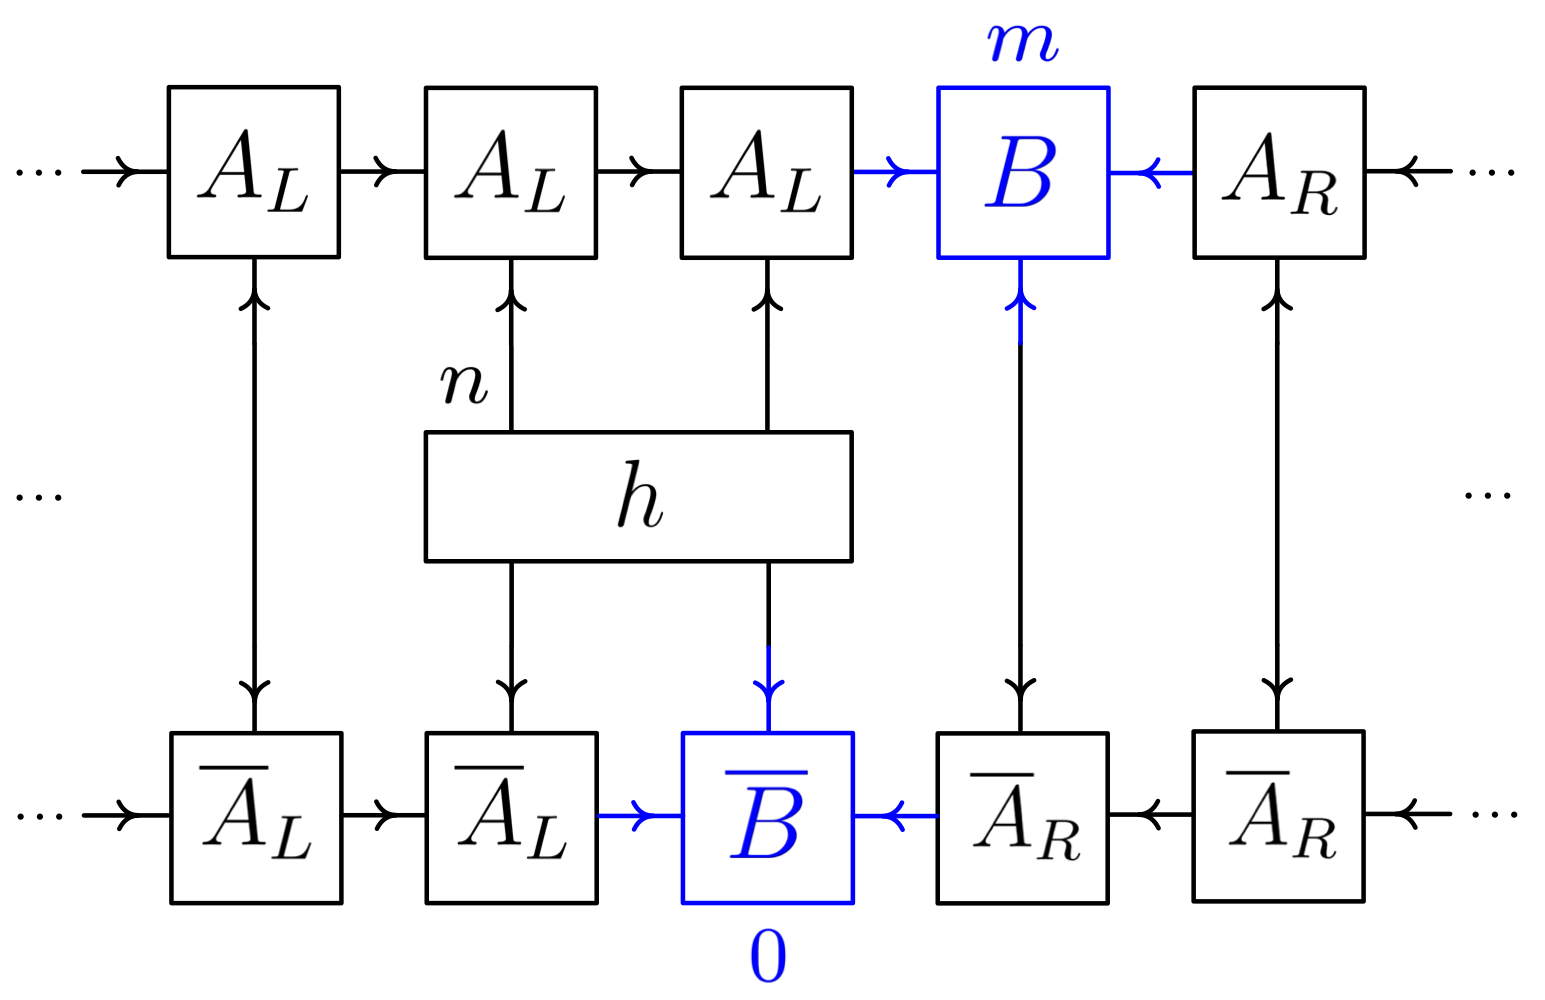
\includegraphics[height=4.5cm]{B_H_B.png}} \hspace{0.2em} .
\end{equation*}

\begin{center}

1) $m = -1, \ldots, - \infty$ 

\vspace{1em} 

1a) $n = -2, \ldots, - \infty$ 
\begin{equation*}
	e^{-ip} 
	\raisebox{-0.5\height}{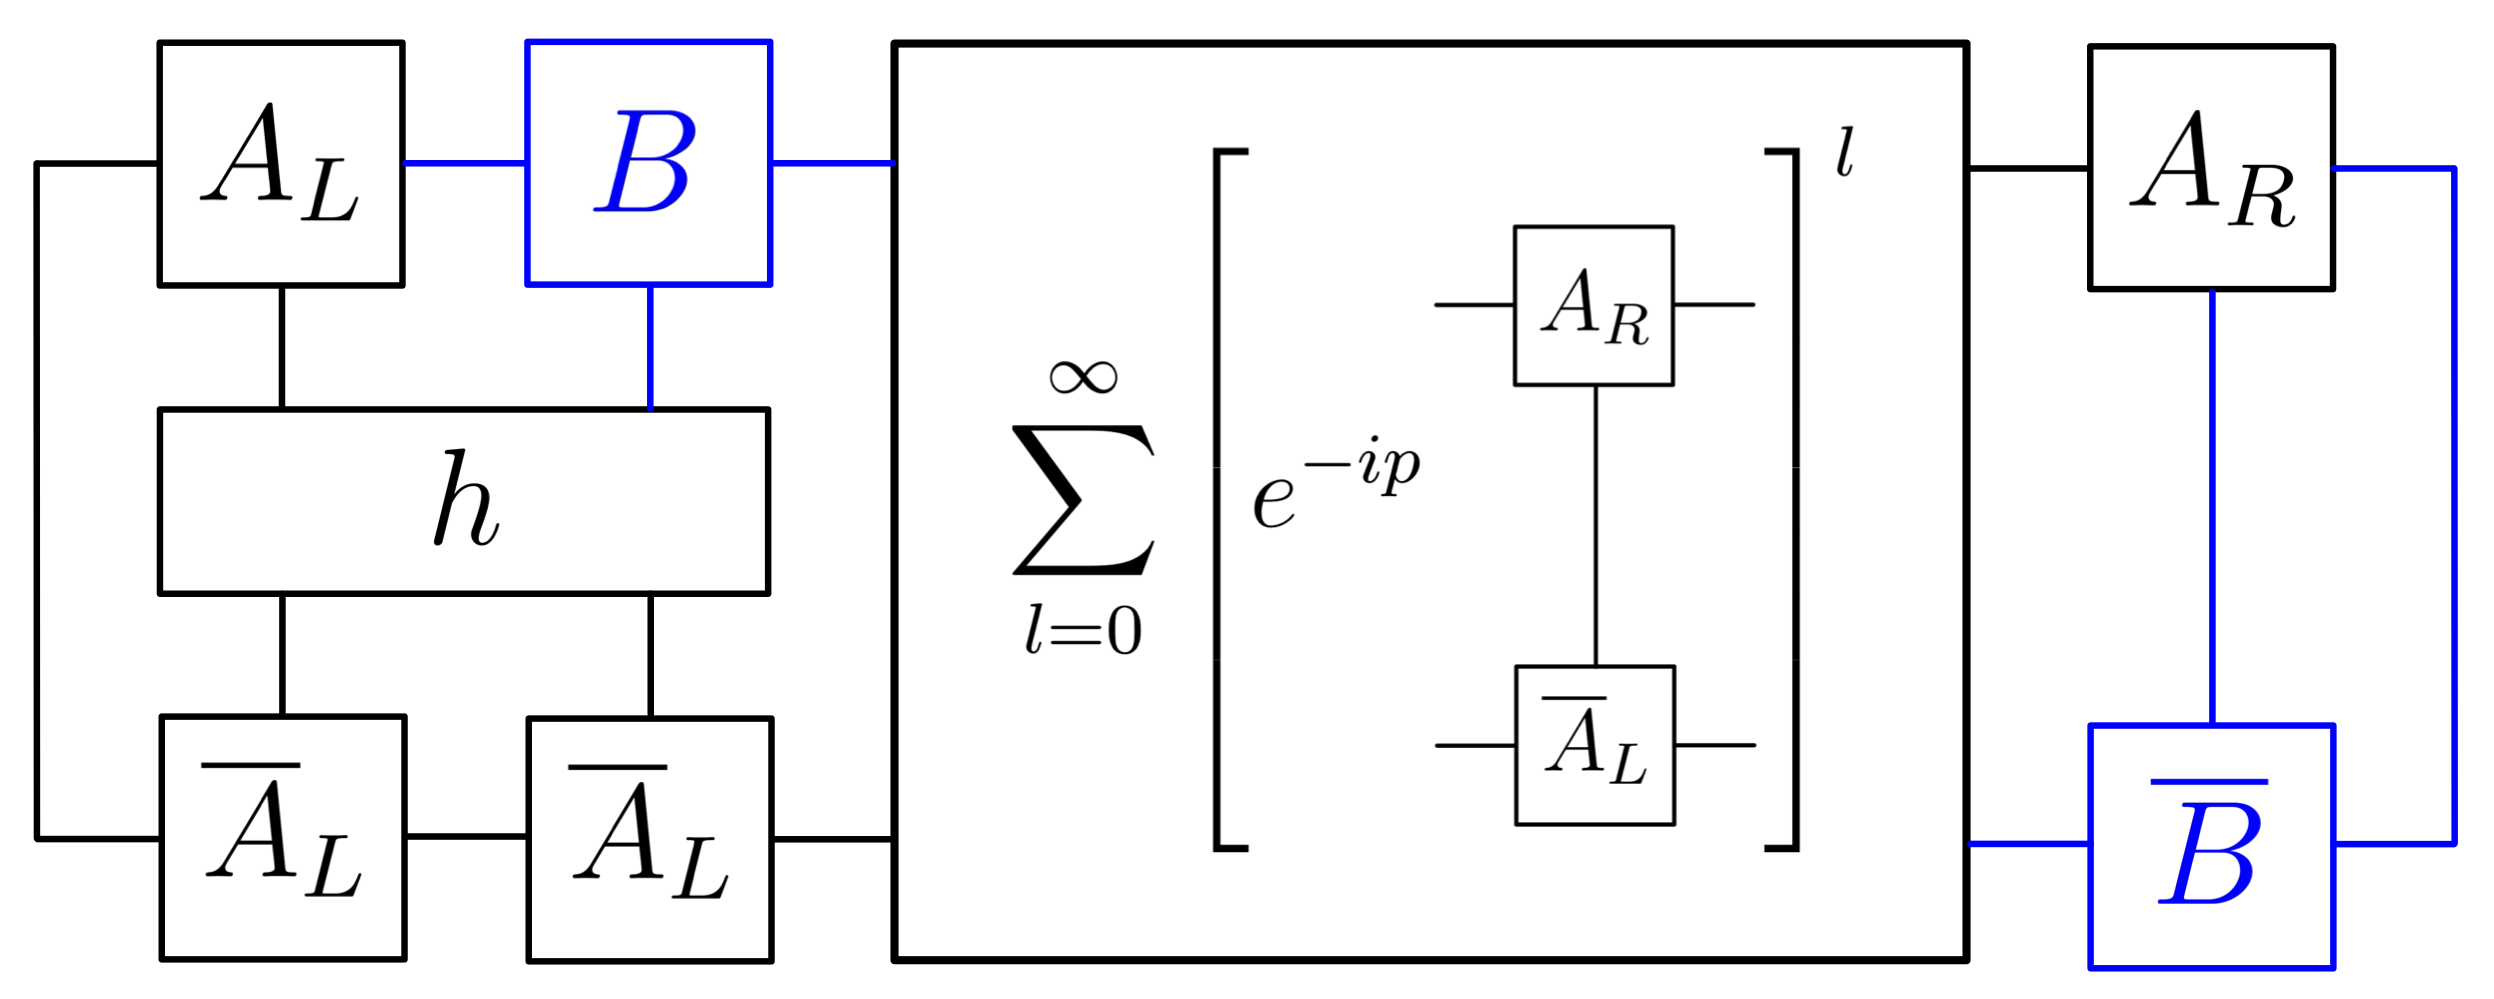
\includegraphics[height=3cm]{b1.png}} 
	\: + \: 
	e^{-2ip} 
	\raisebox{-0.5\height}{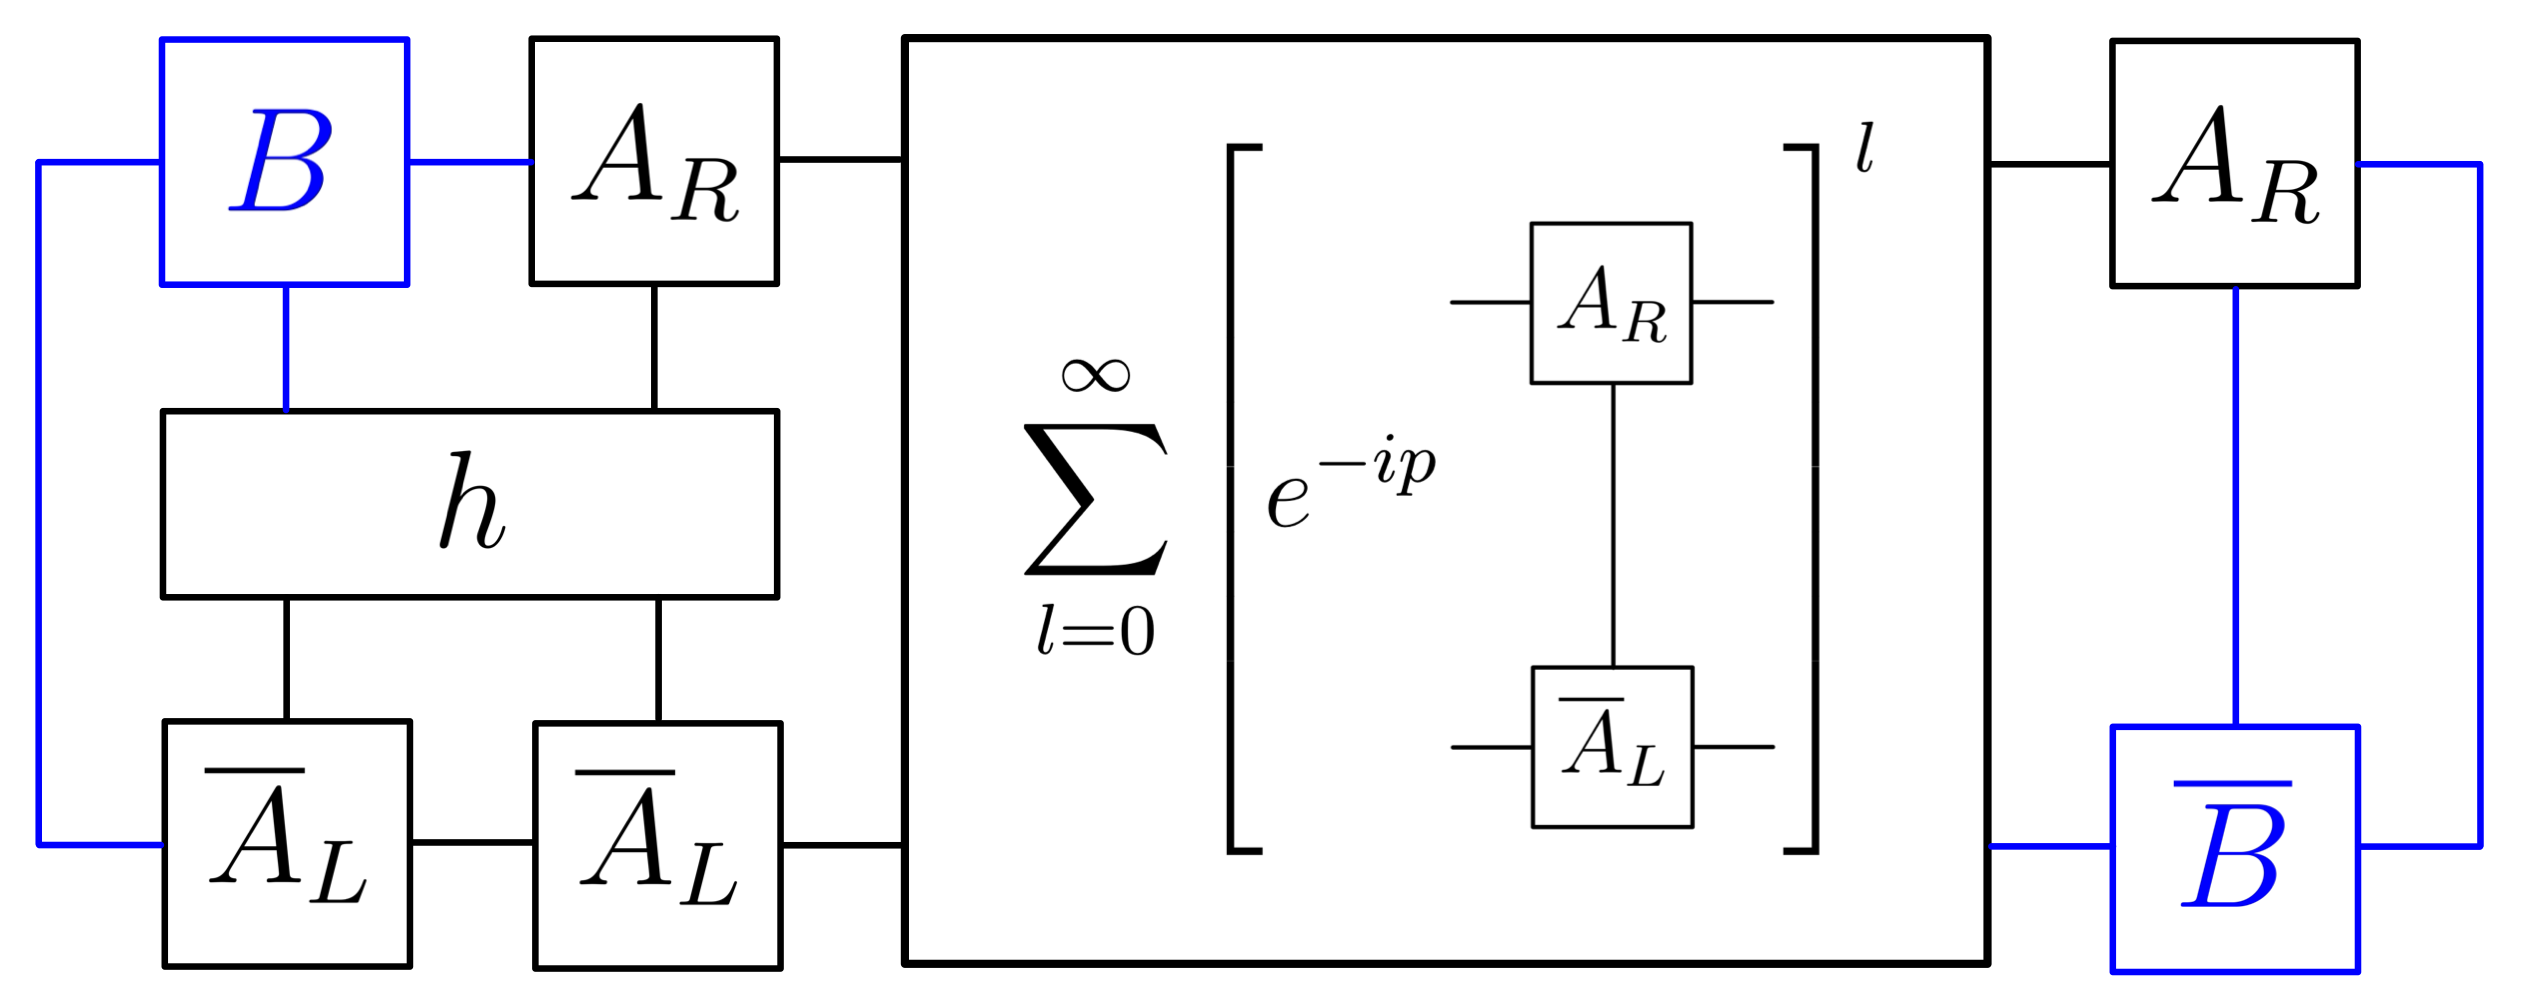
\includegraphics[height=3cm]{b2.png}} 
\end{equation*}
\begin{equation*}
	\: + \: 
	\underbrace{e^{-3ip} 
	\raisebox{-0.5\height}{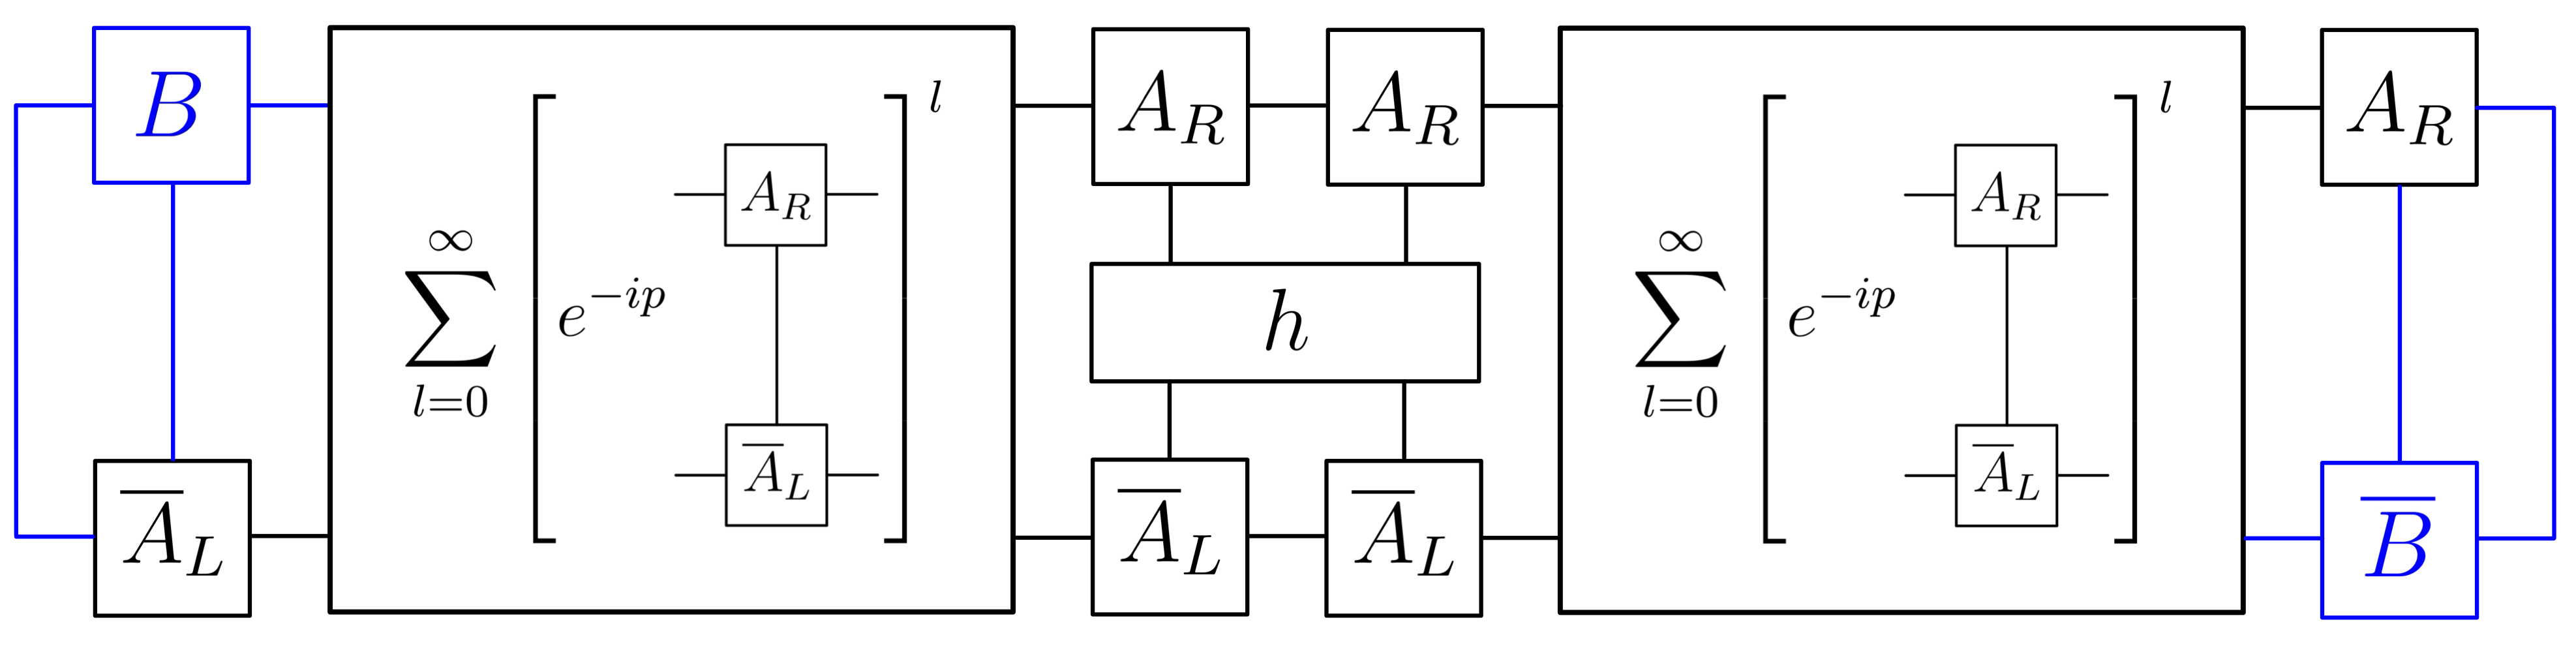
\includegraphics[height=3cm]{b3.png}}}_{=0} 
\end{equation*}
\begin{equation*}
	\: + \: e^{-ip} 
	\raisebox{-0.5\height}{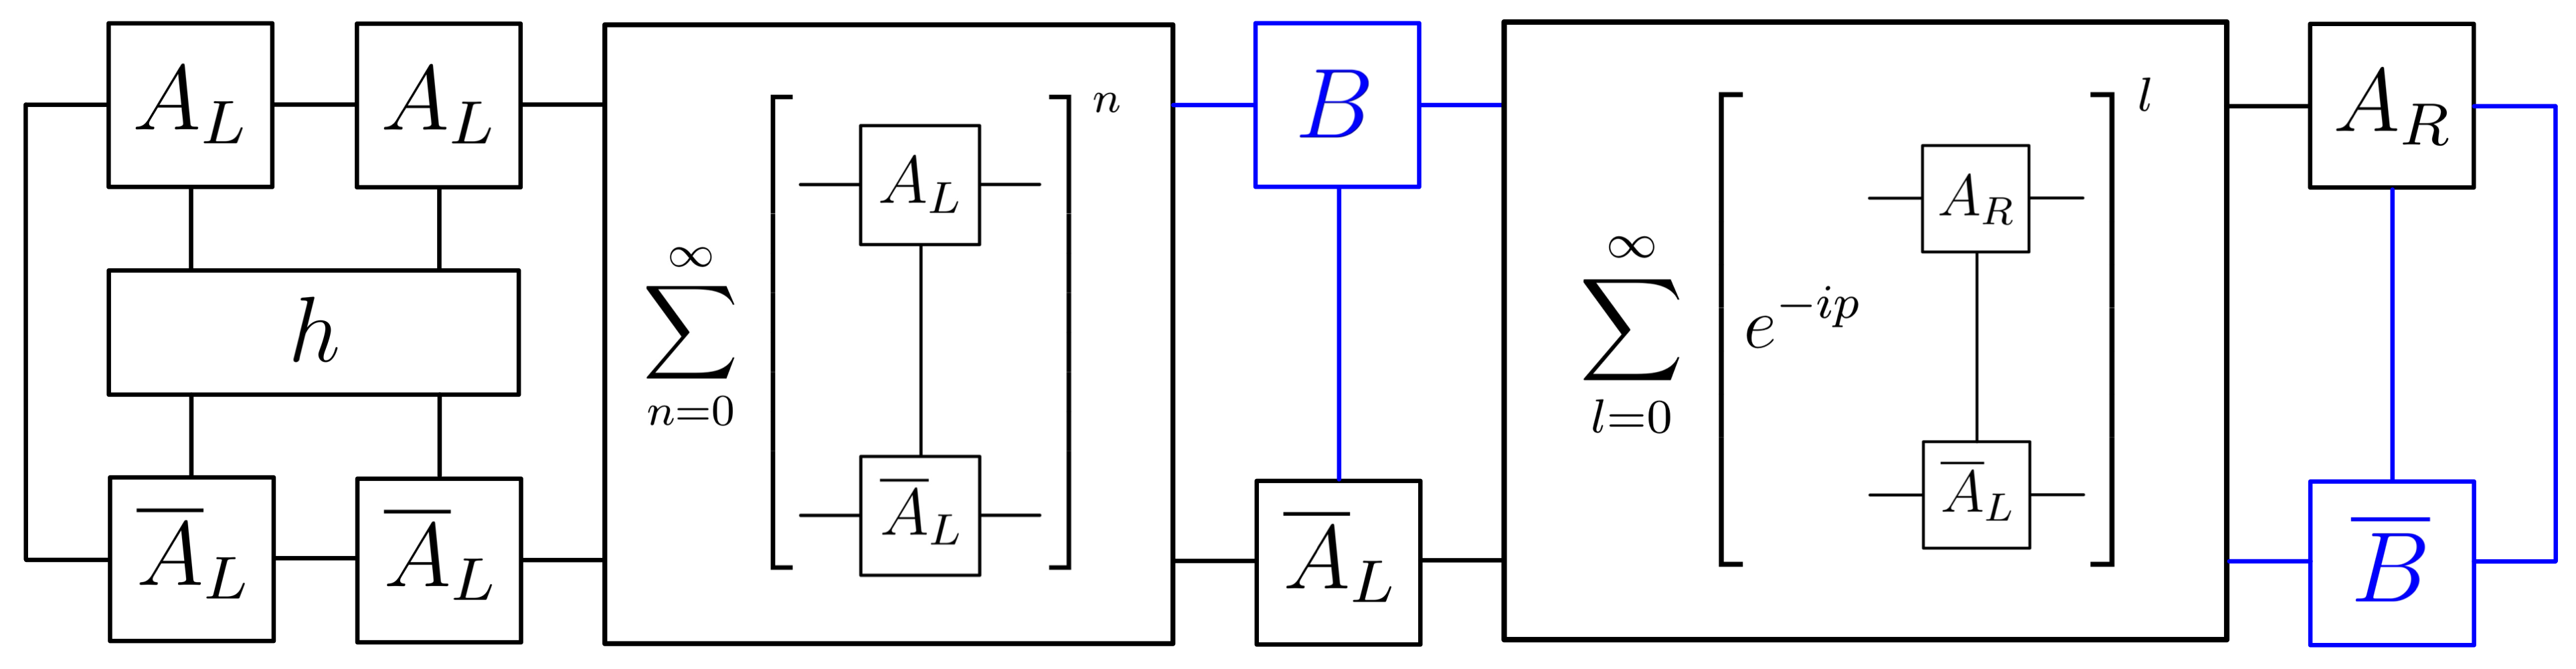
\includegraphics[height=3cm]{b4.png}} 
\end{equation*}

\vspace{1em} 

1b) $n = -1$ 
\begin{equation*}
	\: + \: e^{-ip} 
	\raisebox{-0.5\height}{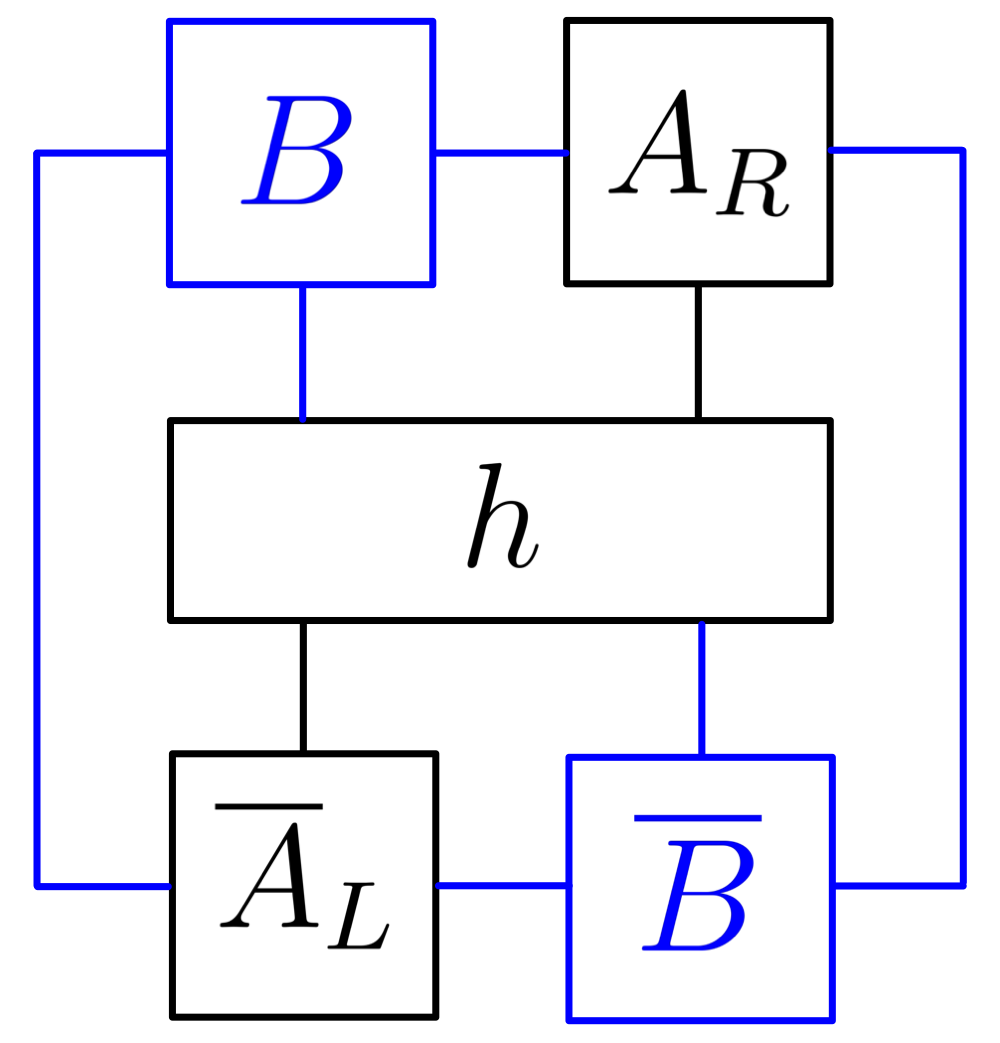
\includegraphics[height=3cm]{b5.png}} 
	\: + \: 
	\underbrace{e^{-2ip} 
	\raisebox{-0.5\height}{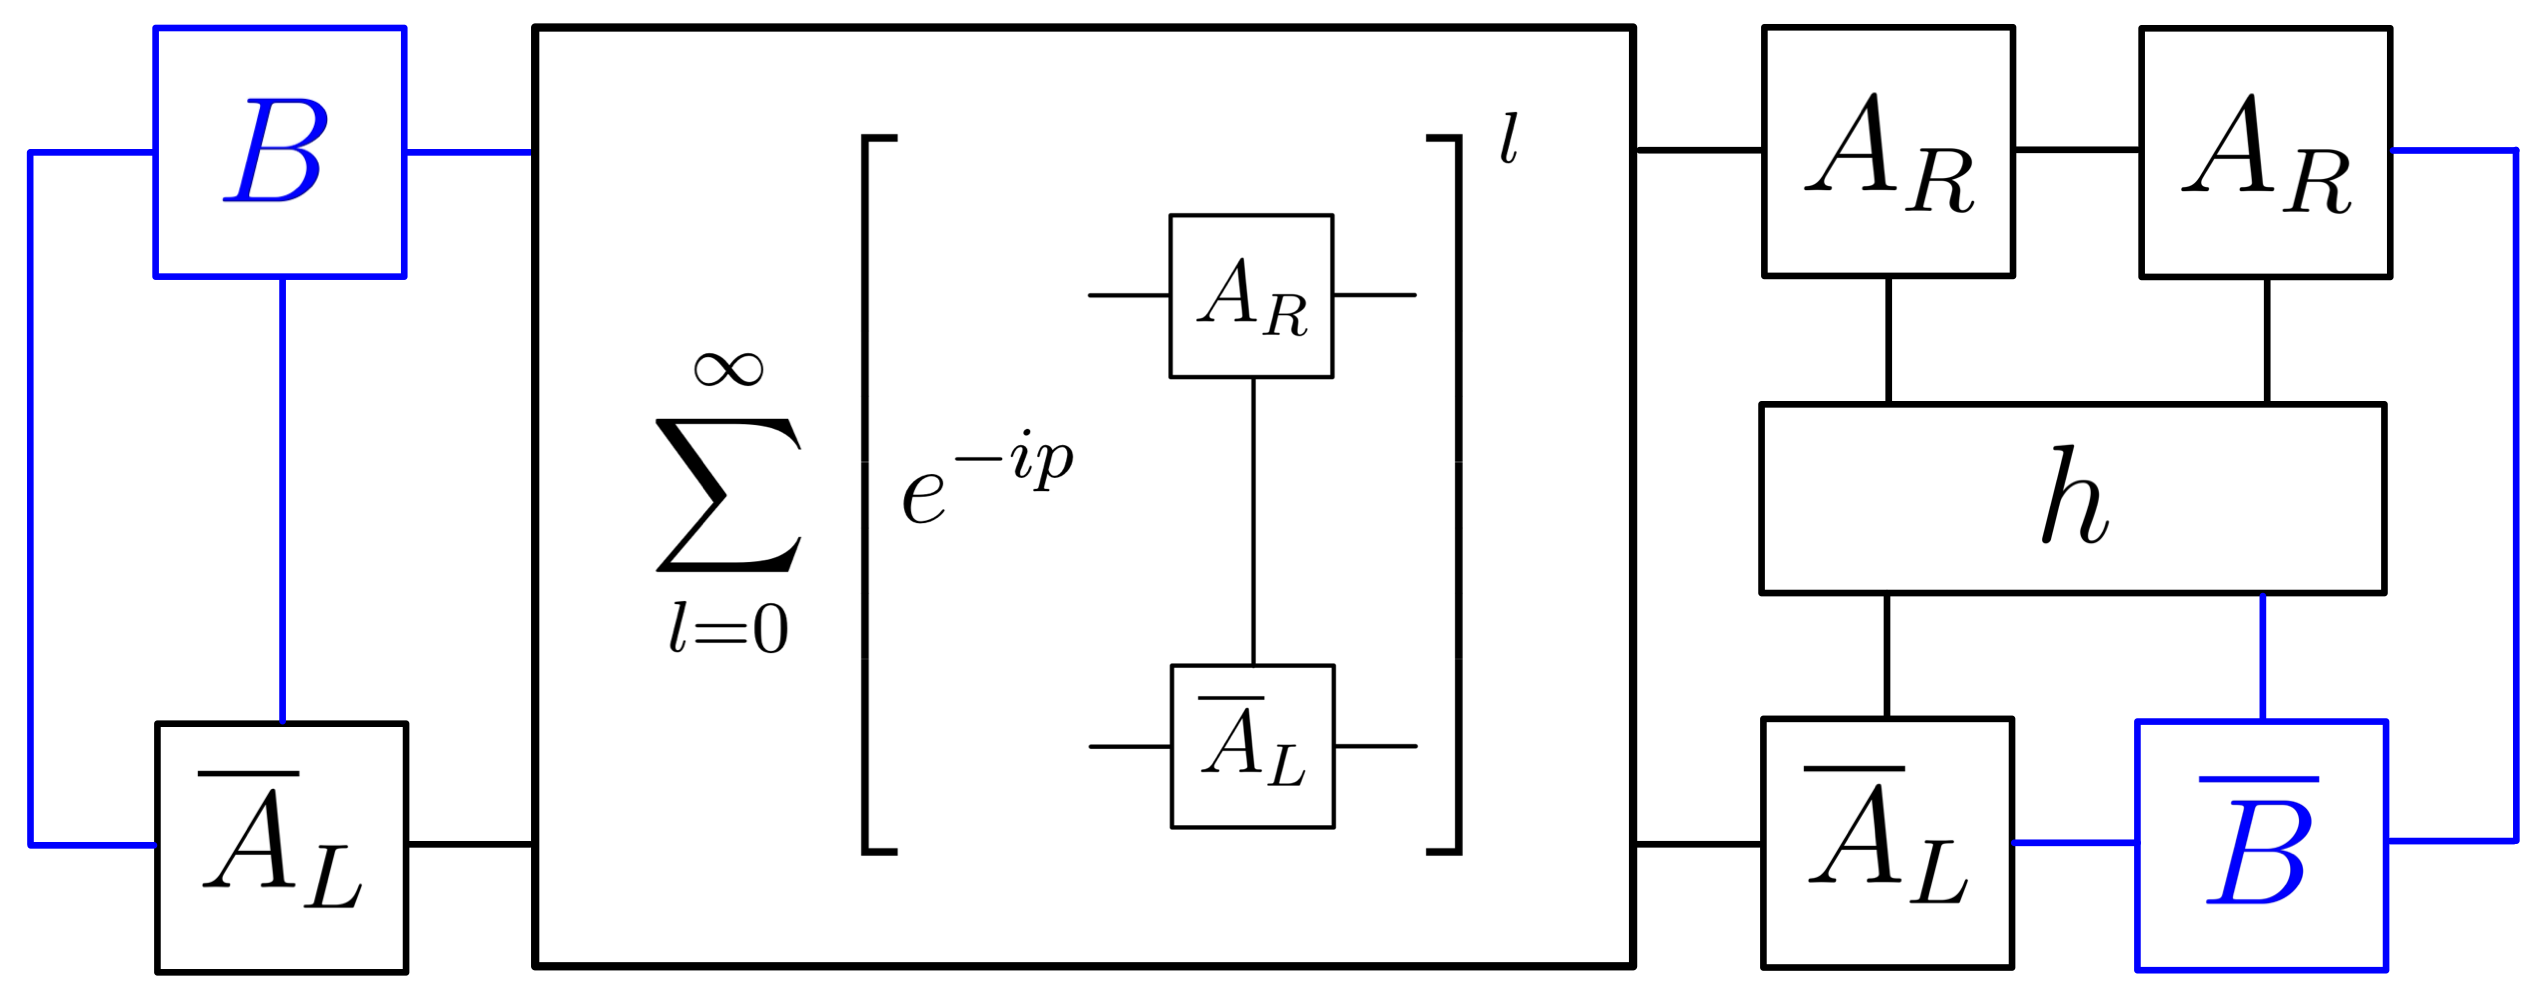
\includegraphics[height=3cm]{b6.png}}}_{=0}
\end{equation*}

\vspace{1em} 

1c) $n = 0$
\begin{equation*}
	\: + \: \underbrace{e^{-ip} 
	\raisebox{-0.5\height}{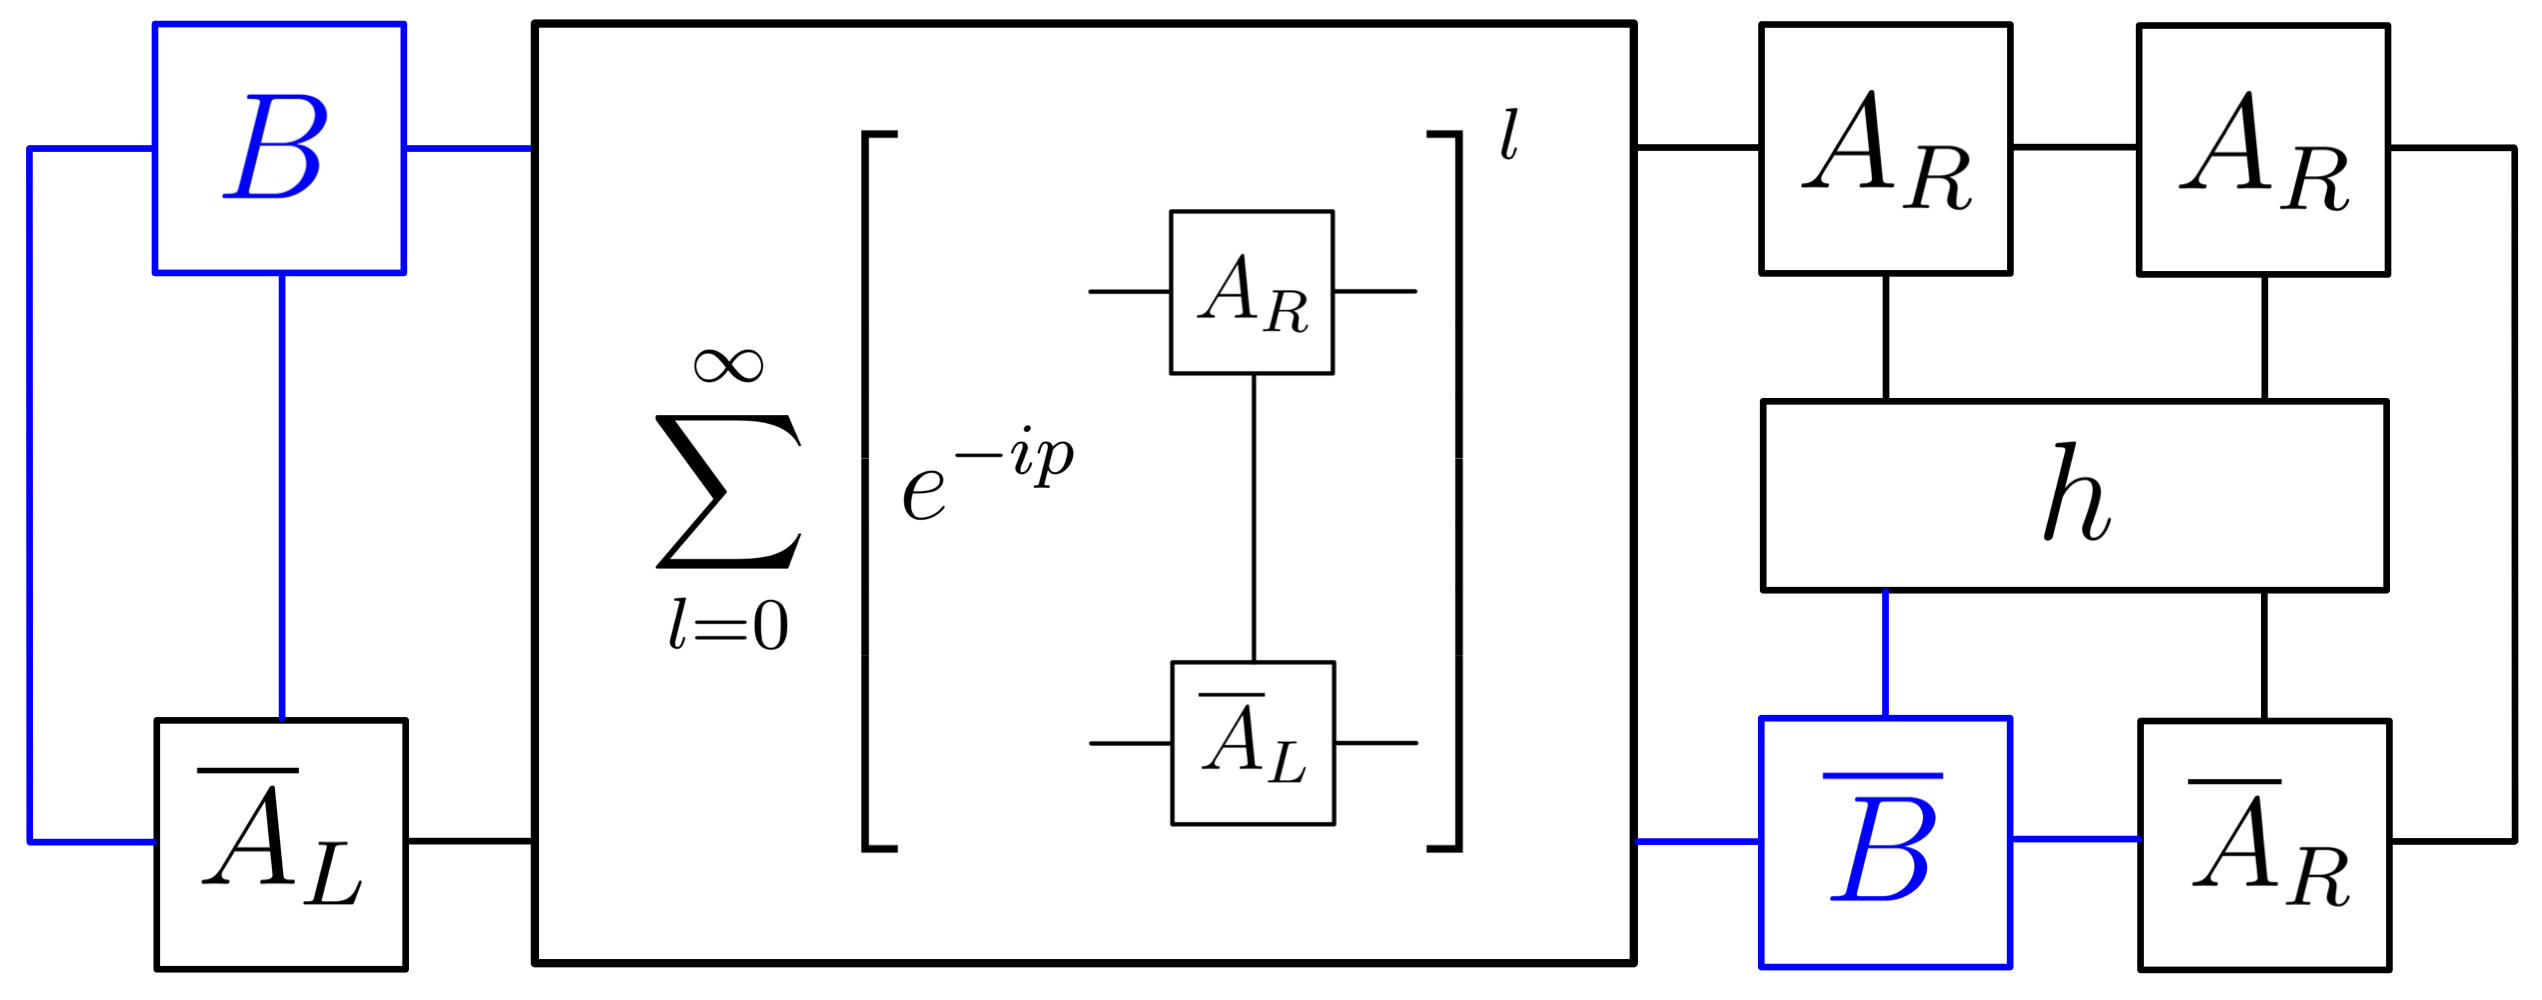
\includegraphics[height=3cm]{b7.png}}}_{=0}
\end{equation*}

\vspace{1em} 

1d) $n = 1, \ldots, \infty$
\begin{equation*}
	\: + \: \underbrace{e^{-ip} 
	\raisebox{-0.5\height}{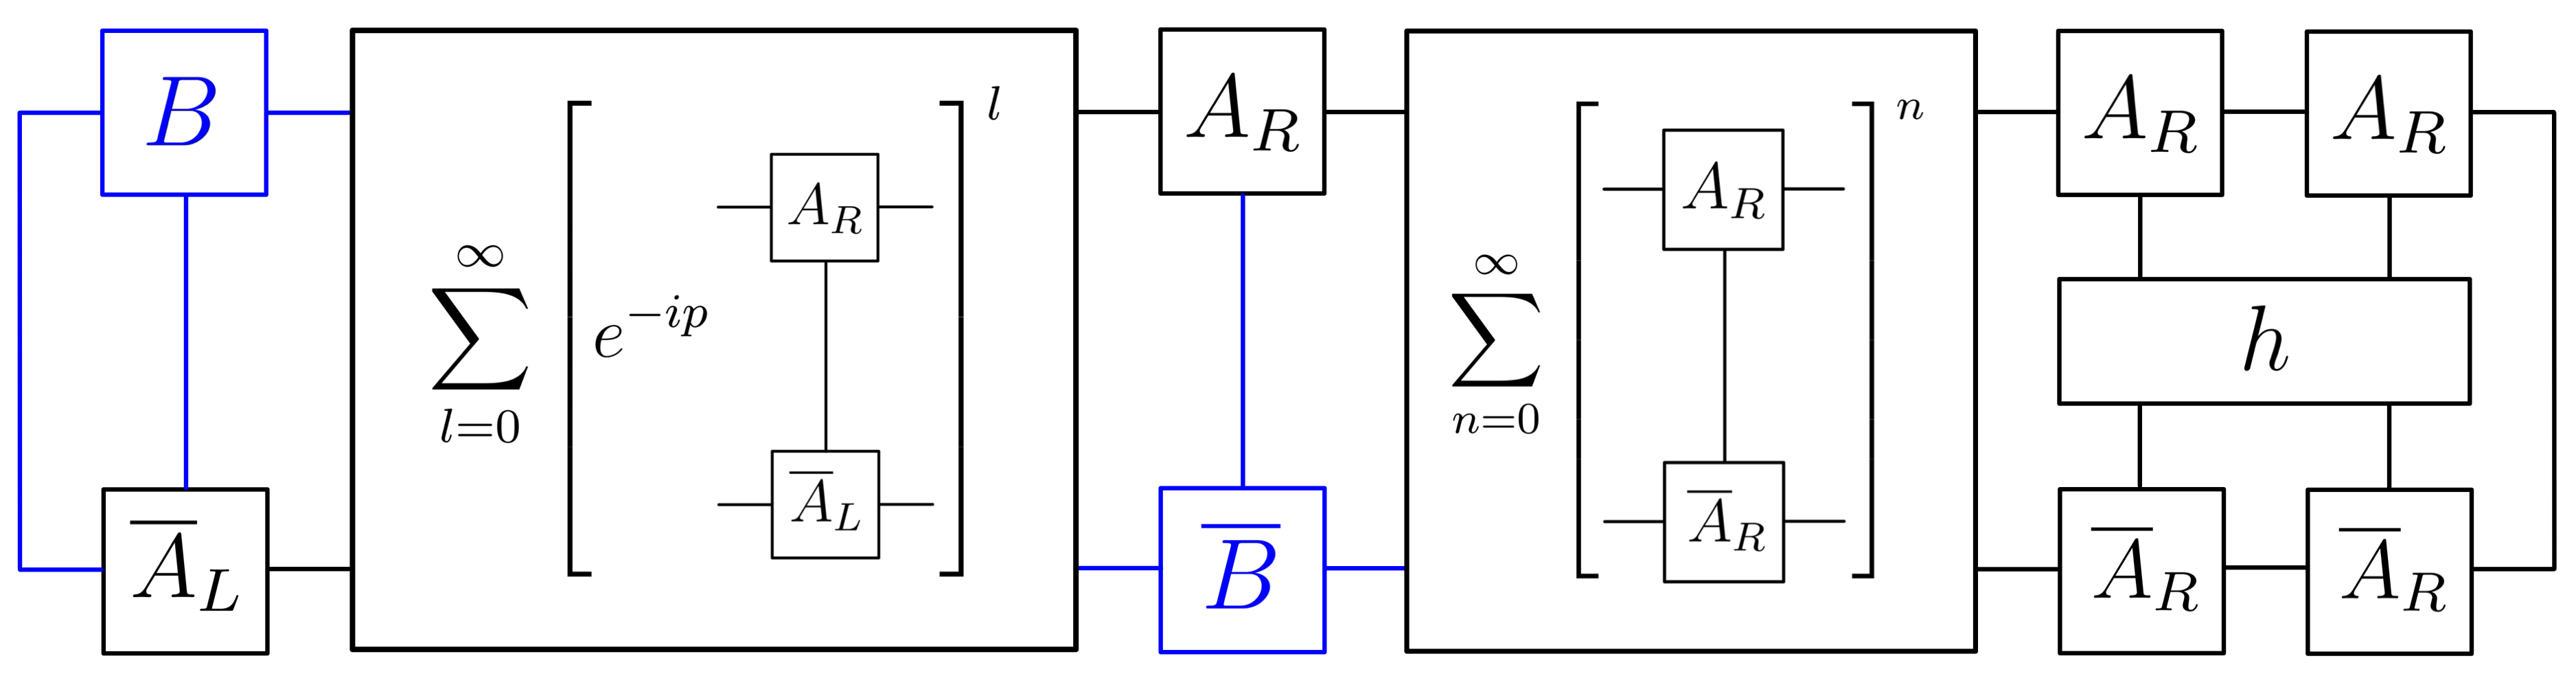
\includegraphics[height=3cm]{b8.png}}}_{=0}
\end{equation*}

\vspace{1em} 

2) $m = 0$

\vspace{1em} 

2a) $n = -2, \ldots, - \infty$ 
\begin{equation*}
	\: + \: 
	\raisebox{-0.5\height}{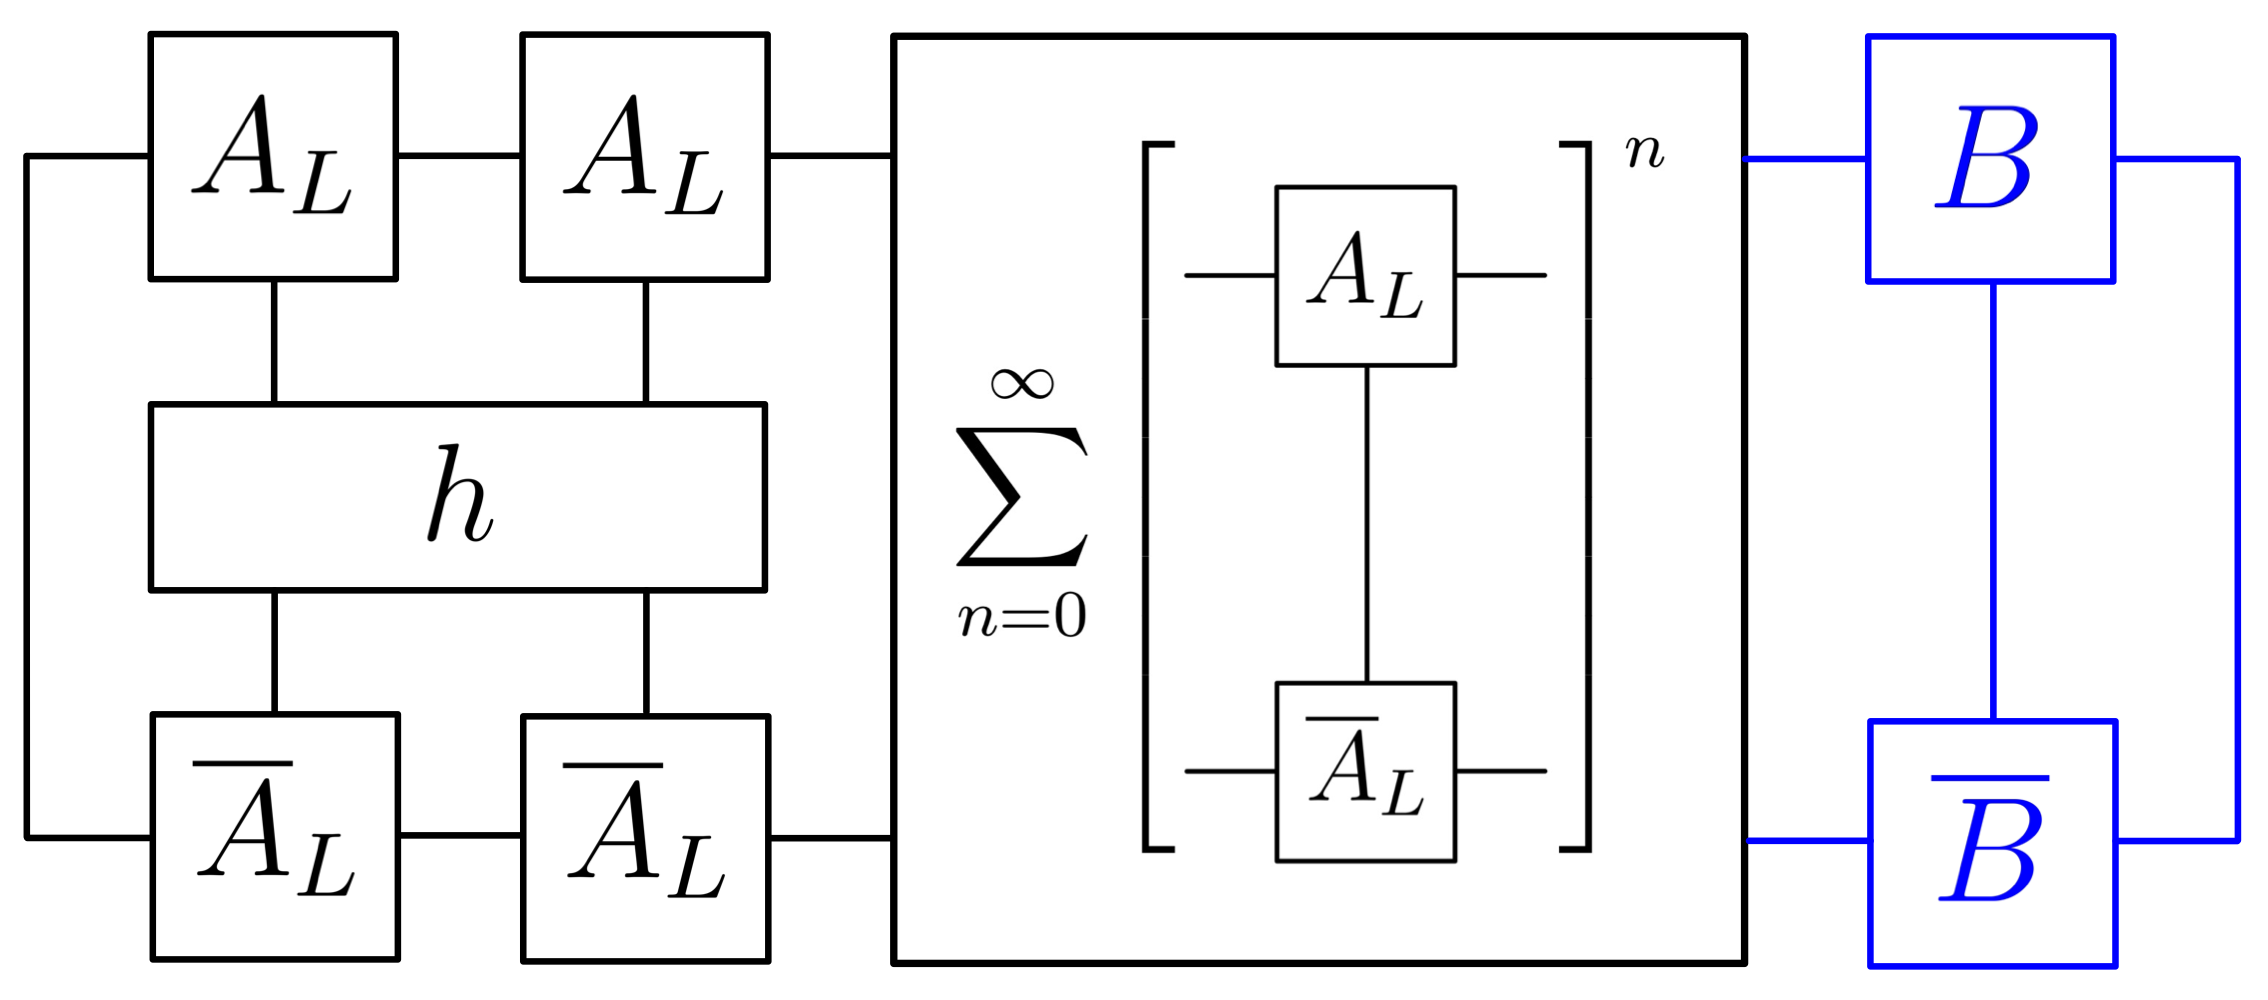
\includegraphics[height=3cm]{b9.png}} 
\end{equation*}

\vspace{1em} 

2b,c) $n = -1, 0$
\begin{equation*}
	\: + \: \raisebox{-0.5\height}{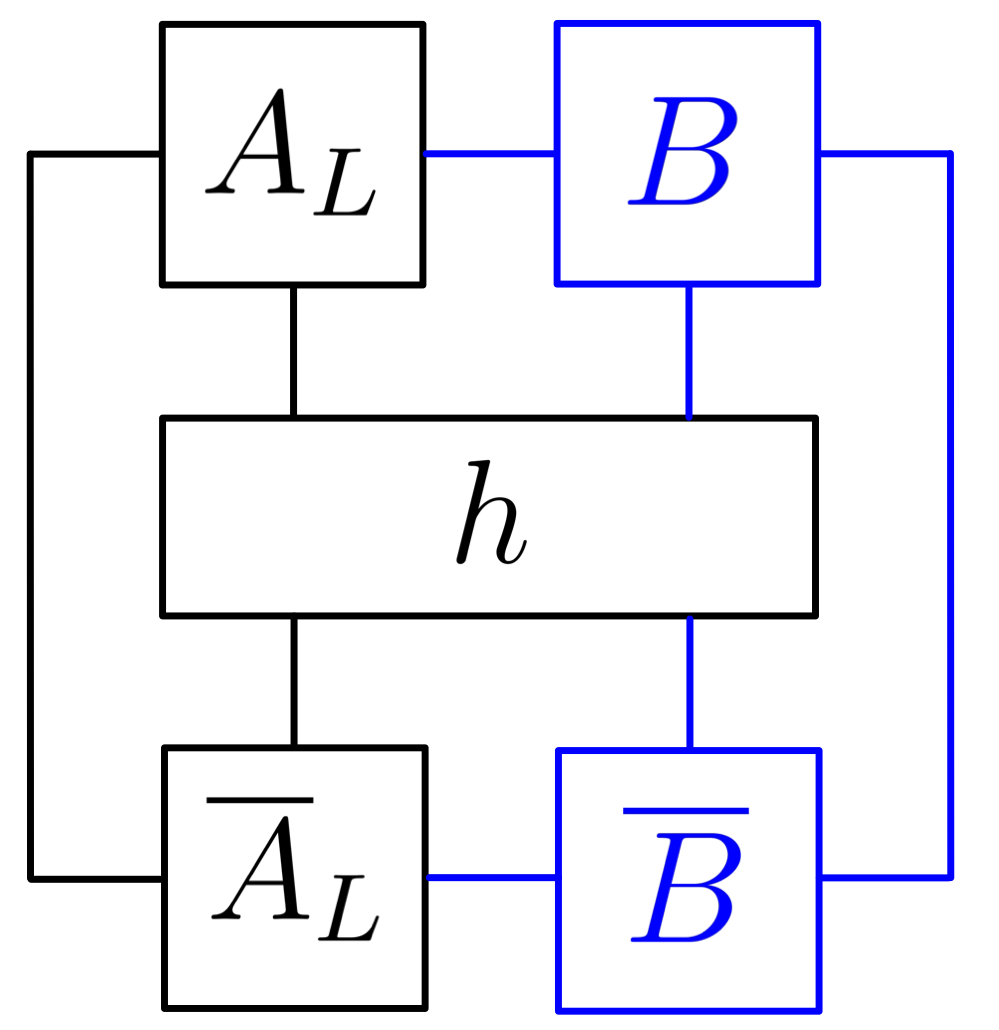
\includegraphics[height=3cm]{b10.png}}
	\: + \: \raisebox{-0.5\height}{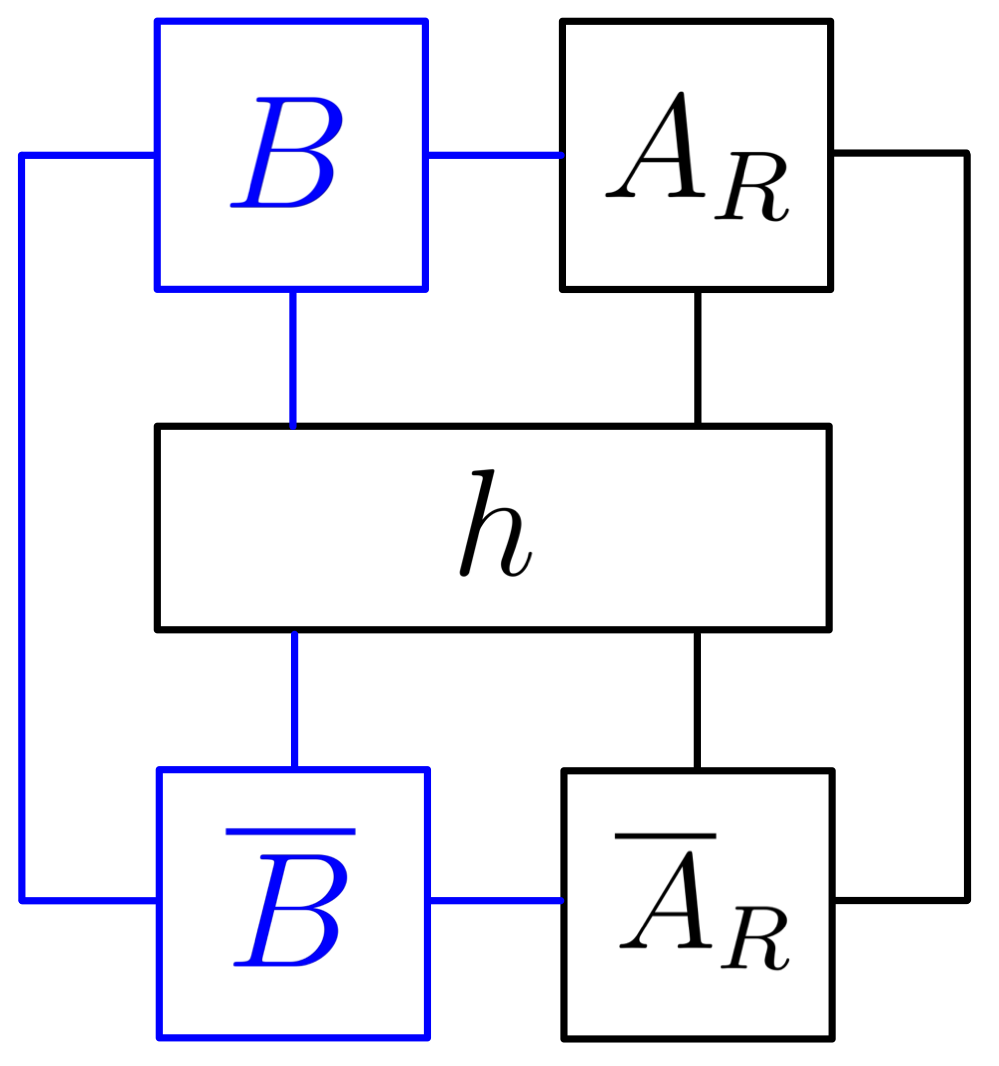
\includegraphics[height=3cm]{b11.png}}
\end{equation*}

\vspace{1em} 

2d) $n = 1, \ldots, \infty$
\begin{equation*}
	\: + \: 
	\raisebox{-0.5\height}{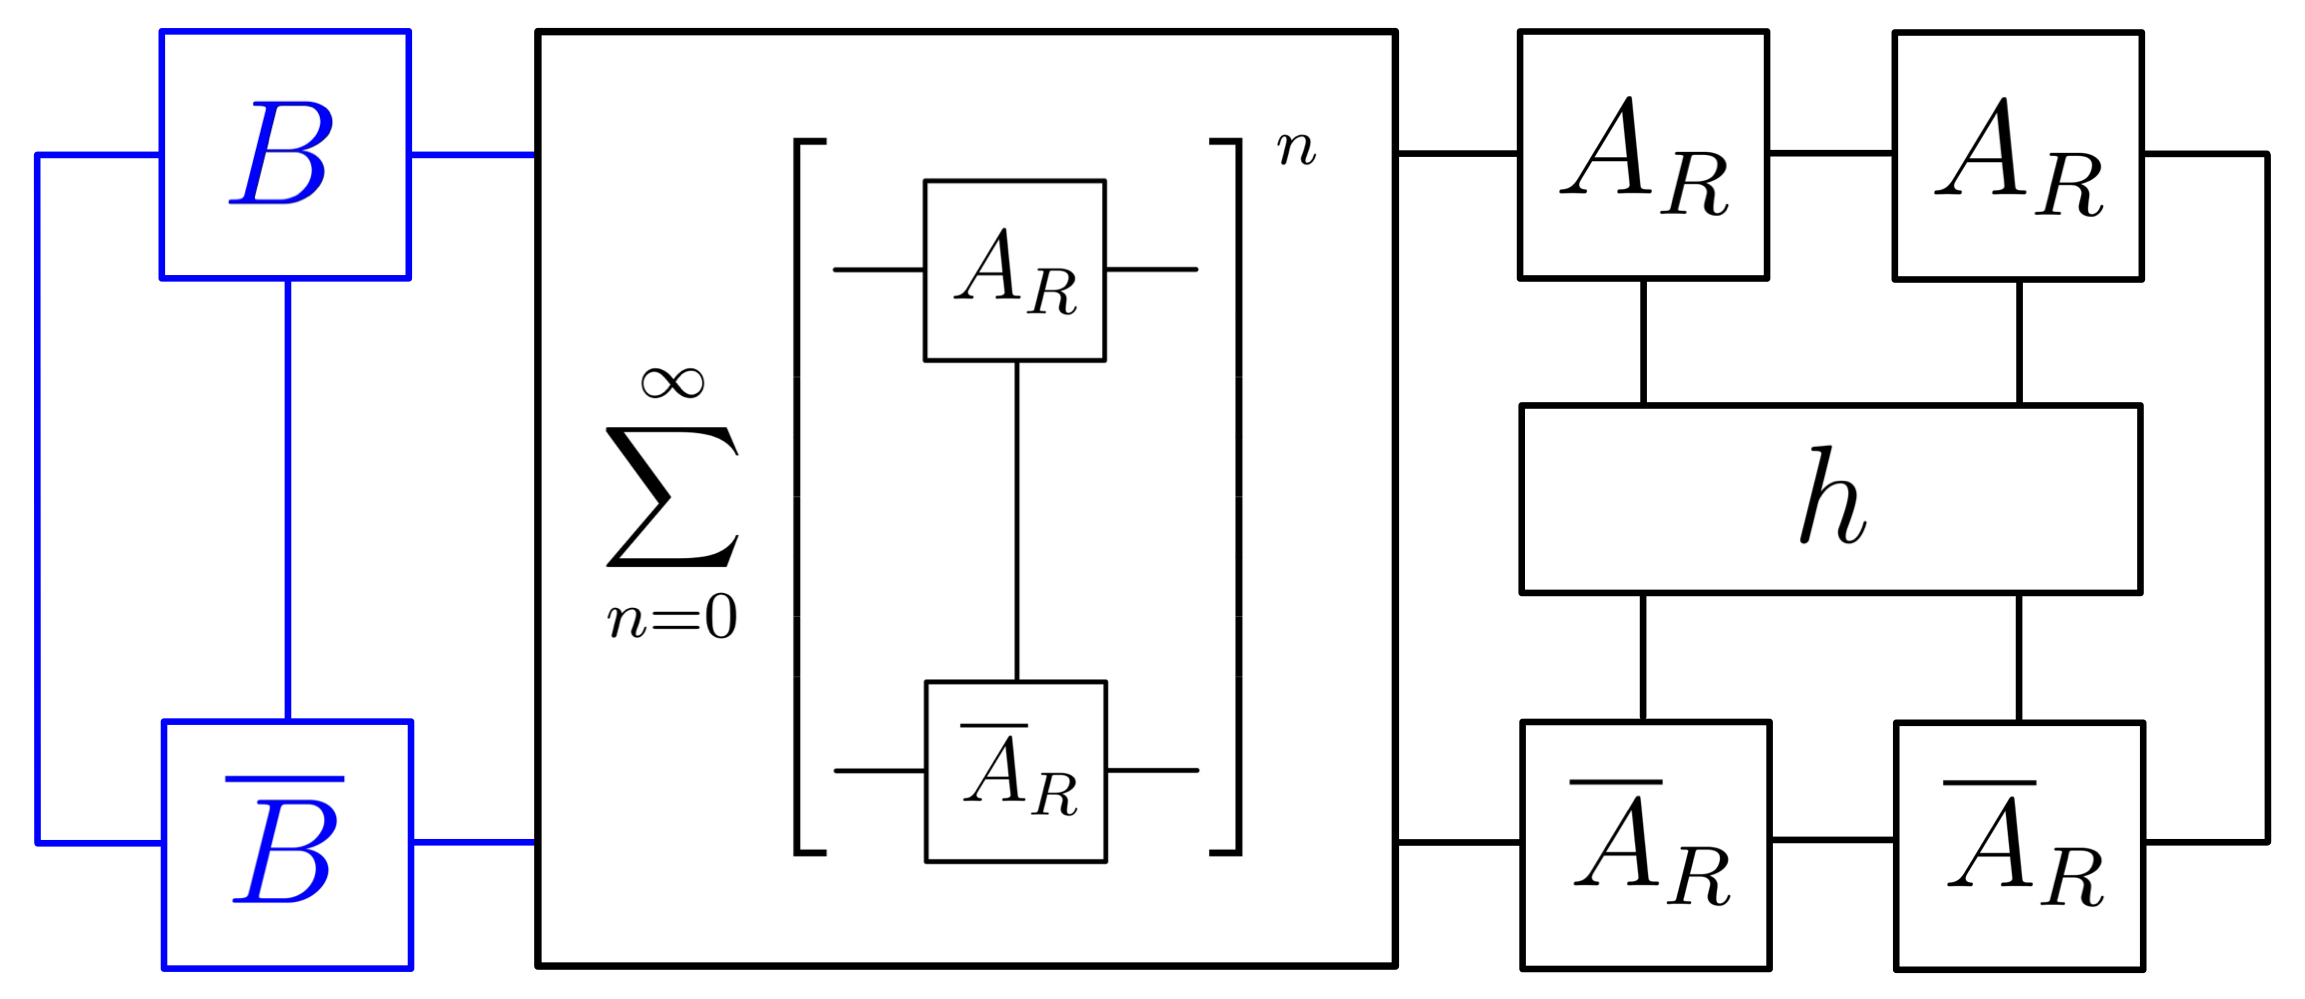
\includegraphics[height=3cm]{b12.png}}  
\end{equation*}

3) $m = 1, \ldots, \infty$

\vspace{1em} 

3a) $n = -2, \ldots, - \infty$
\begin{equation*}
	\: + \: e^{ip} 
	\raisebox{-0.5\height}{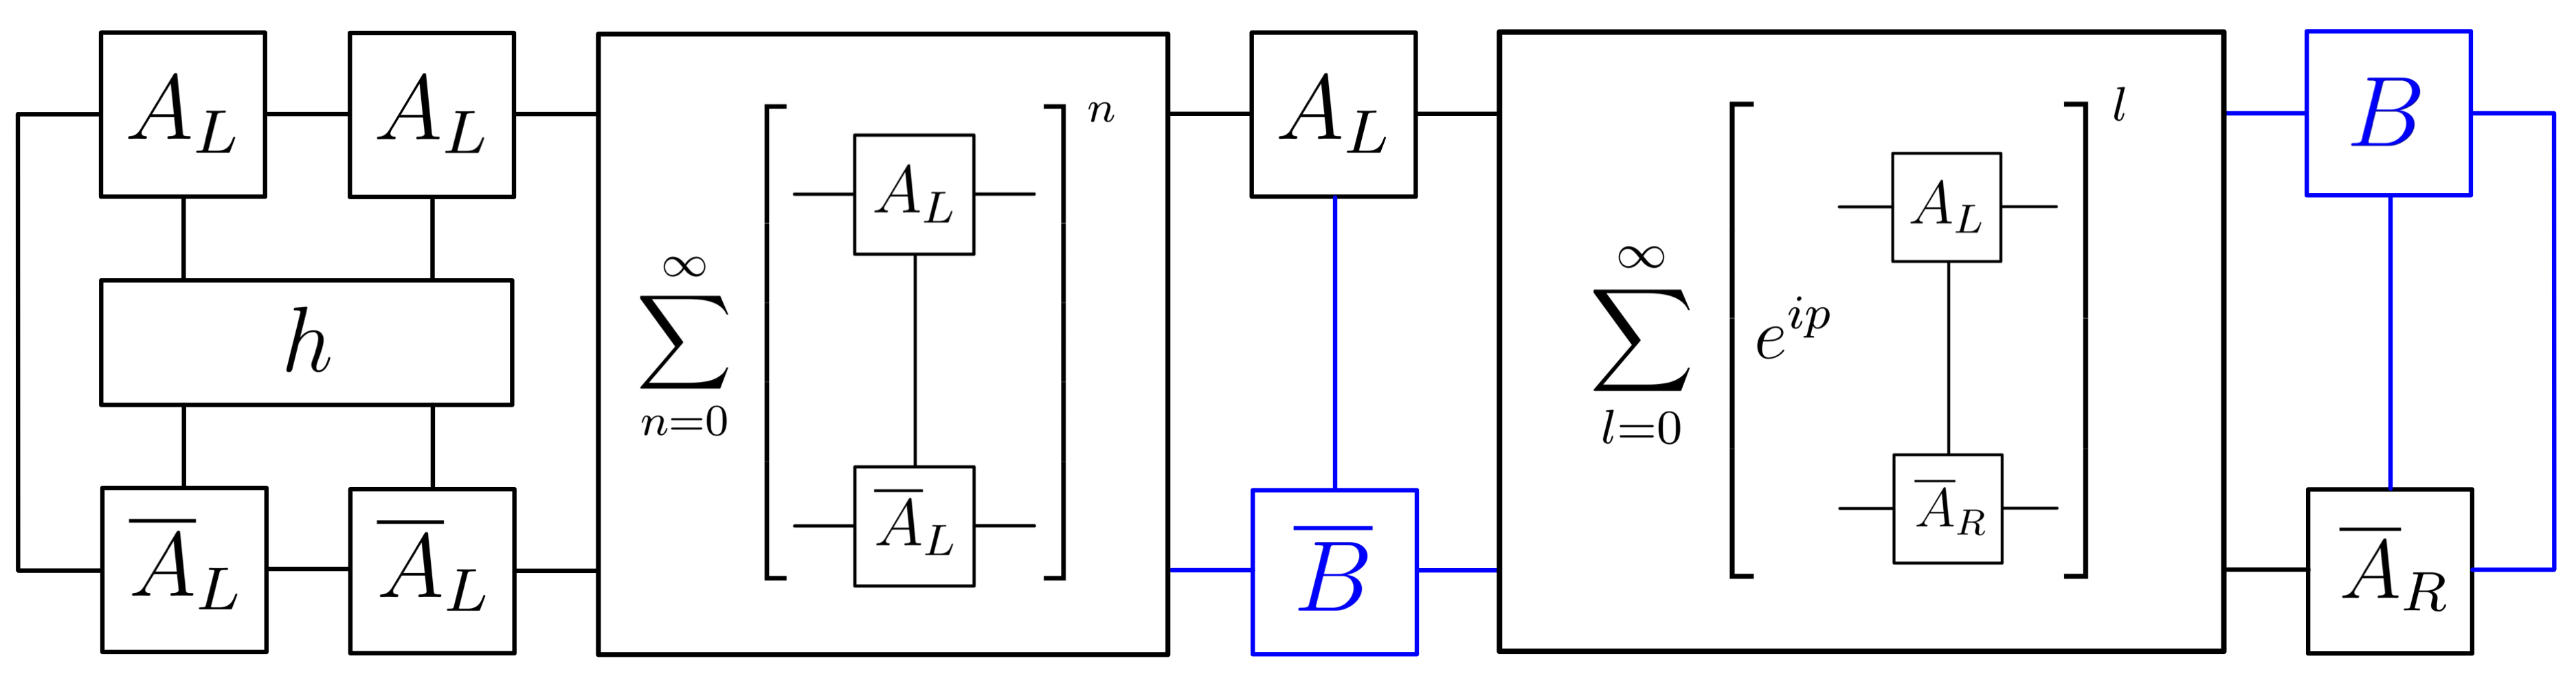
\includegraphics[height=3cm]{b13.png}} 
\end{equation*}

\vspace{1em} 

3b) $n = -1$
\begin{equation*}
	\: + \: e^{ip}
	\raisebox{-0.5\height}{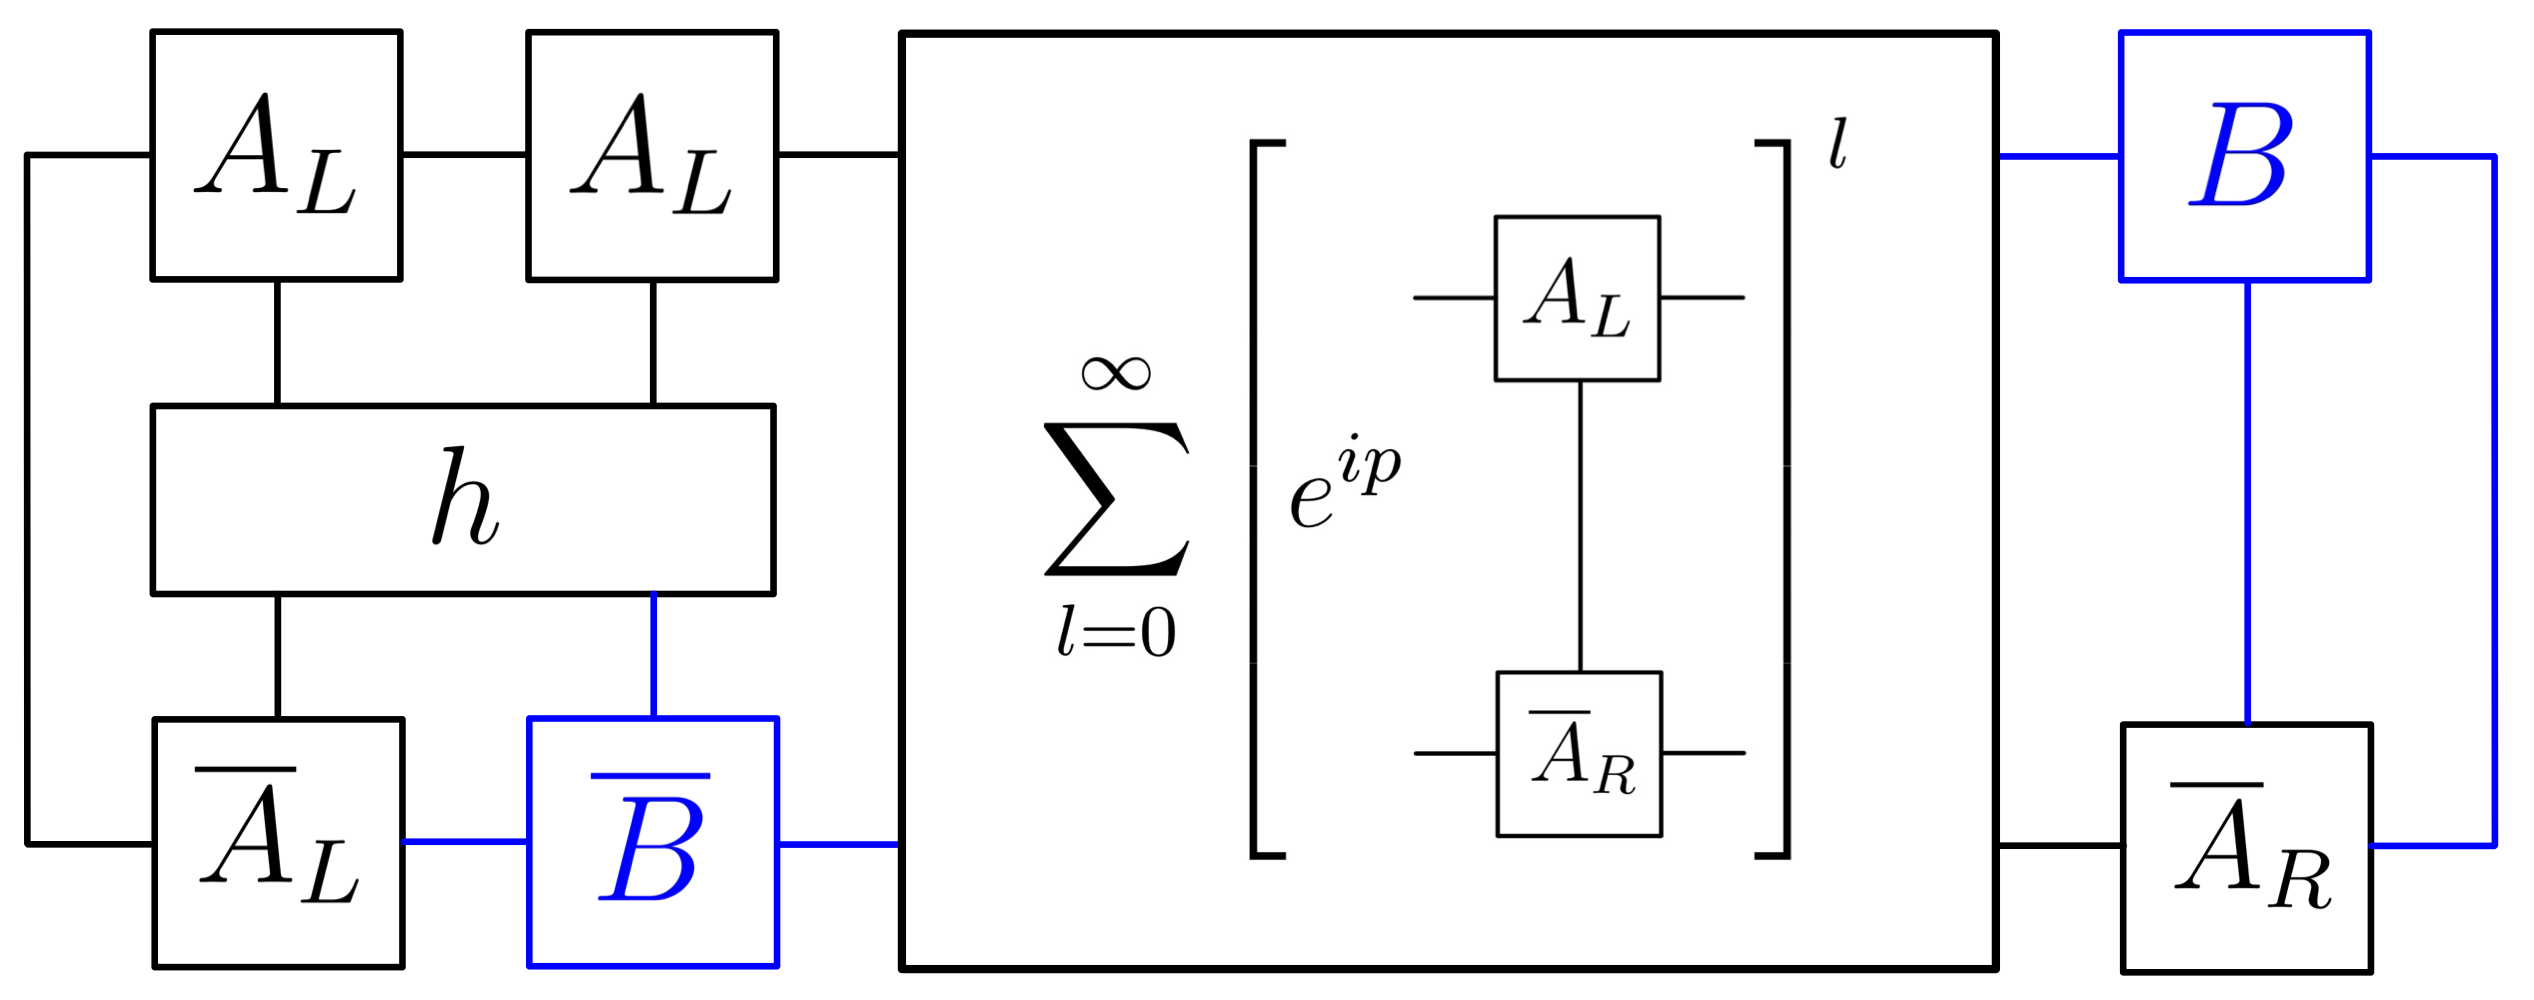
\includegraphics[height=3cm]{b14.png}}
\end{equation*}

\vspace{1em} 

3c) $n = 0$
\begin{equation*}
	\: + \: 
	e^{ip}
	\raisebox{-0.5\height}{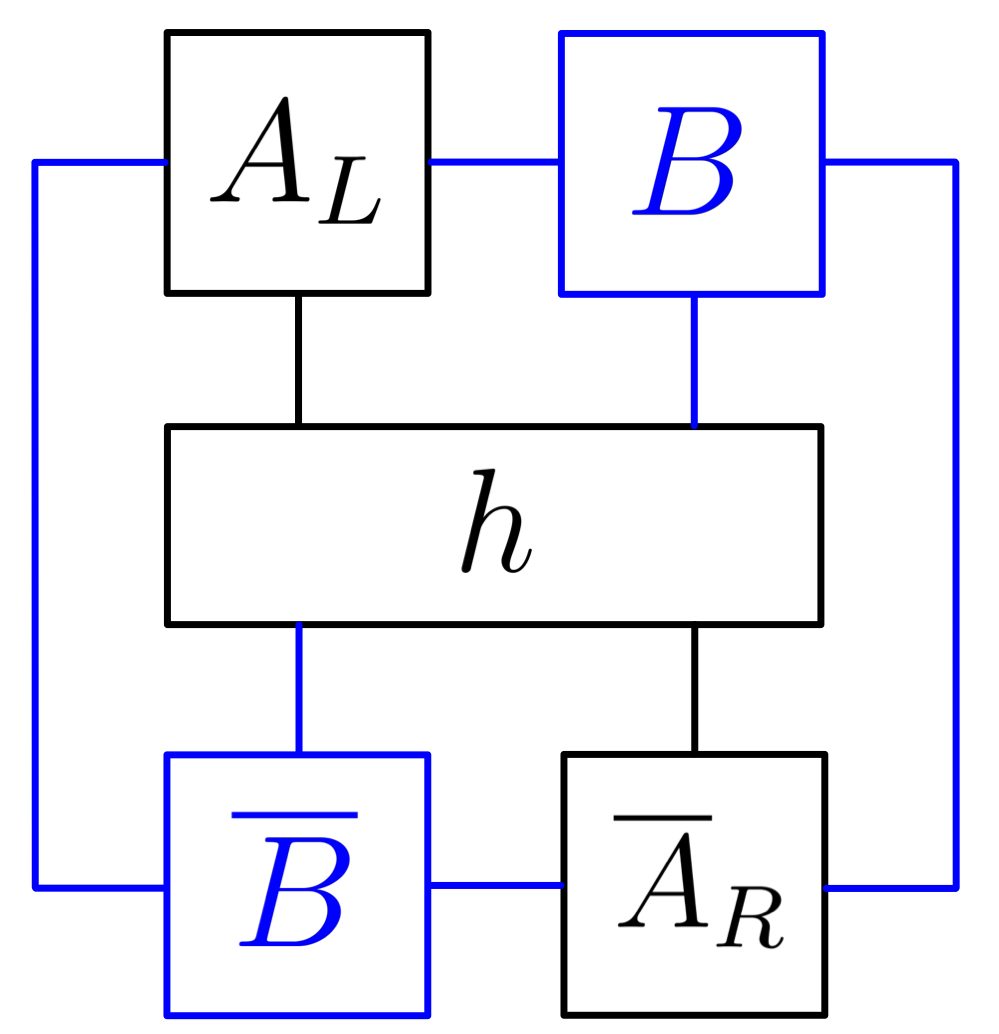
\includegraphics[height=3cm]{b15.png}}
	\: + \: 
	e^{2ip}
	\raisebox{-0.5\height}{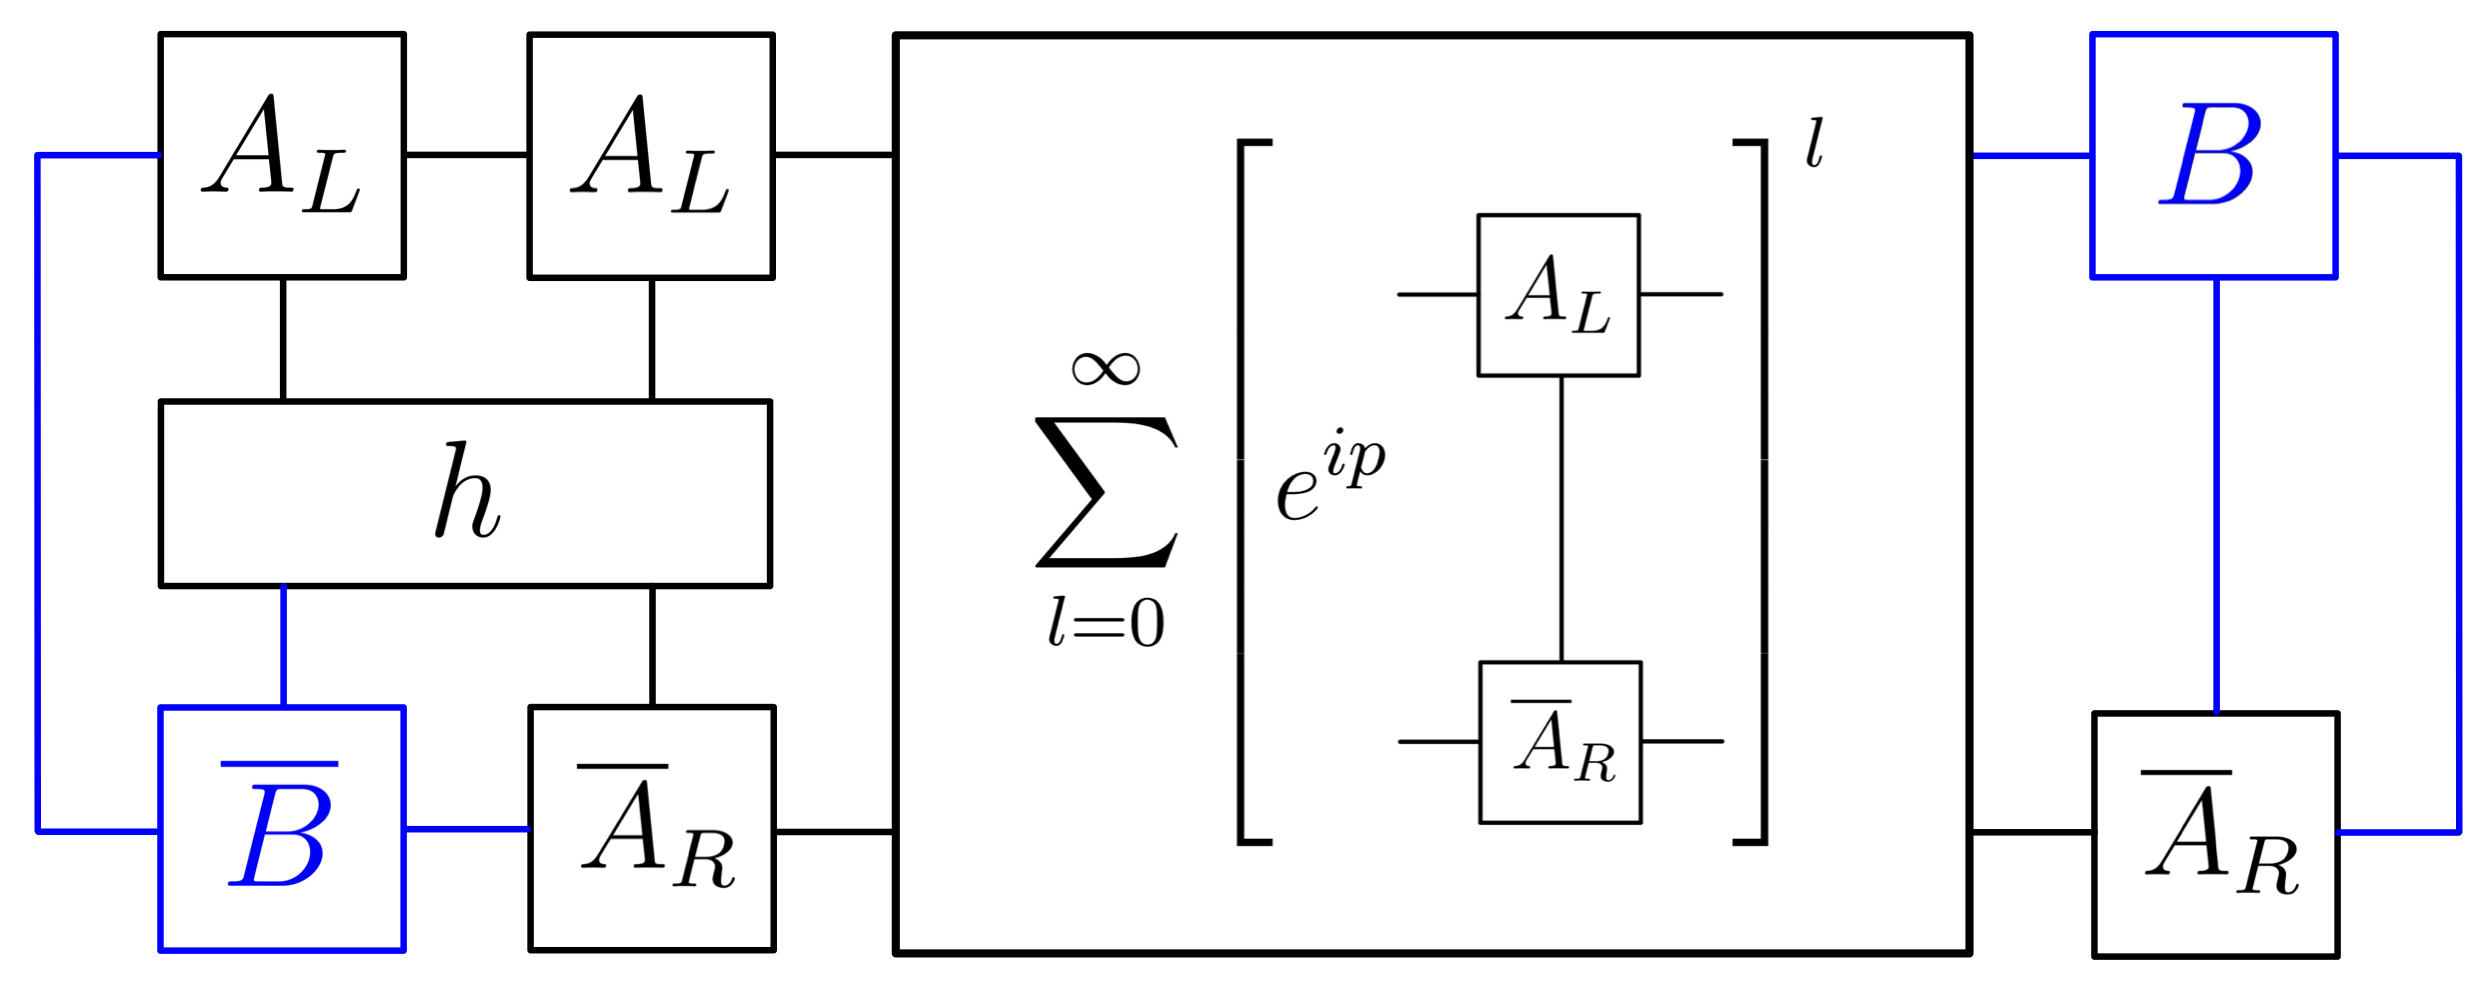
\includegraphics[height=3cm]{b16.png}}
\end{equation*}

\vspace{1em} 

3d) $n = 1, \ldots, \infty$
\begin{equation*}
	\: + \: \underbrace{e^{ip}
	\raisebox{-0.5\height}{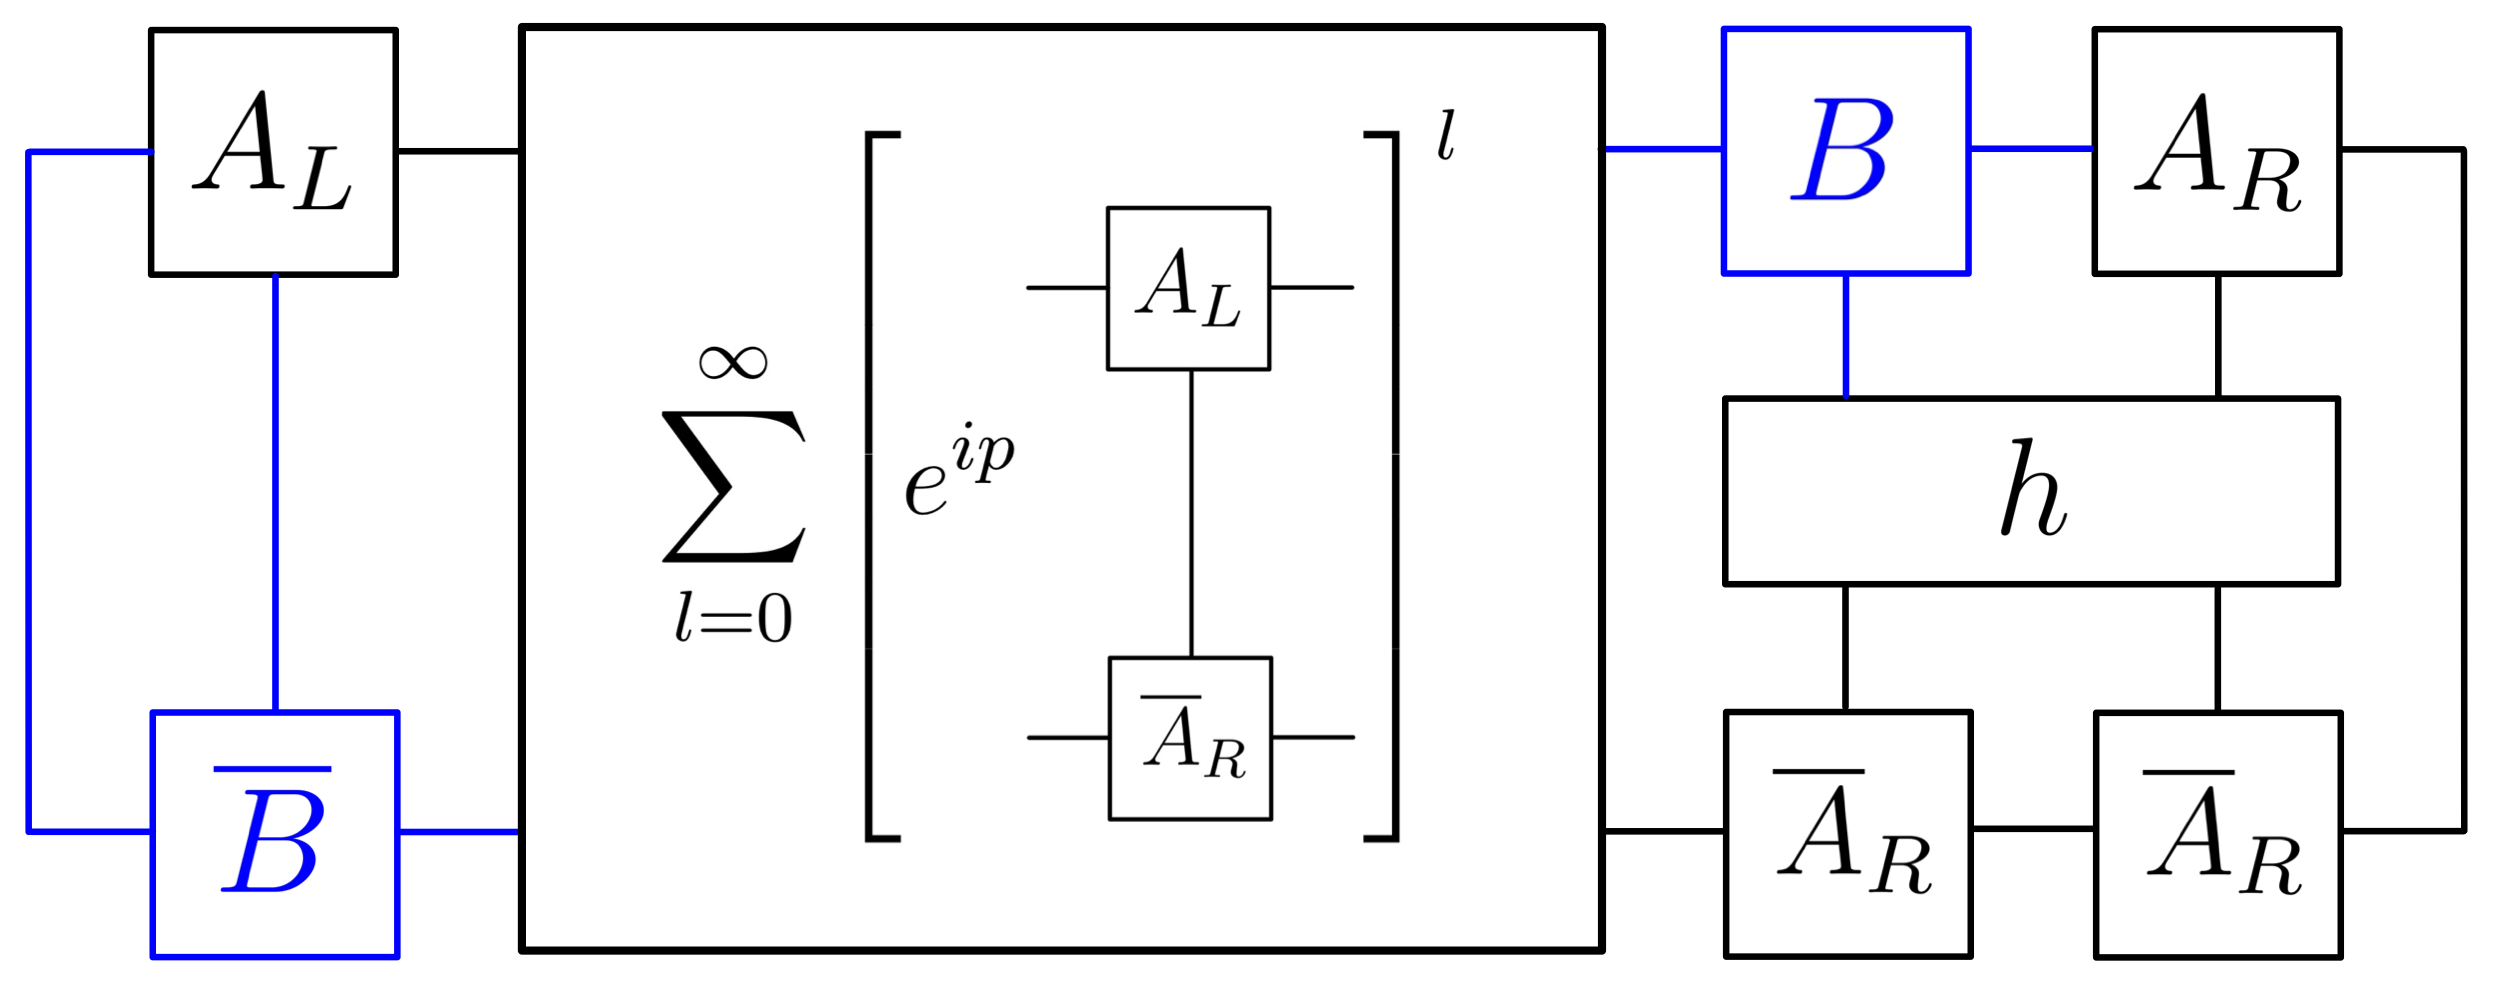
\includegraphics[height=3cm]{b17.png}}}_{= 0}
	\: + \: \underbrace{e^{2ip}
	\raisebox{-0.5\height}{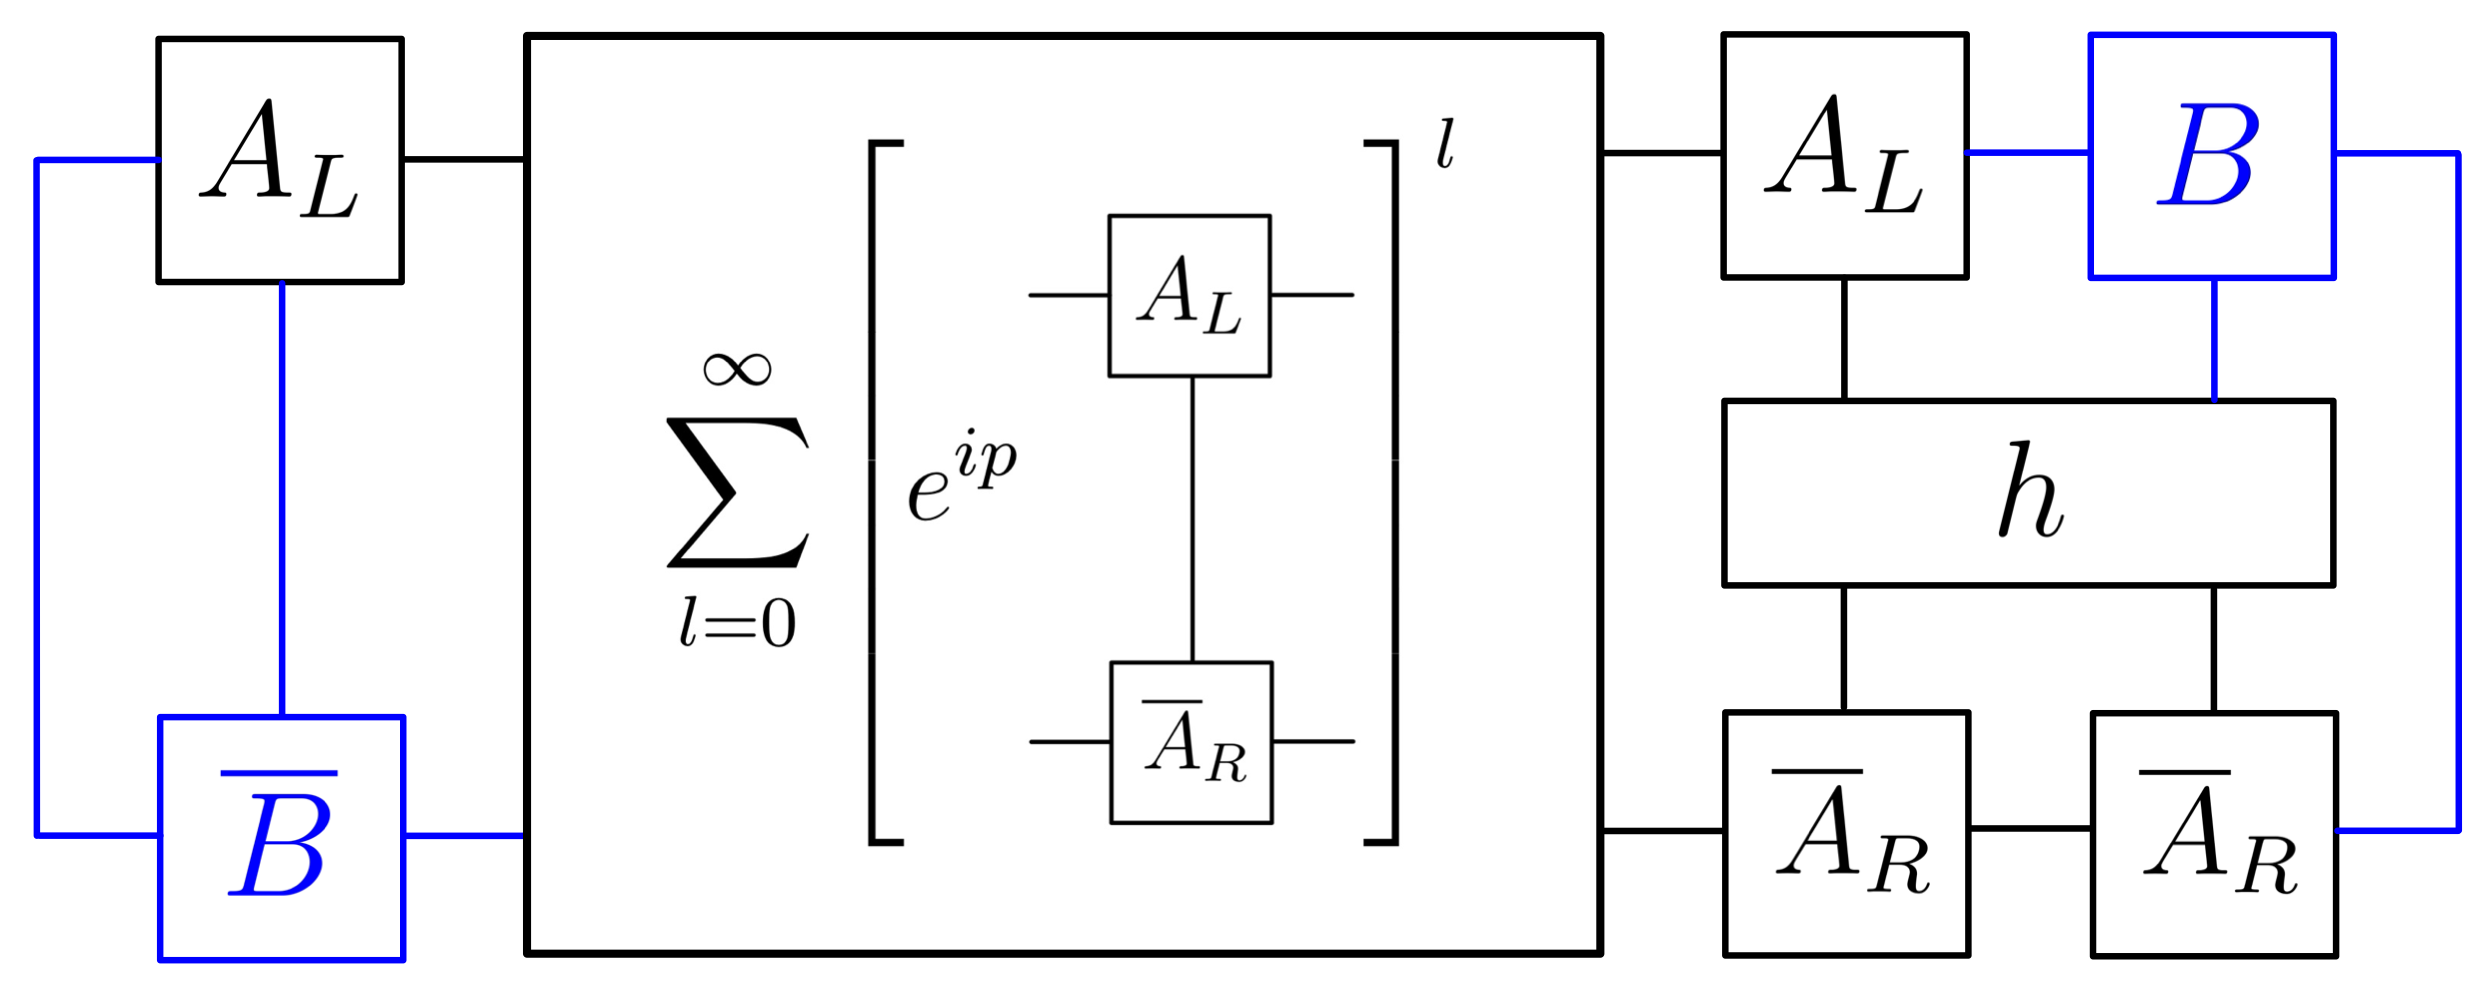
\includegraphics[height=3cm]{b18.png}}}_{= 0}
\end{equation*}
\begin{equation*}
	\: + \: \underbrace{e^{3ip}
	\raisebox{-0.5\height}{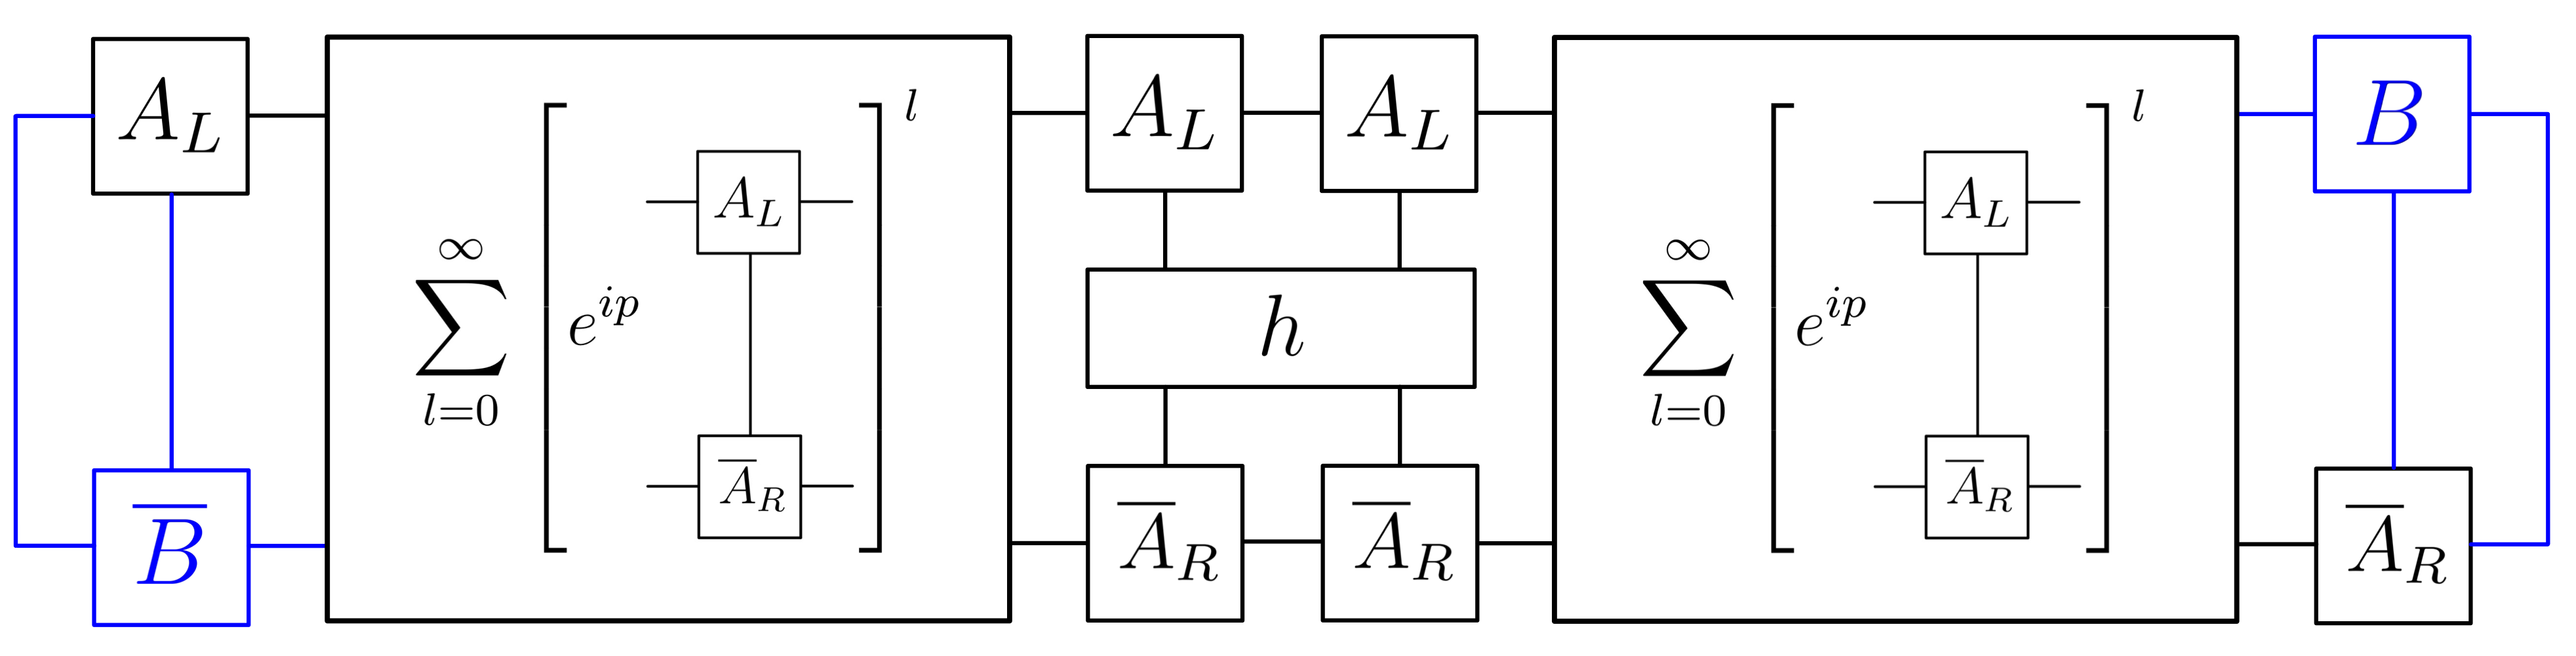
\includegraphics[height=3cm]{b19.png}}}_{= 0}
\end{equation*}
\begin{equation*}
	\: + \: \underbrace{e^{ip}
	\raisebox{-0.5\height}{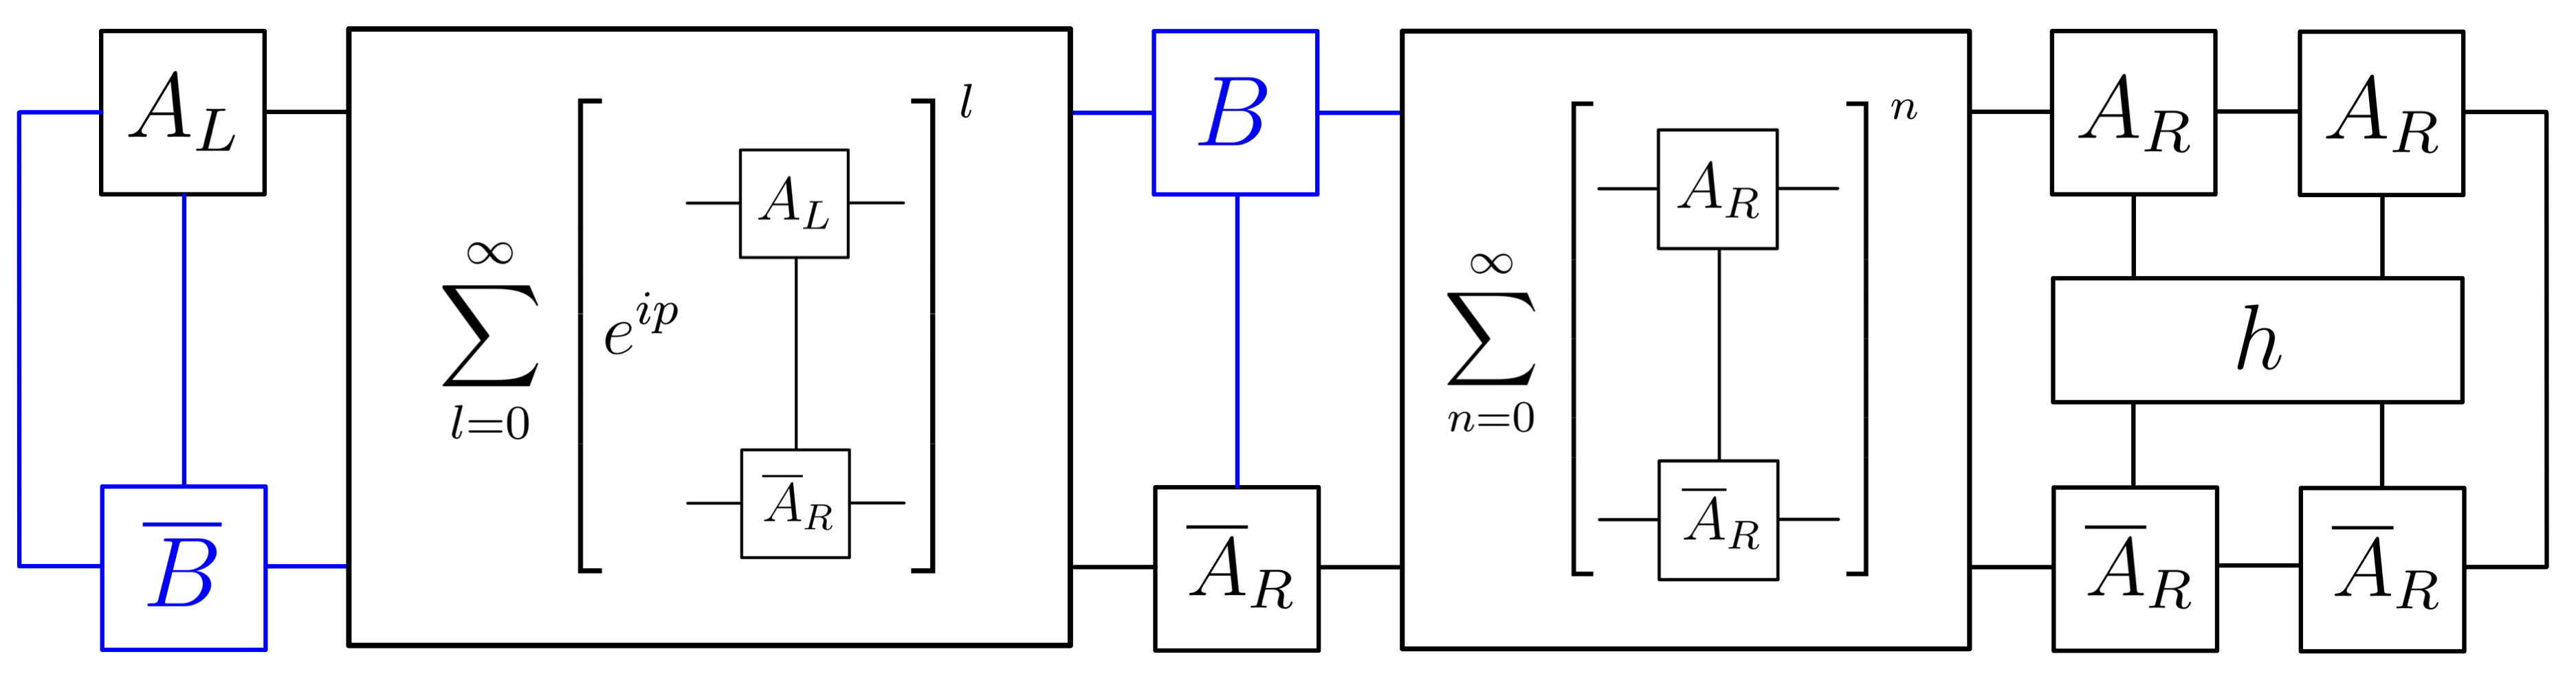
\includegraphics[height=3cm]{b20.png}}}_{= 0}
\end{equation*}
\end{center}


% EFFECTIVE TRANSLATION OPERATOR
% Teff
\newpage
\section*{Effective translation operator for MPS quasiparticle excitations}
For an MPS quasiparticle excitation ansatz \eqref{eq:emps_X}, variational in both energy and momentum, we have to solve the eigenvalue problem
\begin{equation*}
	\left[ H_{\text{eff}} - \alpha \left( e^{-i \frac{2\pi}{N}k} T_{\text{eff}} + e^{i \frac{2\pi}{N}k} T_{\text{eff}}^{\dagger} \right) \right] 
	 \tket{B} 
	 = \epsilon_k \tket{B}.
\end{equation*}
In this appendix we specify the boundary tensors for the effective translation operator $T_{\text{eff}}$ and its adjoint. Note that $B^{[n]} = V_L^{[n]} X^{[n]}$ \eqref{eq:excitation_gauge}. \\[1.5em]

\begin{align*}
\begin{split}
	\textcolor{blue}{\tbra{\overline{B}}} &T_{\text{eff}} \textcolor{blue}{\tket{B}} \\
	&=
\end{split}
\end{align*}
\vspace*{-0.5cm}
\begin{equation*}
	\raisebox{-0.45\height}{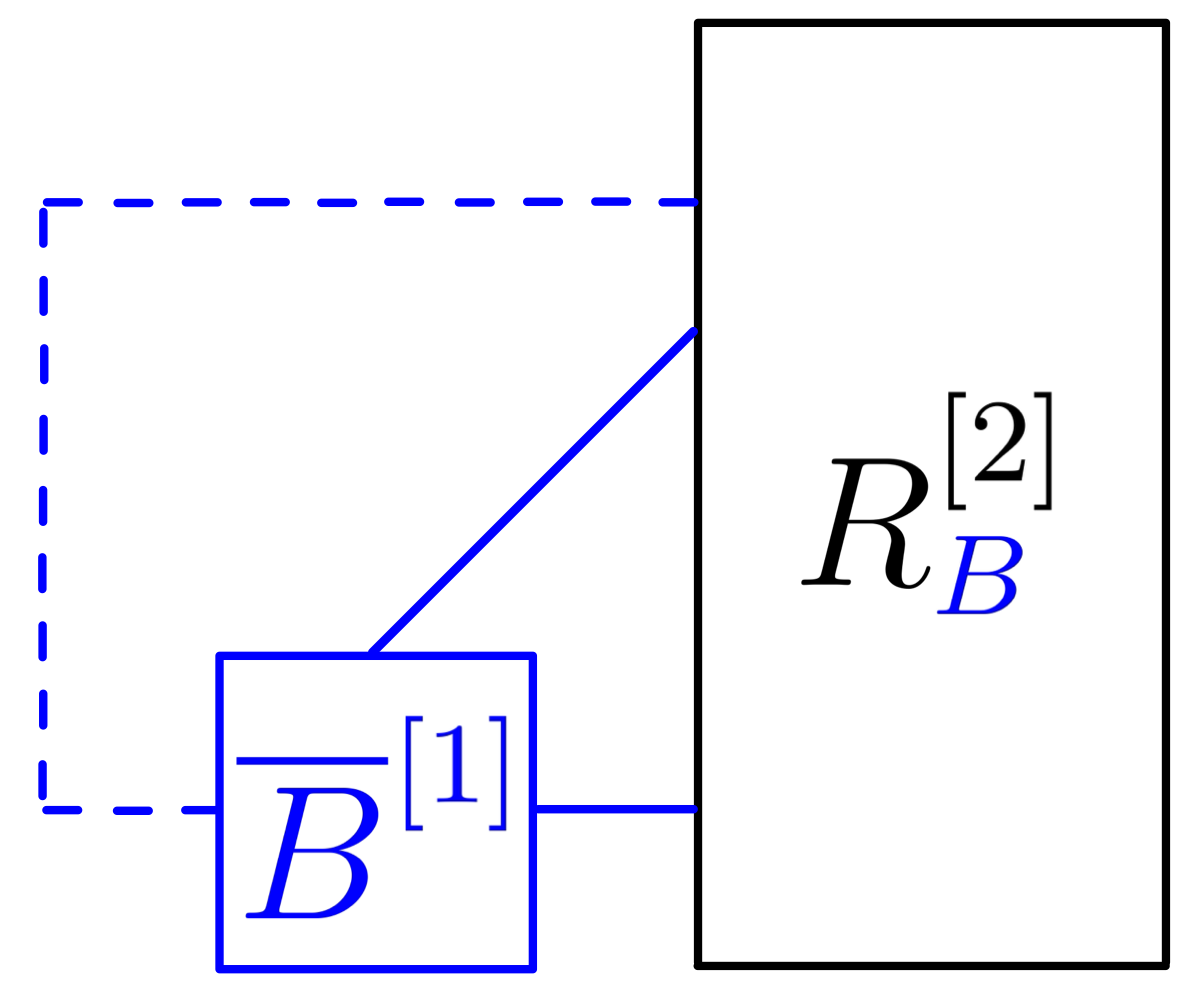
\includegraphics[height=2.cm]{T1.png}} 
	\:+\: \sum_{n=2}^N \left[
	\raisebox{-0.45\height}{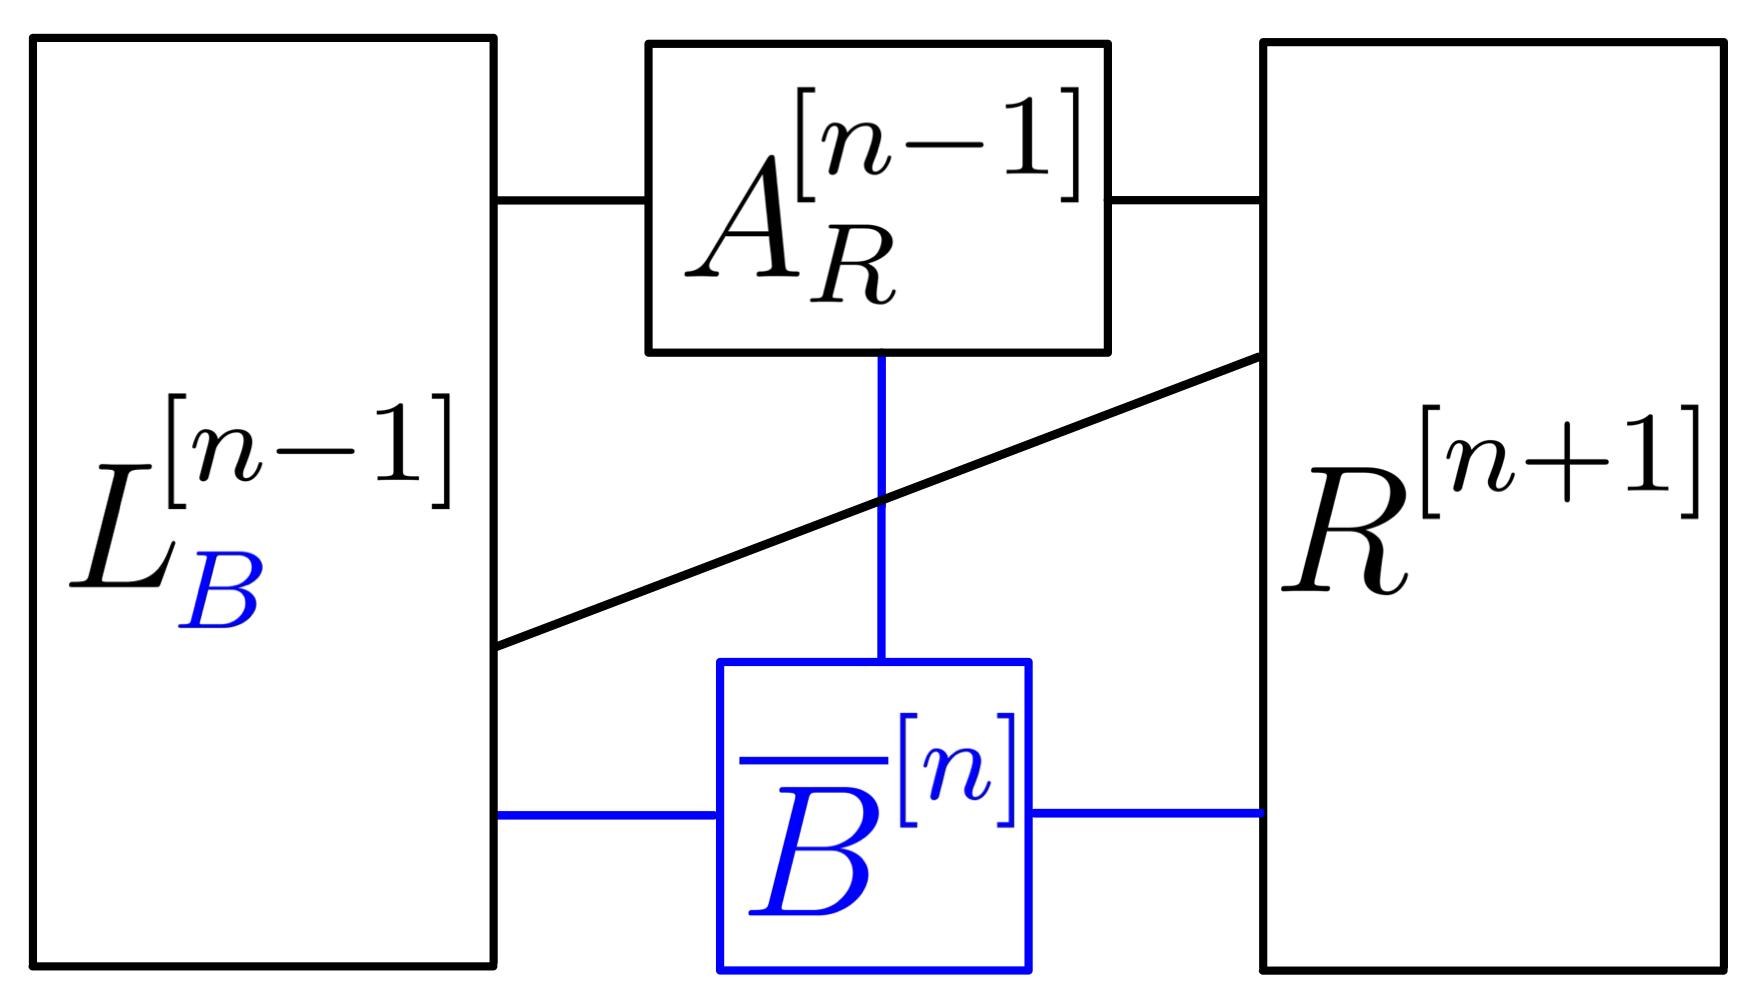
\includegraphics[height=2.cm]{T2.png}}
	+
	\raisebox{-0.45\height}{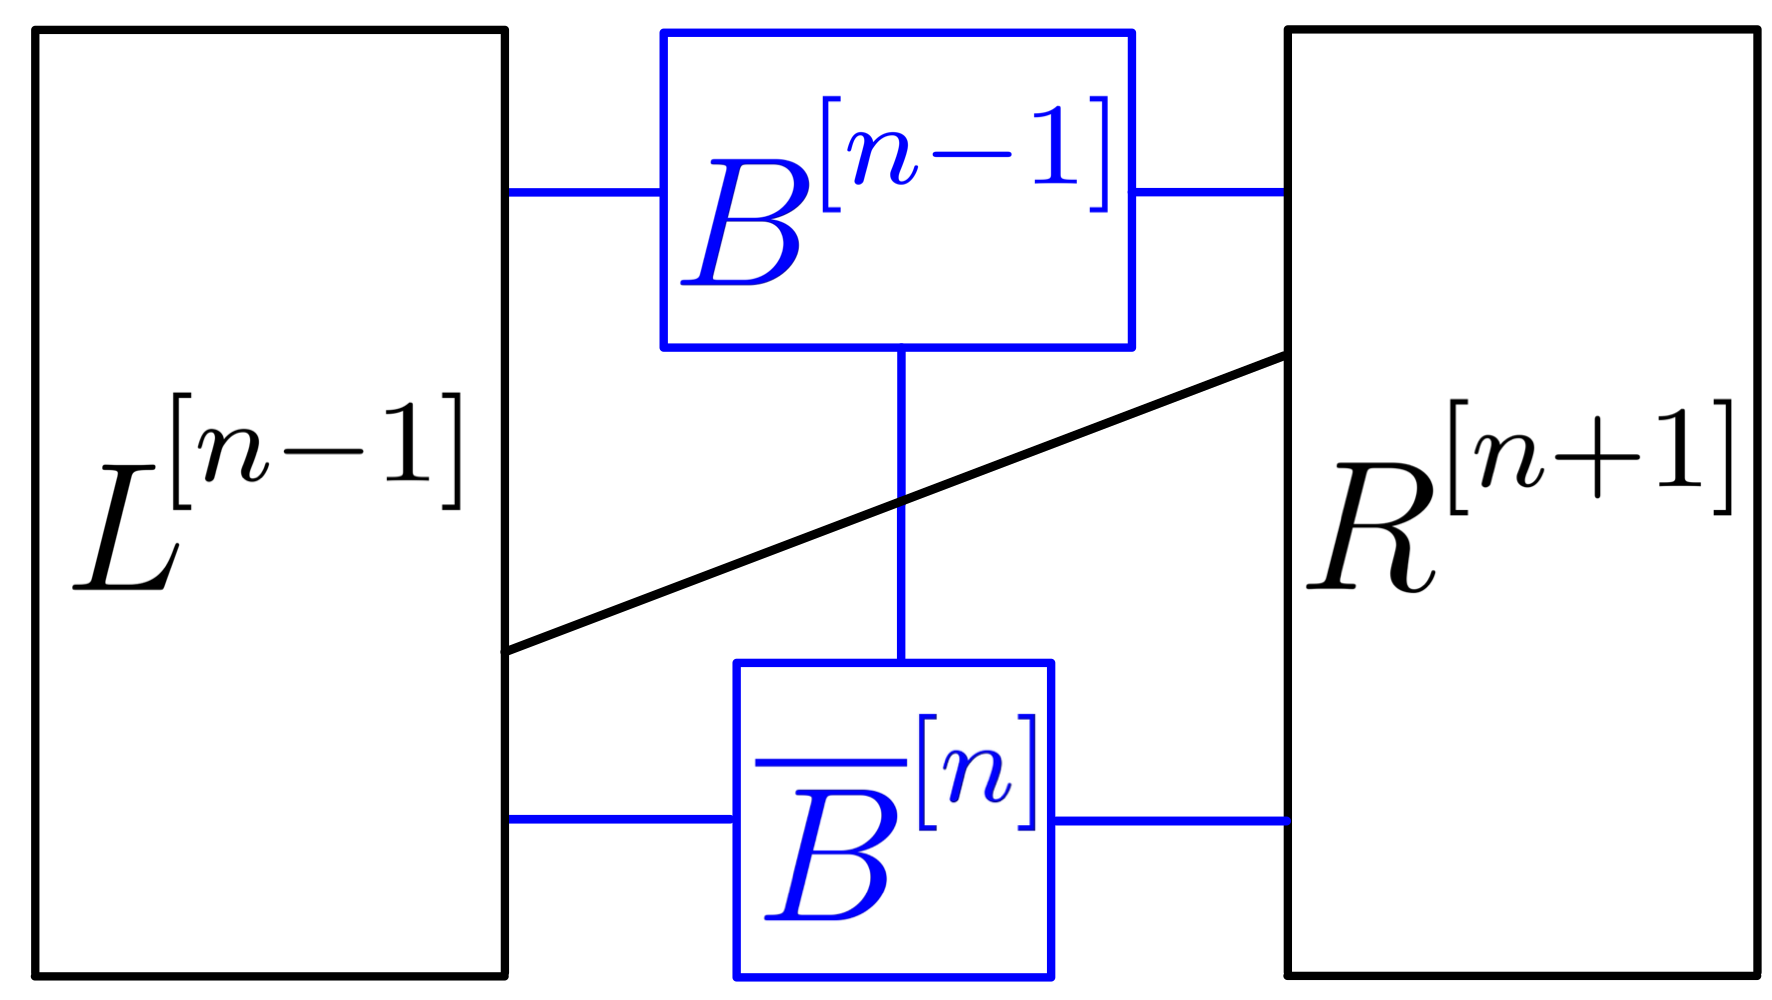
\includegraphics[height=2.cm]{T3.png}} 
	+ 
	\raisebox{-0.45\height}{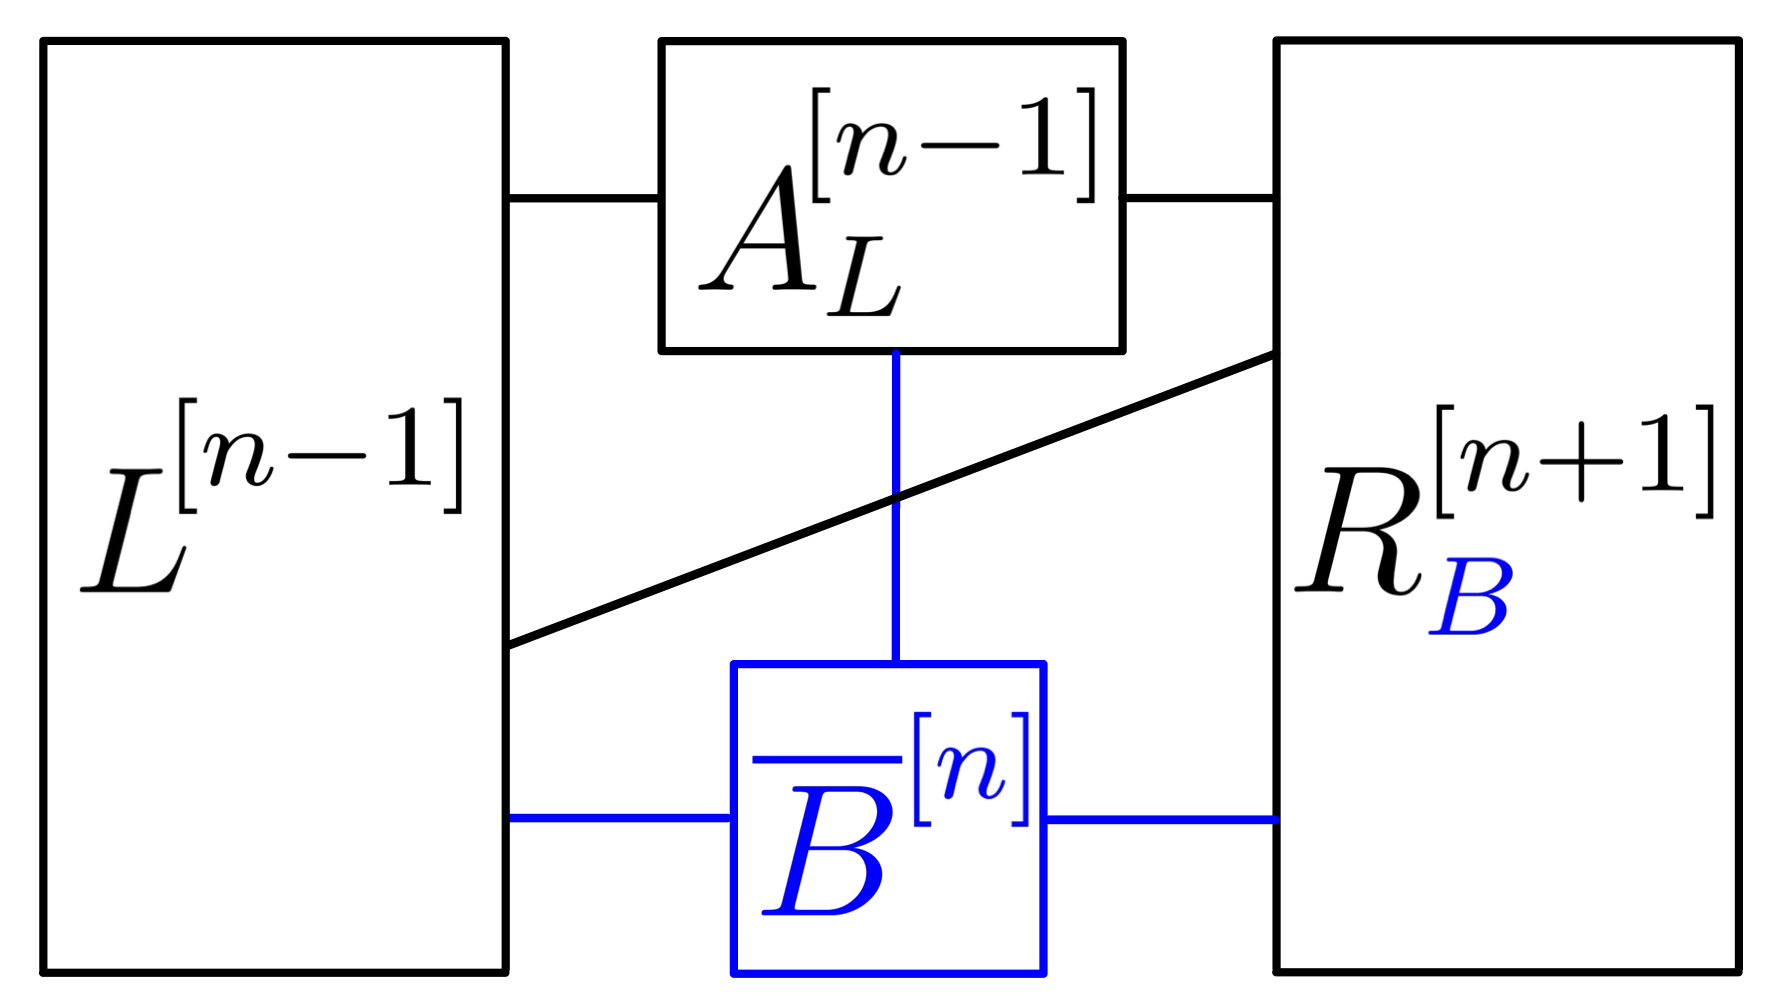
\includegraphics[height=2.cm]{T4.png}} 
	\right]
\end{equation*}

\vspace*{2em}

\begin{equation*}
\begin{array}{l c l}
	\raisebox{-0.5\height}{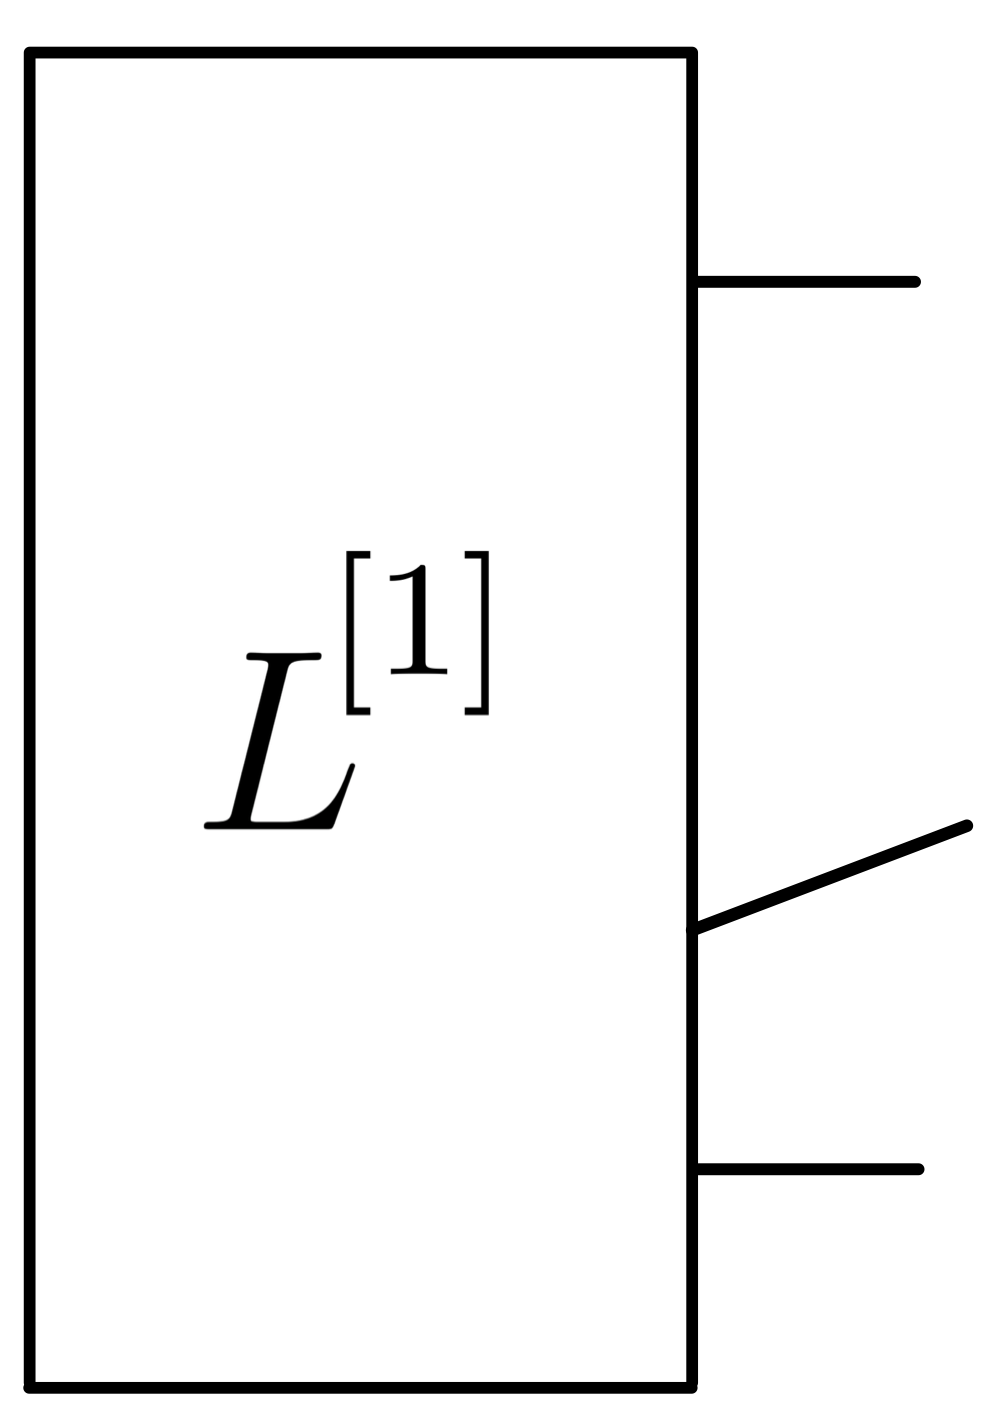
\includegraphics[height=2.cm]{TL1.png}} 
	\:=\:
	\raisebox{-0.5\height}{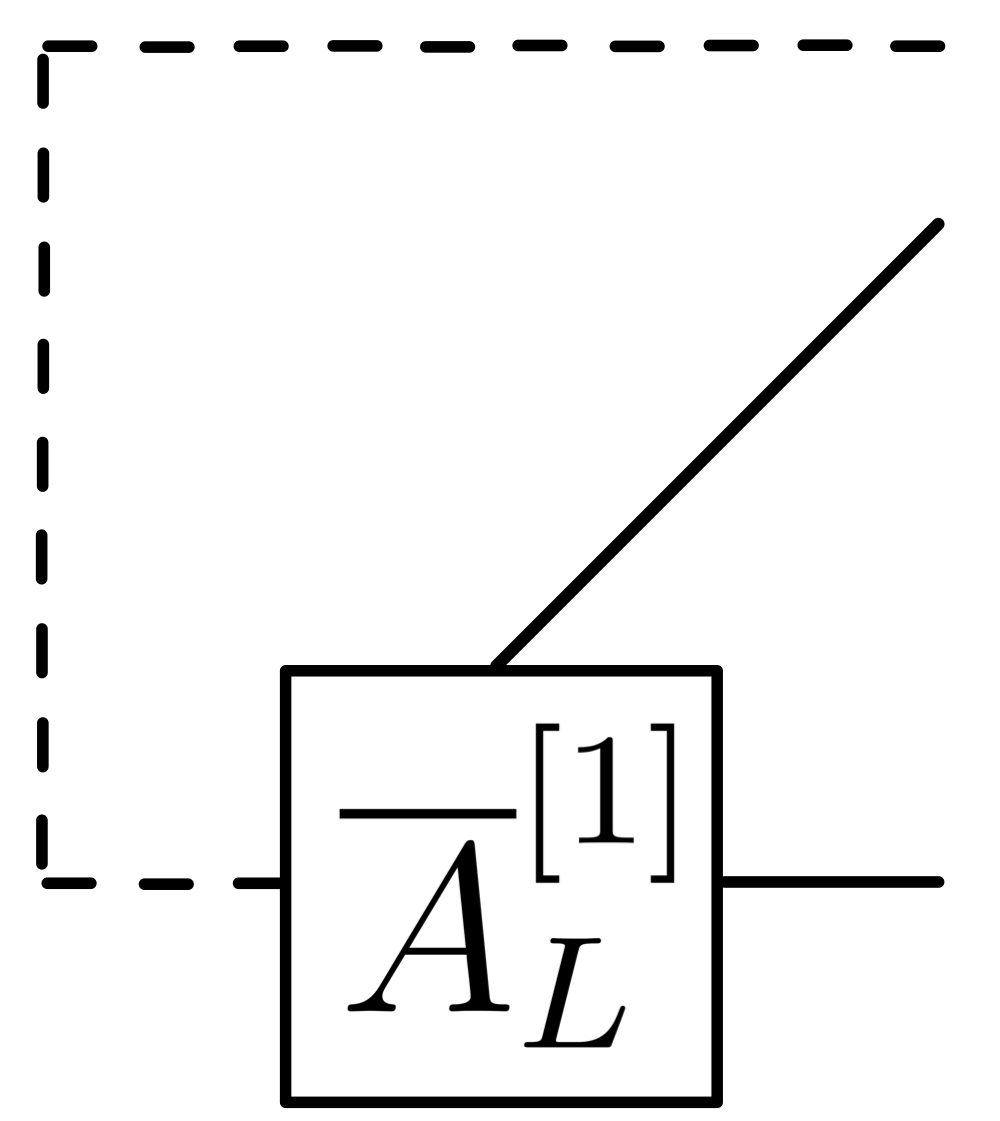
\includegraphics[height=1.6cm]{TL2.png}} 
\hspace{1em}& ; &
	\raisebox{-0.5\height}{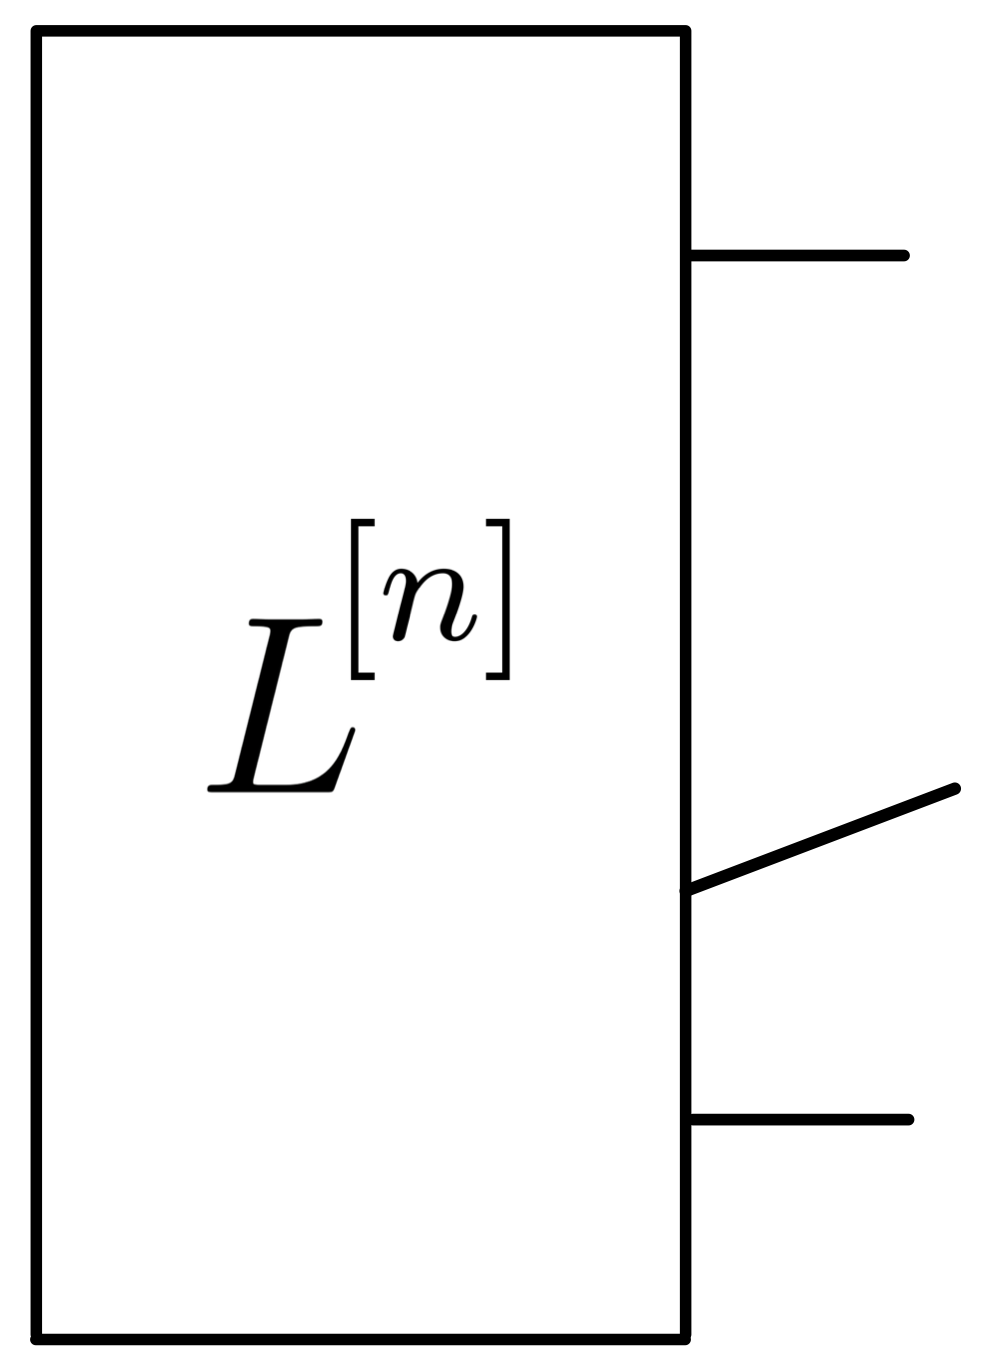
\includegraphics[height=2.cm]{TL3.png}} 
	\:=\:
	\raisebox{-0.5\height}{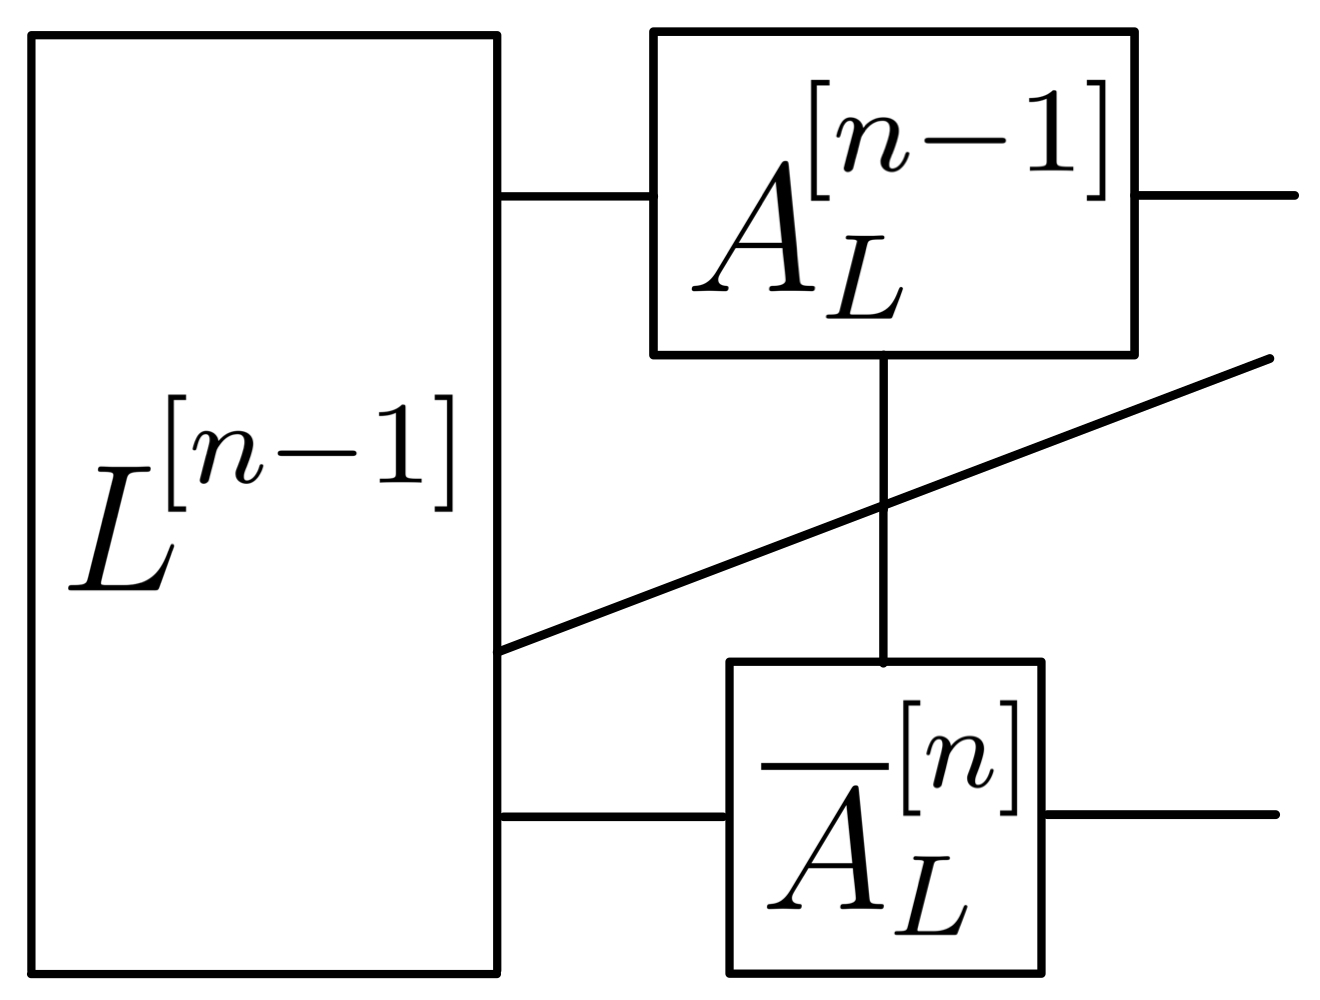
\includegraphics[height=2.cm]{TL4.png}}
	\hspace{1em} \text{\scriptsize{$(n = 2, \ldots, N-1)$}}
\\[3em]
	\raisebox{-0.5\height}{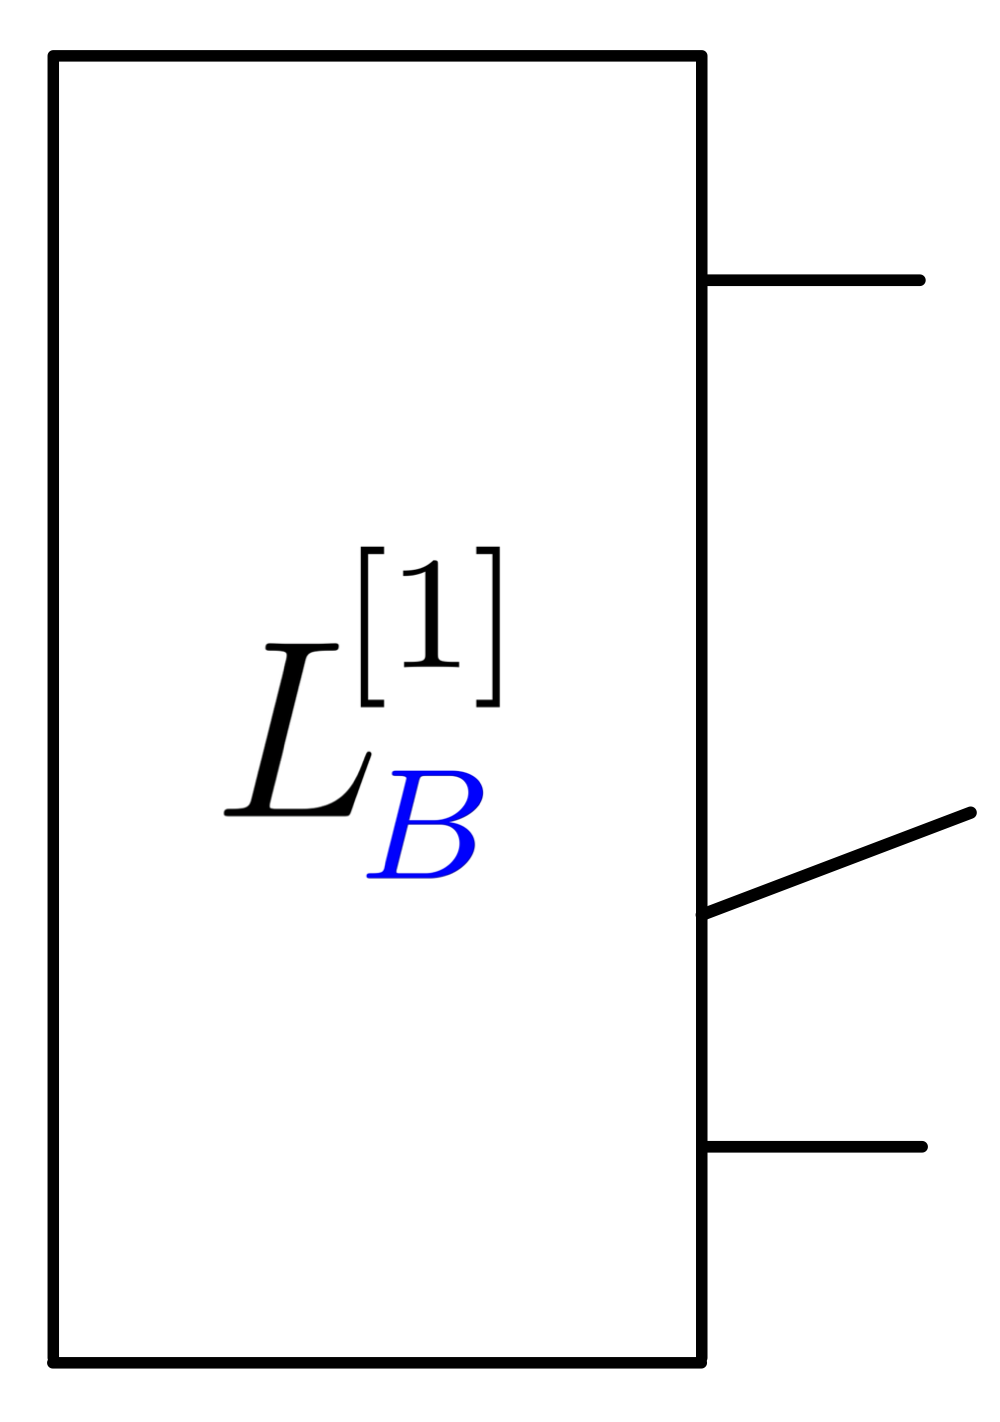
\includegraphics[height=2.cm]{TLB1.png}} 
	\:=\: 0
& ; &
	\raisebox{-0.5\height}{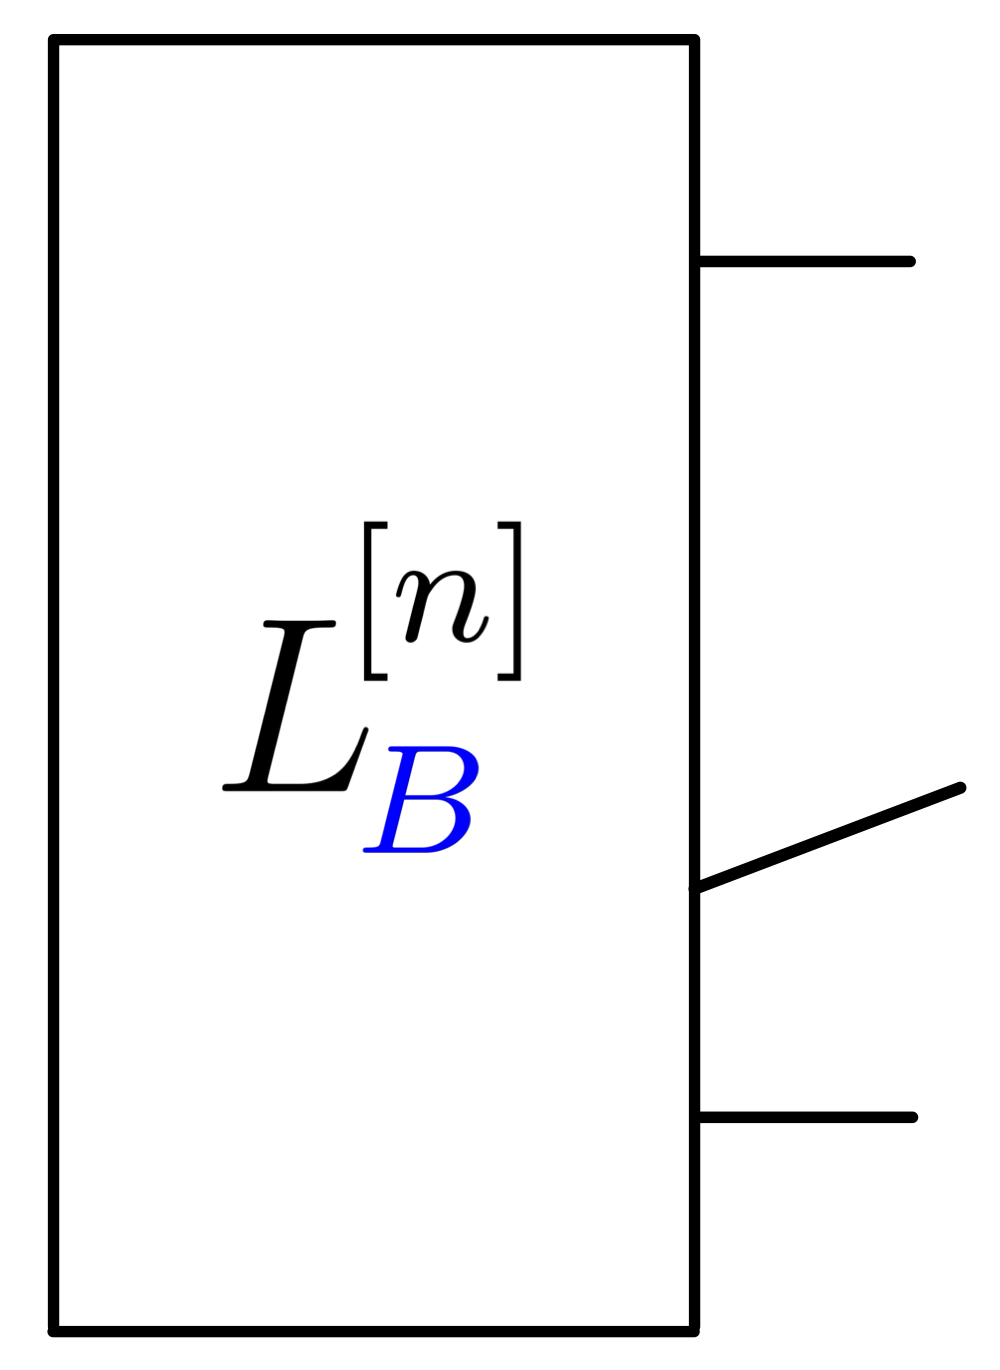
\includegraphics[height=2.cm]{TLB2.png}} 
	\:=\: 
	\raisebox{-0.5\height}{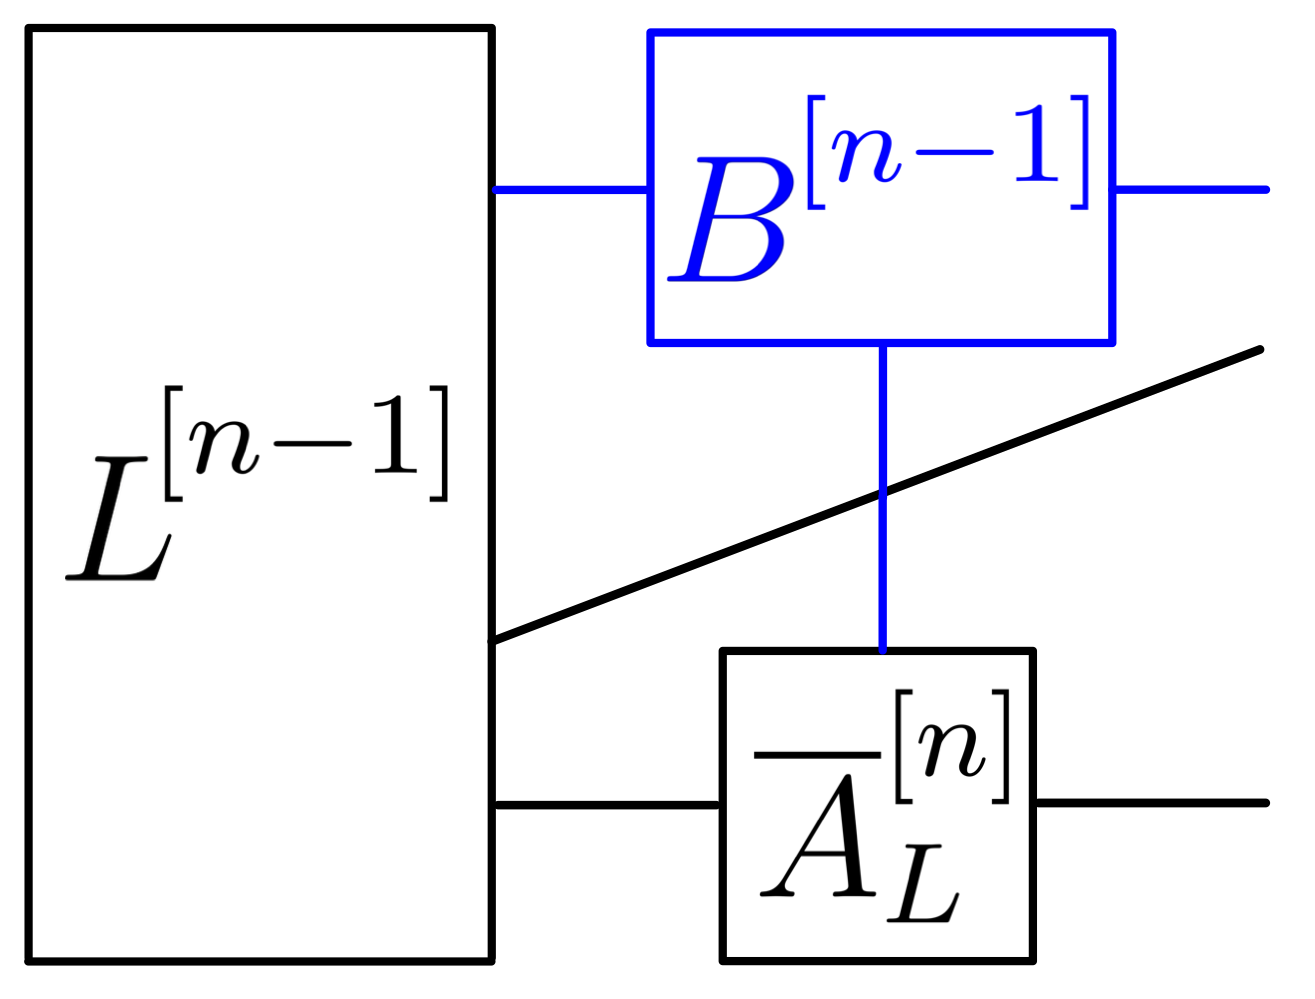
\includegraphics[height=2.cm]{TLB3.png}}
	\:+\:
	\raisebox{-0.5\height}{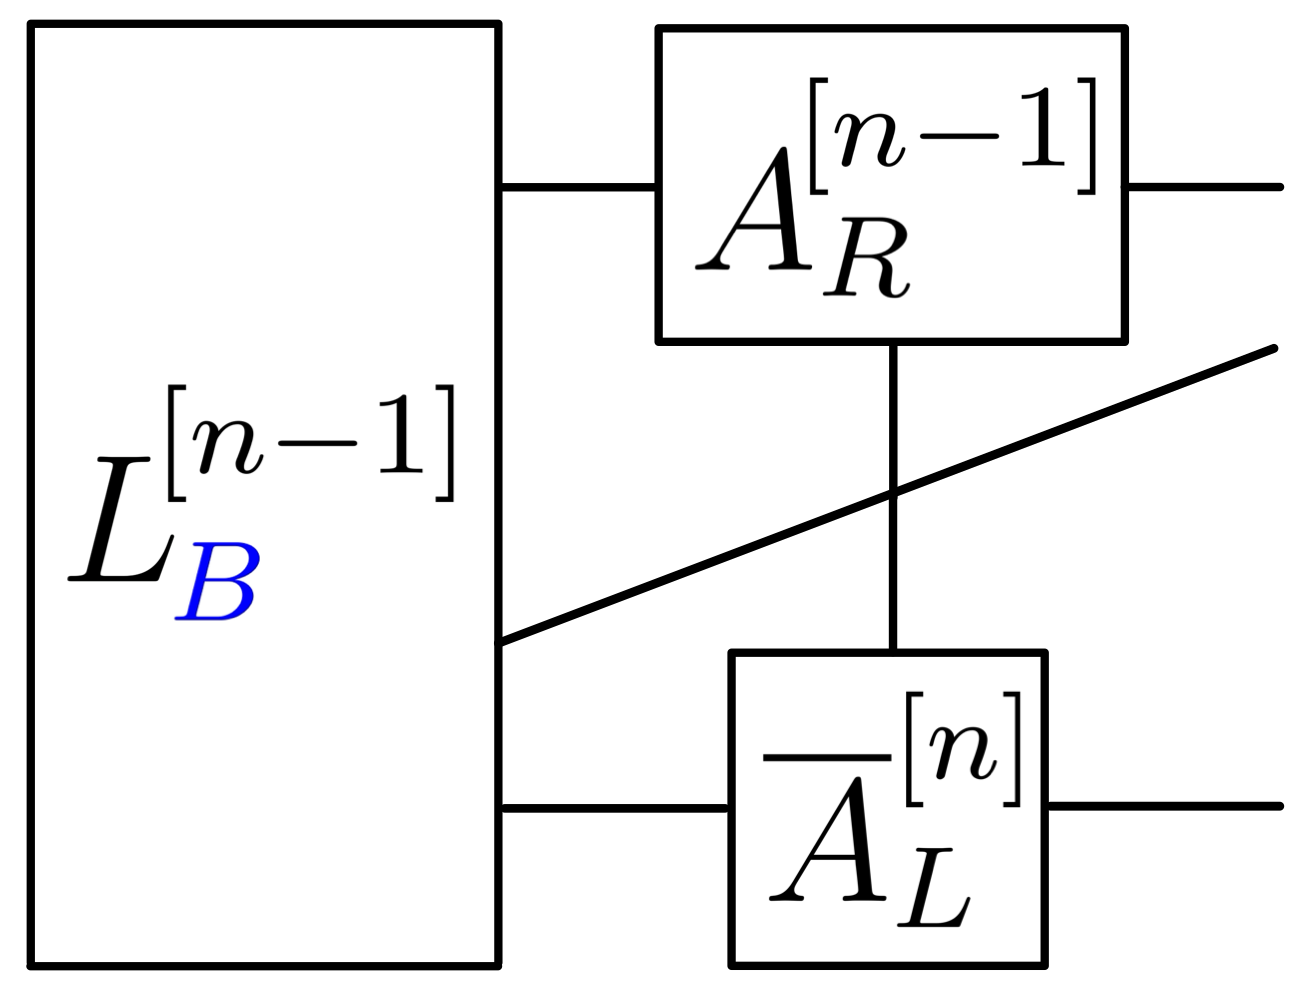
\includegraphics[height=2.cm]{TLB4.png}}
	\hspace{1em} \text{\scriptsize{$(n = 2, \ldots, N-1)$}}
\\[3em]
	\raisebox{-0.5\height}{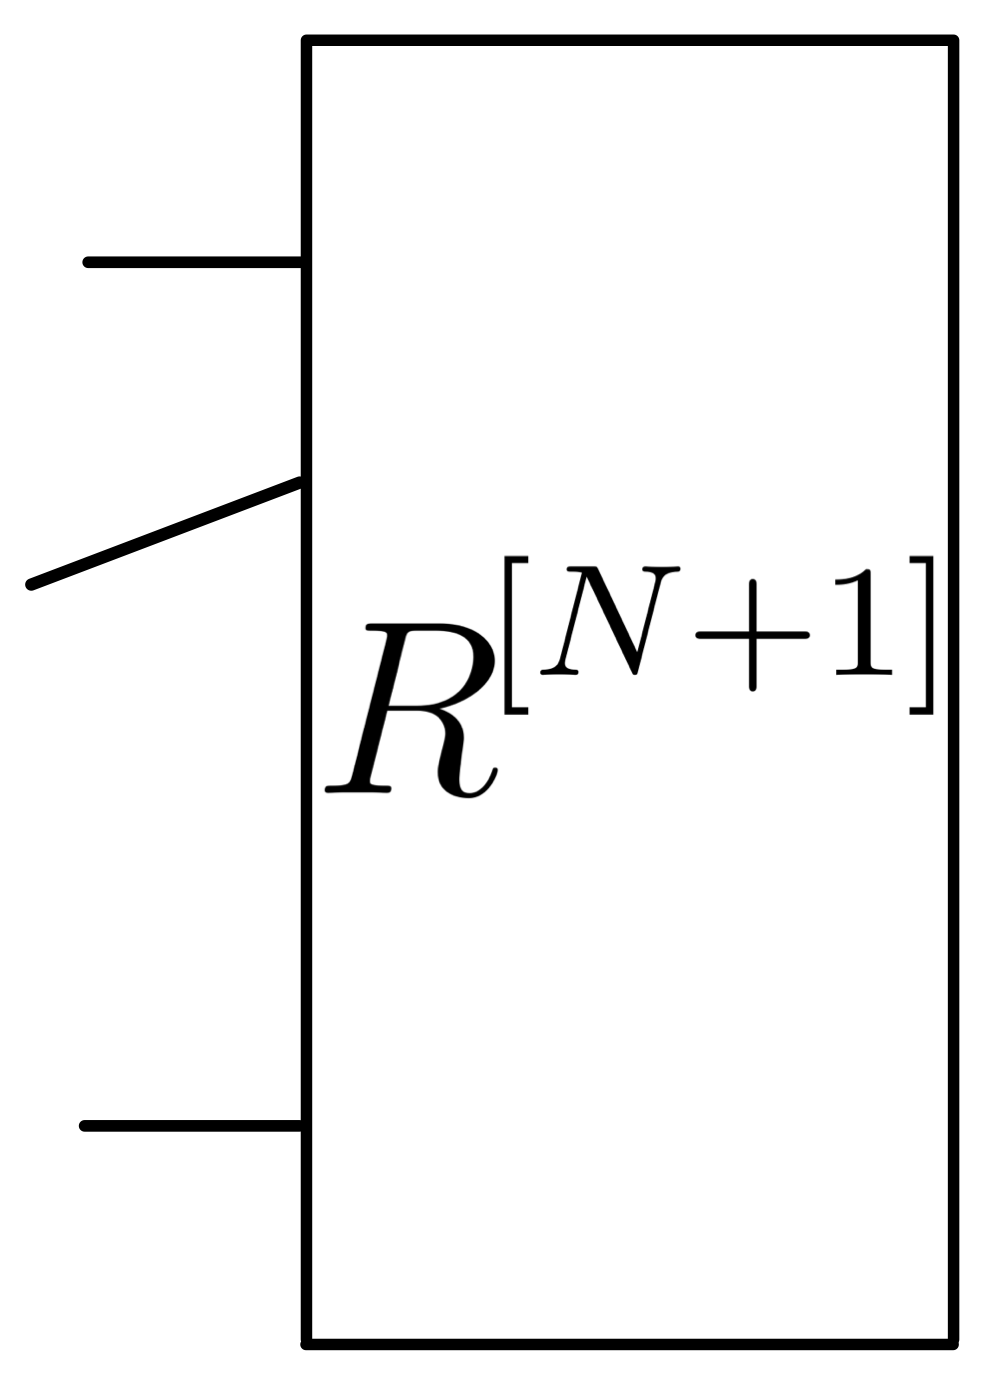
\includegraphics[height=2.cm]{TR1.png}} 
	\:=\:
	\raisebox{-0.5\height}{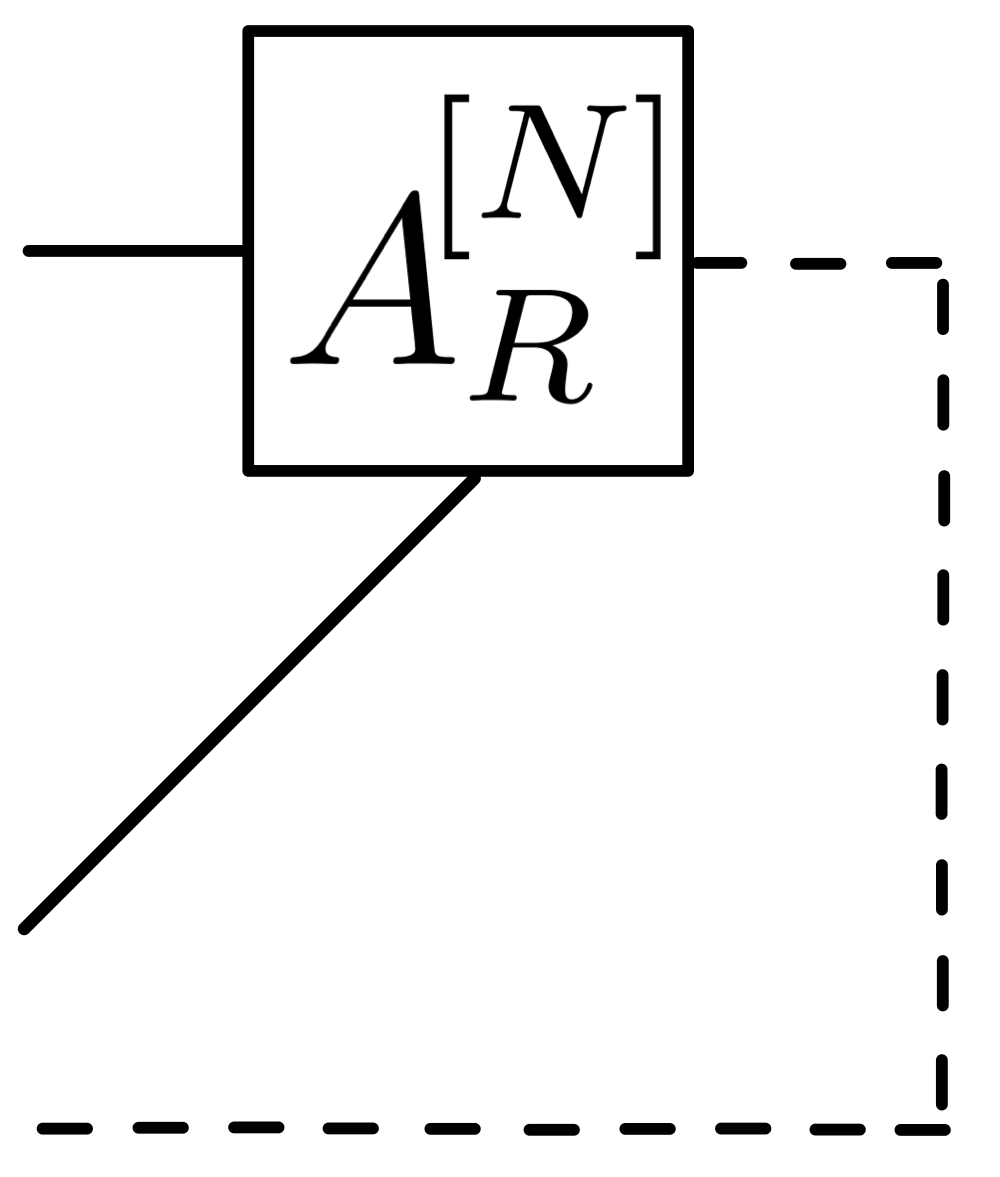
\includegraphics[height=1.6cm]{TR2.png}} 
& ; &
	\raisebox{-0.5\height}{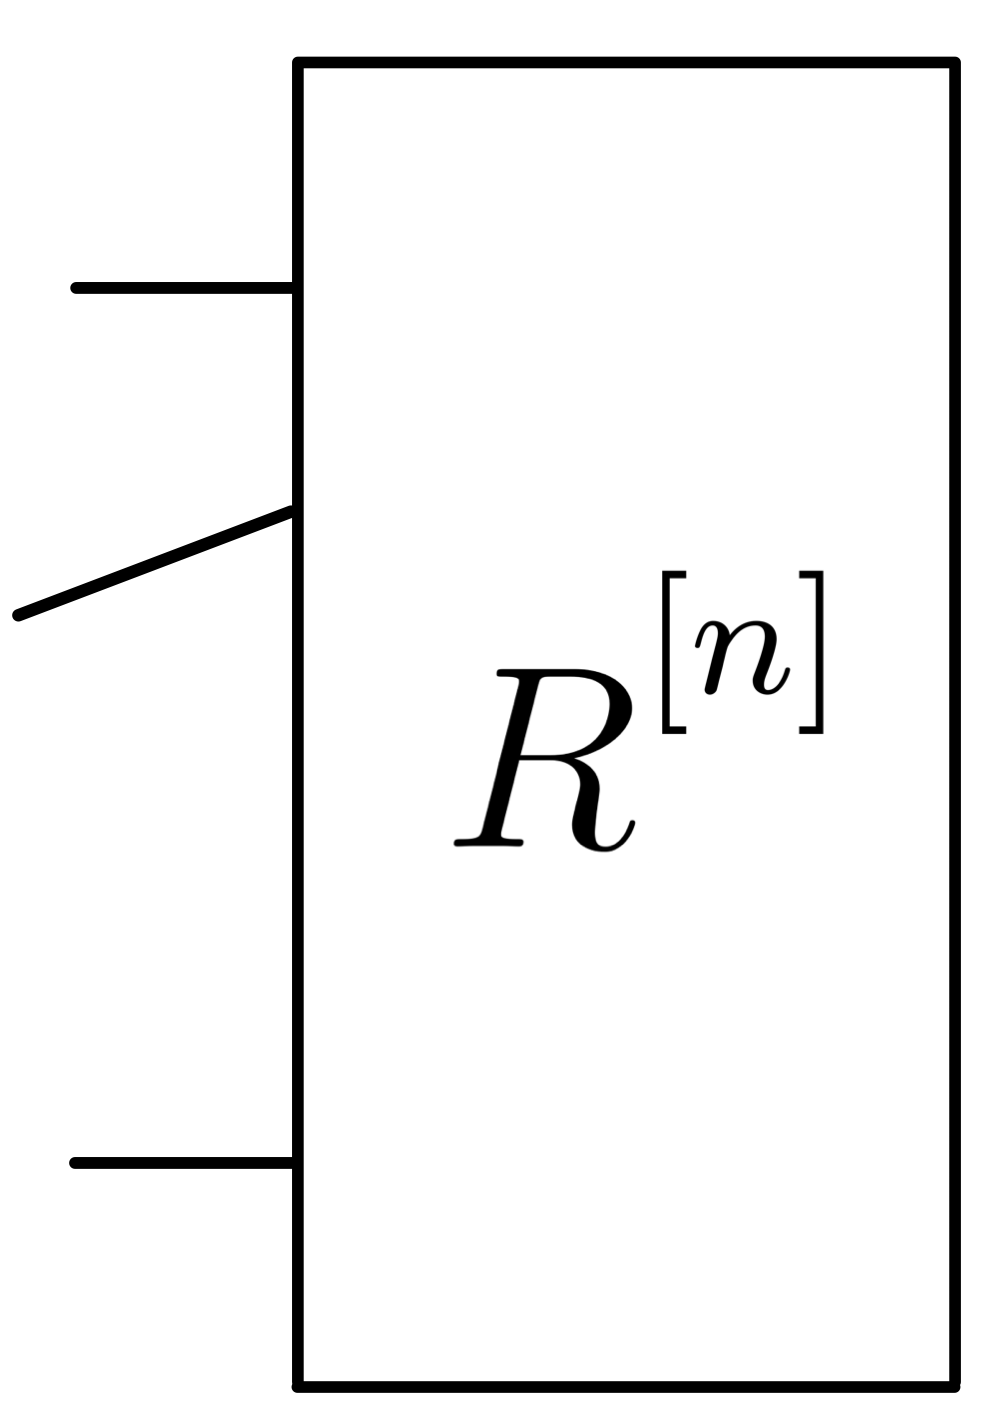
\includegraphics[height=2.cm]{TR3.png}} 
	\:=\: 
	\raisebox{-0.5\height}{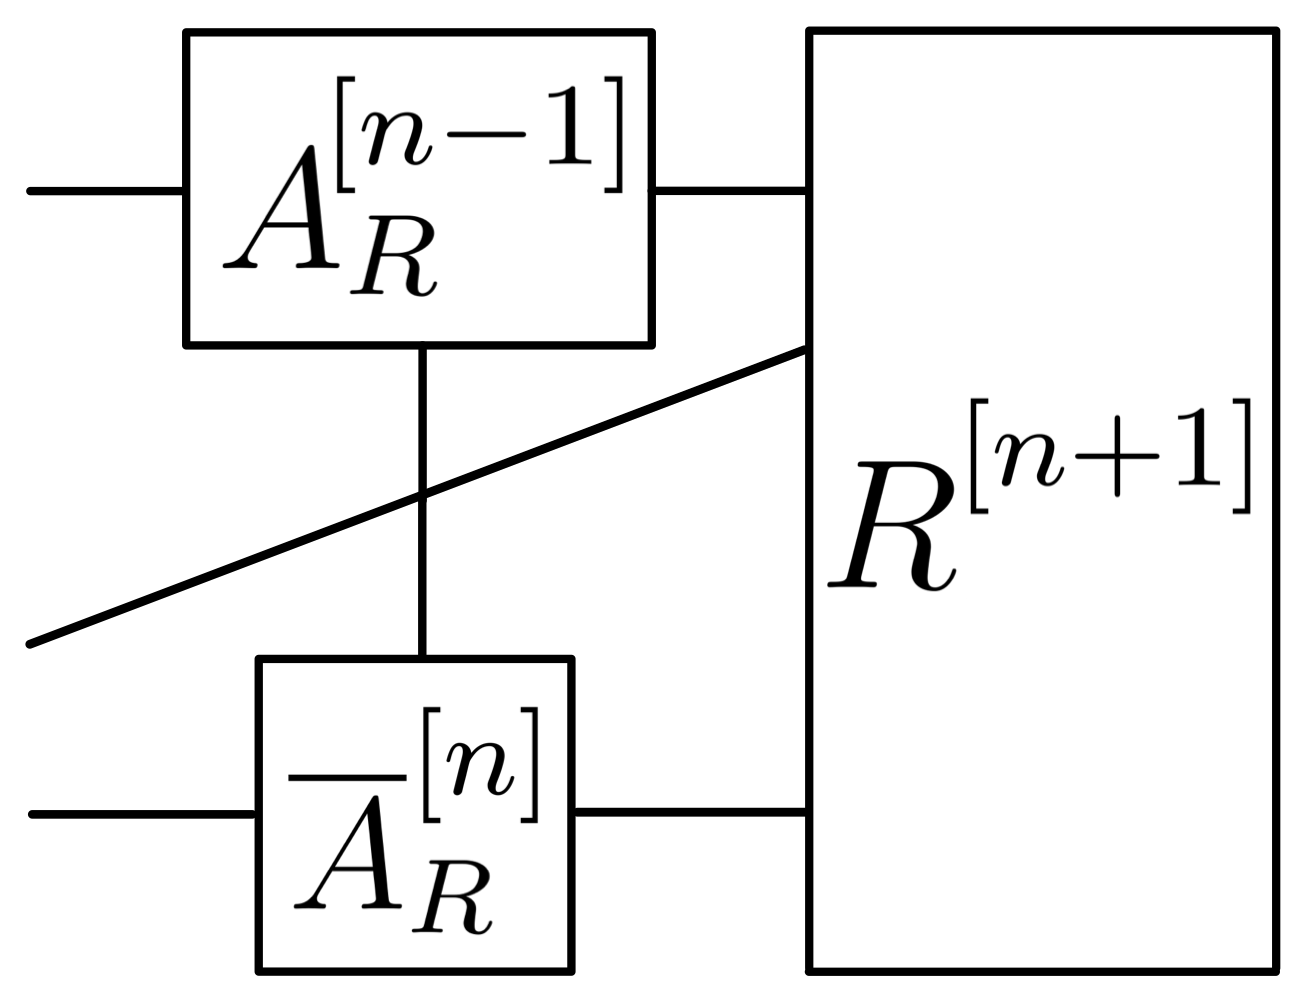
\includegraphics[height=2.cm]{TR4.png}}
	\hspace{1em} \text{\scriptsize{$(n = N, \ldots, 2)$}}
\\[3em]
	\raisebox{-0.5\height}{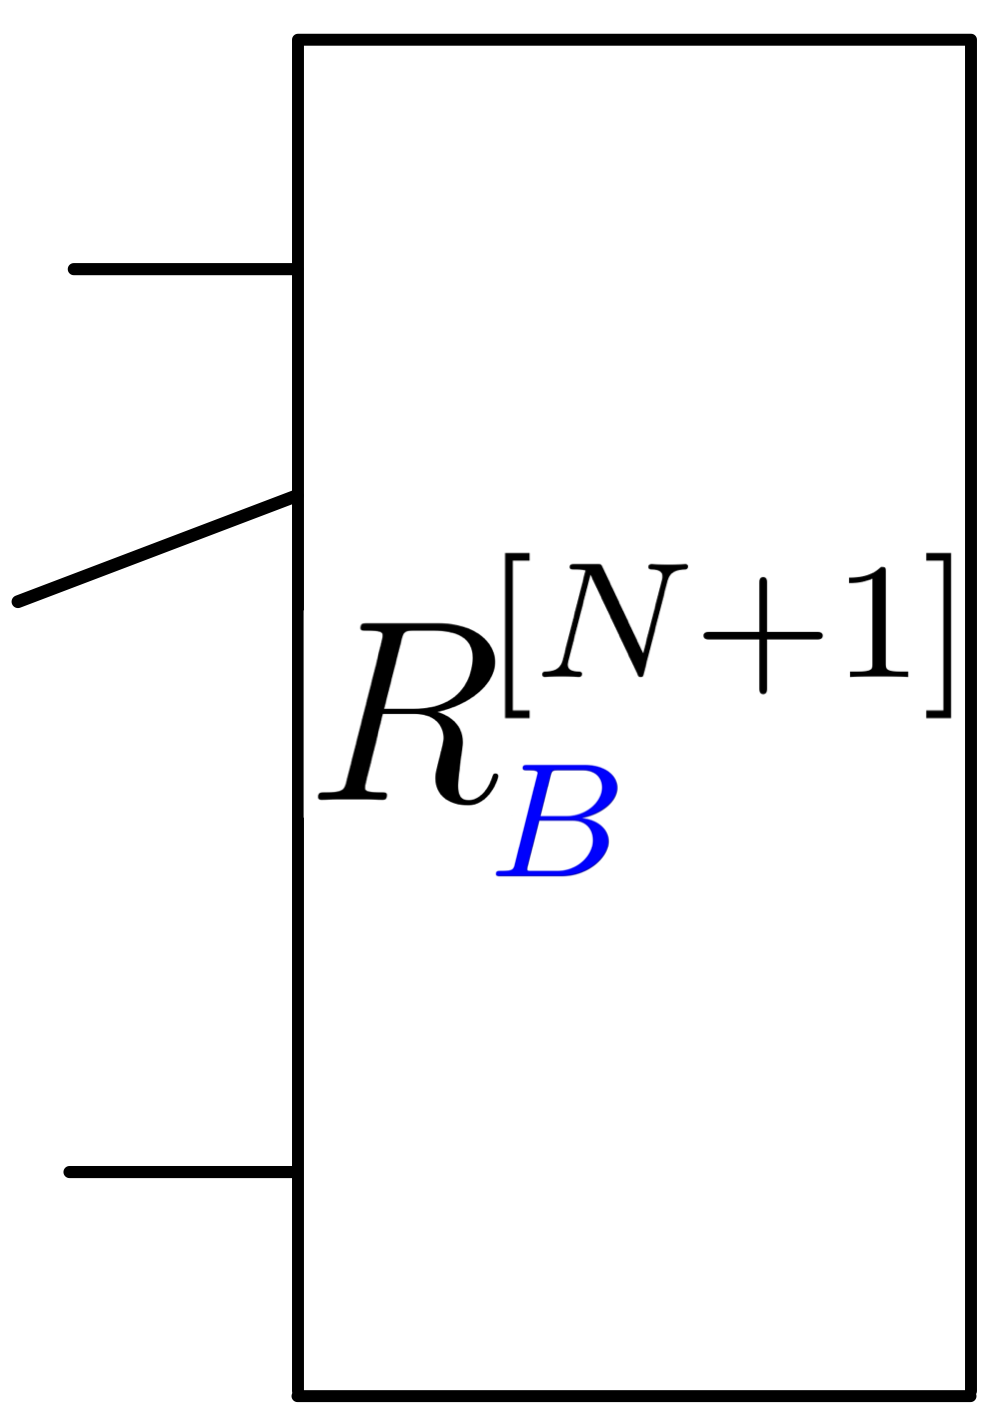
\includegraphics[height=2.cm]{TRB1.png}} 
	\:=\:
	\raisebox{-0.5\height}{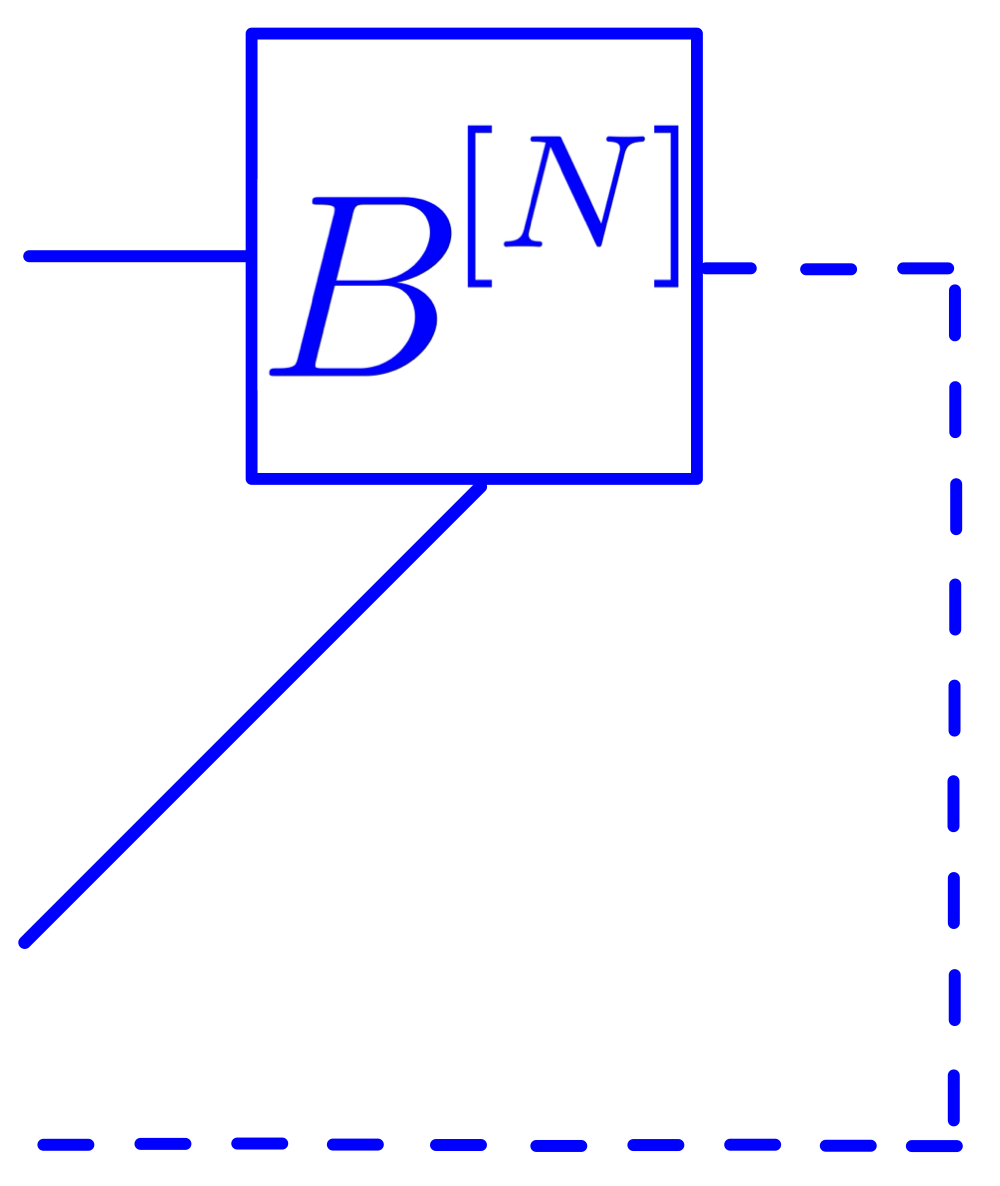
\includegraphics[height=1.6cm]{TRB2.png}} 
& ; &
	\raisebox{-0.5\height}{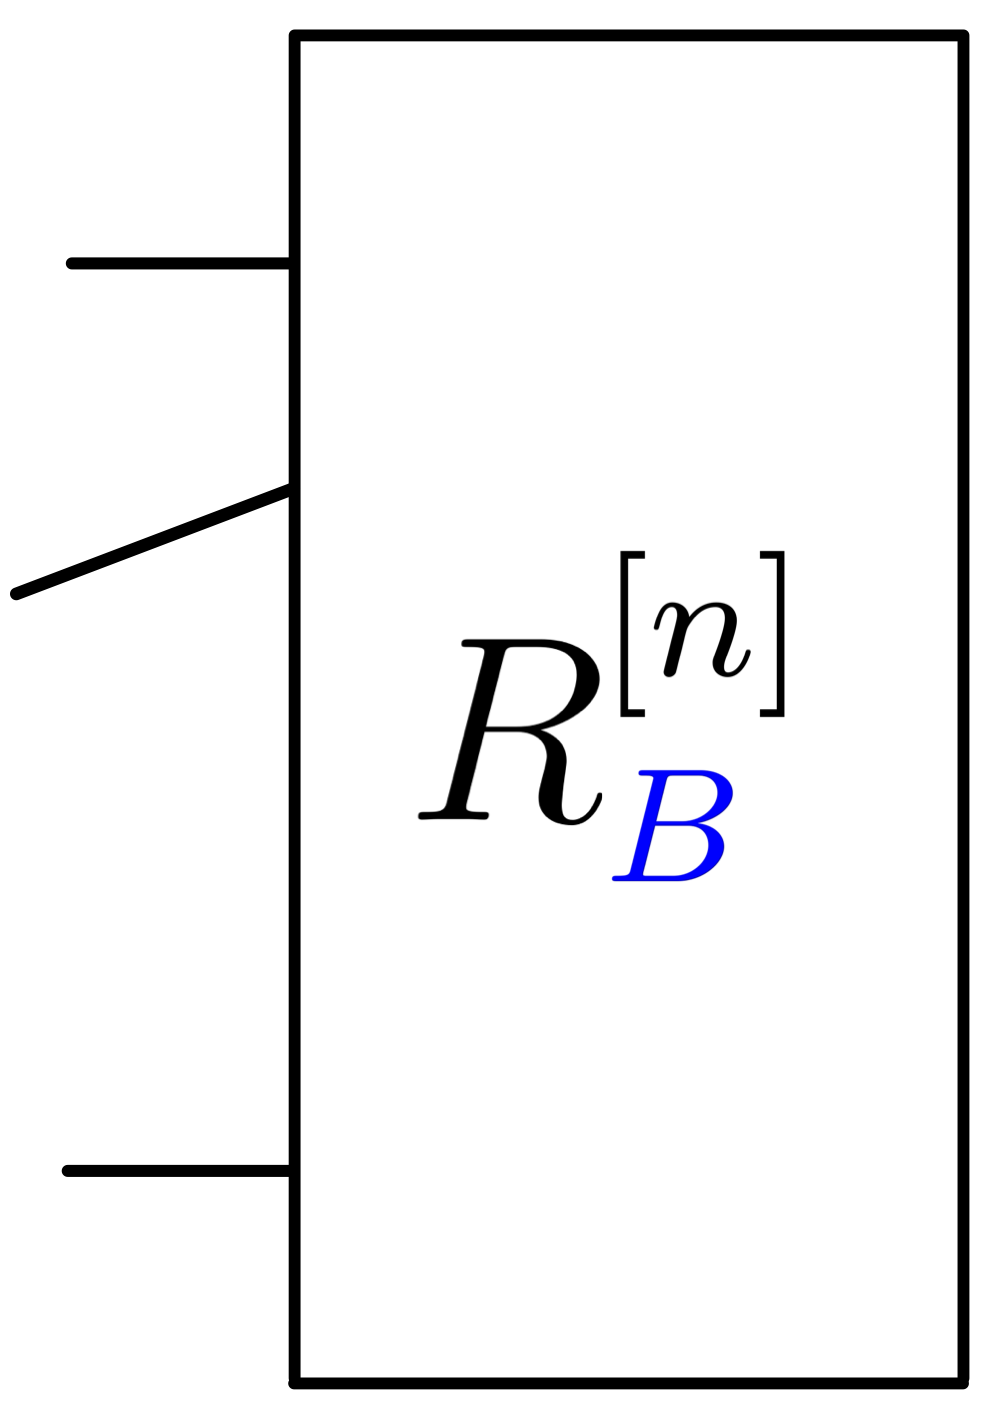
\includegraphics[height=2.cm]{TRB3.png}} 
	\:=\: 
	\raisebox{-0.5\height}{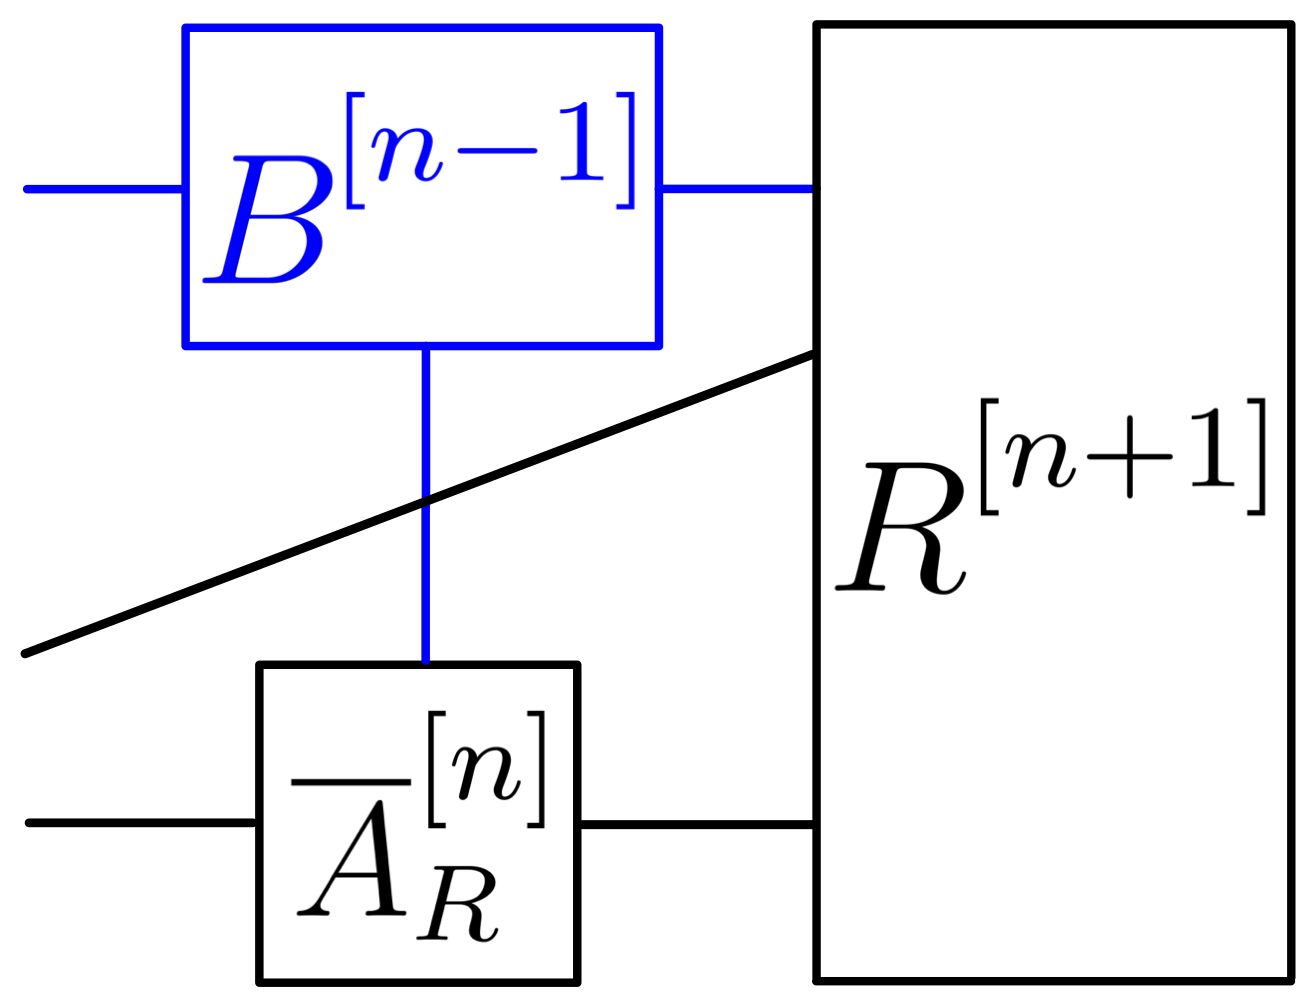
\includegraphics[height=2.cm]{TRB4.png}}
	\:+\:
	\raisebox{-0.5\height}{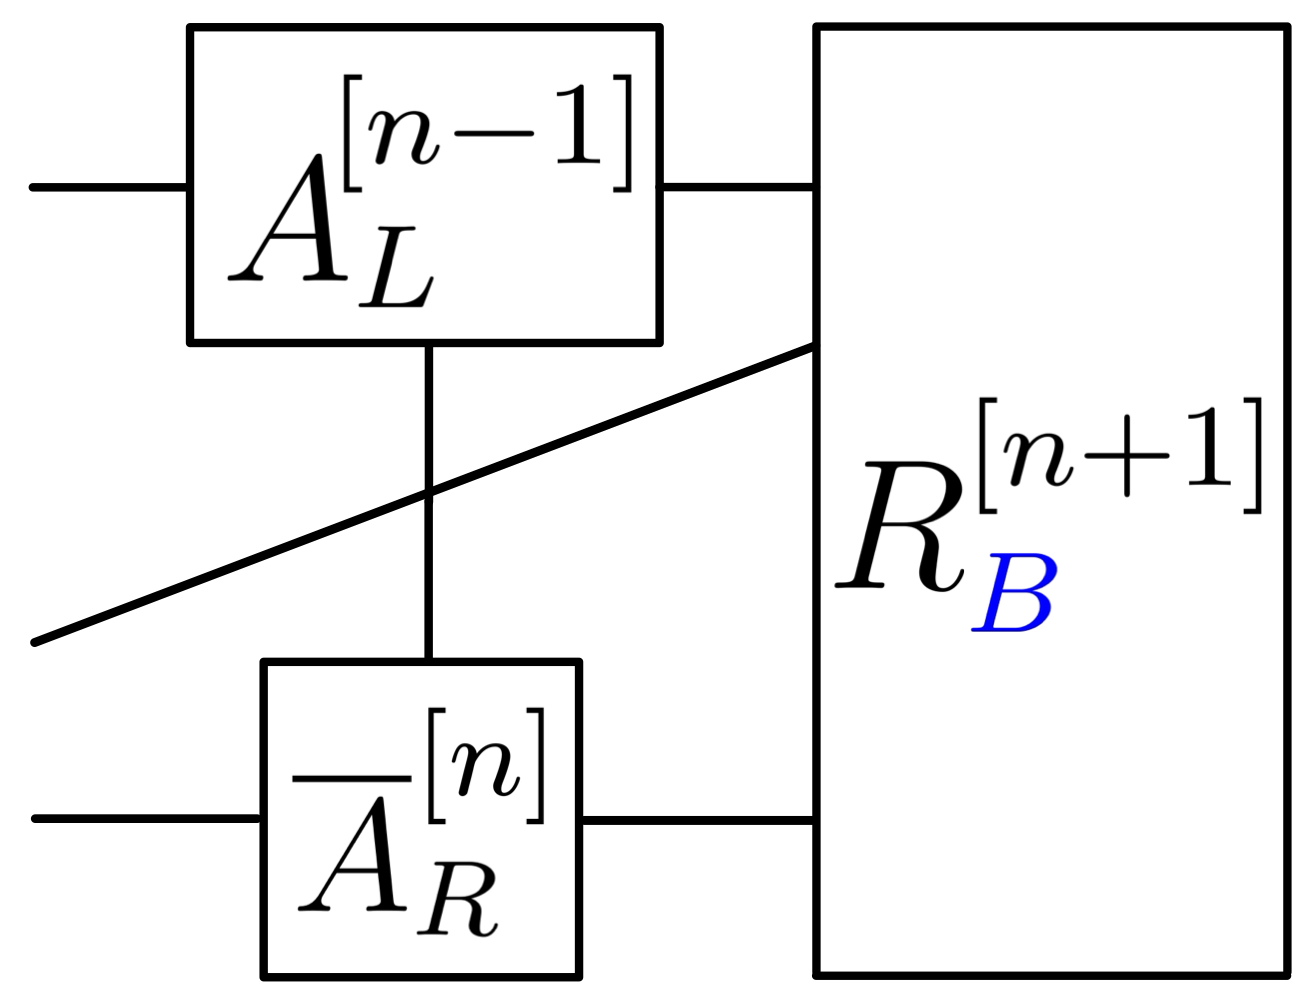
\includegraphics[height=2.cm]{TRB5.png}}
	\hspace{1em} \text{\scriptsize{$(n = N, \ldots, 2)$}}
\end{array}
\end{equation*}

\newpage
% Teff_dagger
\begin{align*}
\begin{split}
	\textcolor{blue}{\tbra{\overline{B}}} &T_{\text{eff}}^{\dagger} \textcolor{blue}{\tket{B}} \\
	&=
\end{split}
\end{align*}
\vspace*{-0.5cm}
\begin{equation*}
	\sum_{n=1}^{N-1} \left[
	\raisebox{-0.45\height}{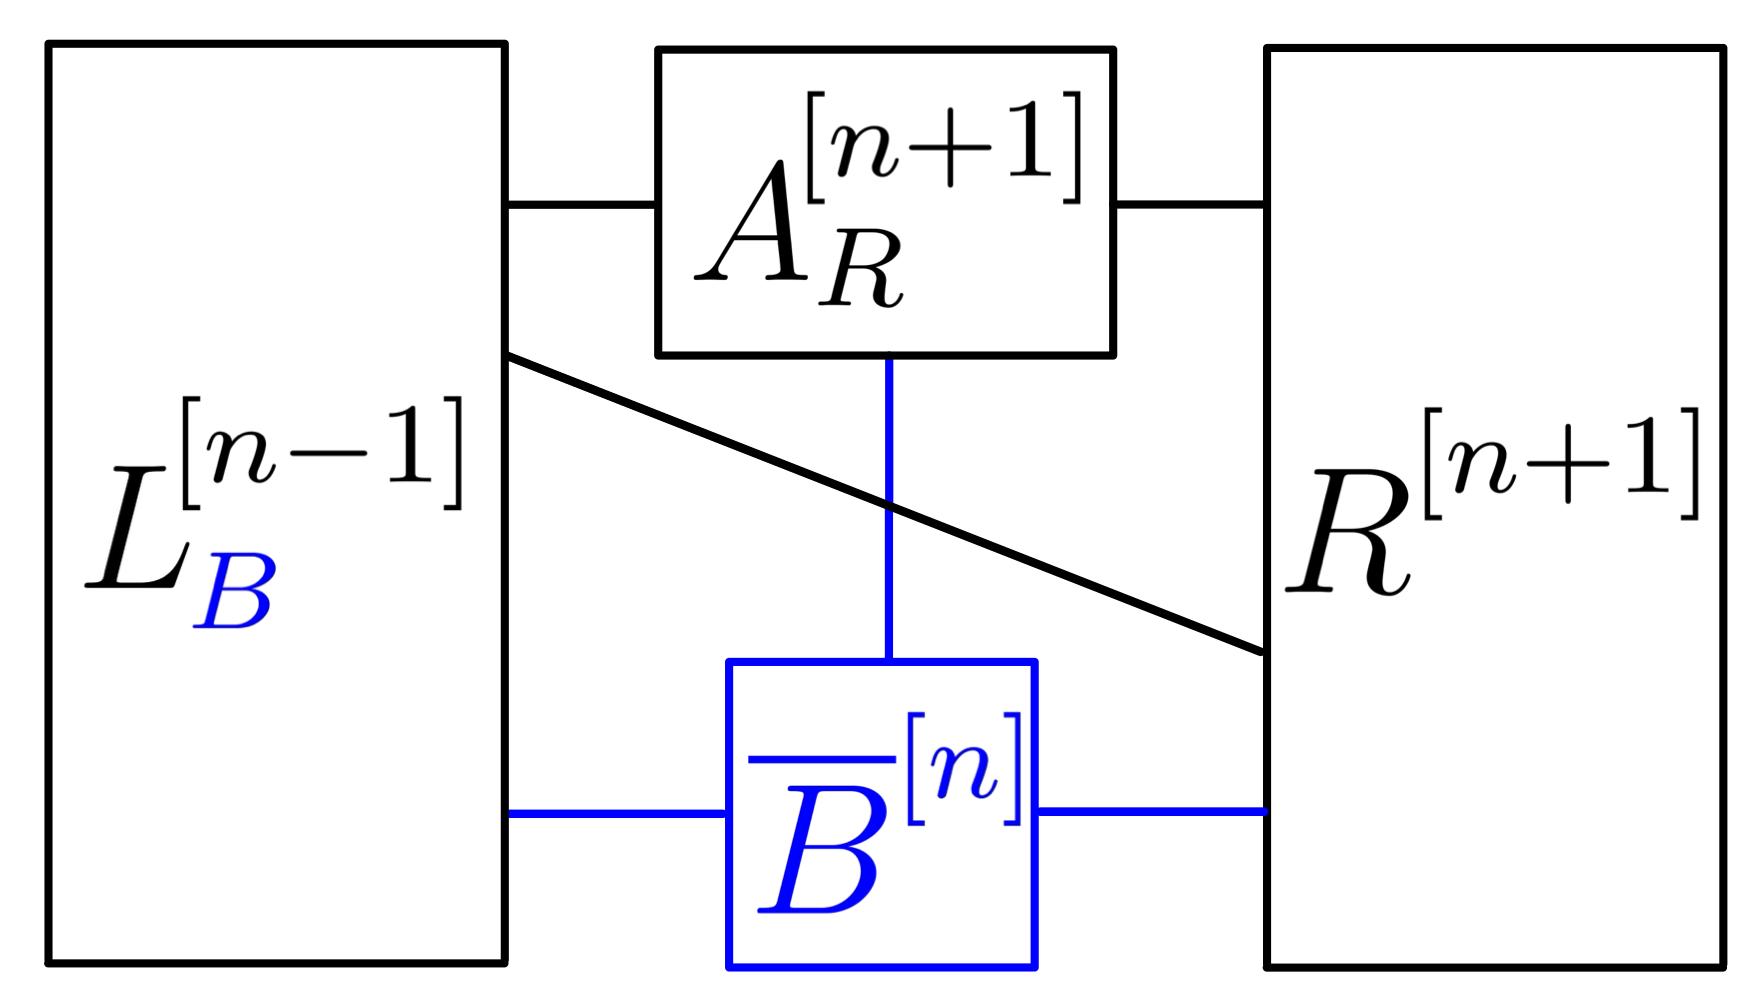
\includegraphics[height=2.cm]{Tdagger1.png}} 
	+
	\raisebox{-0.45\height}{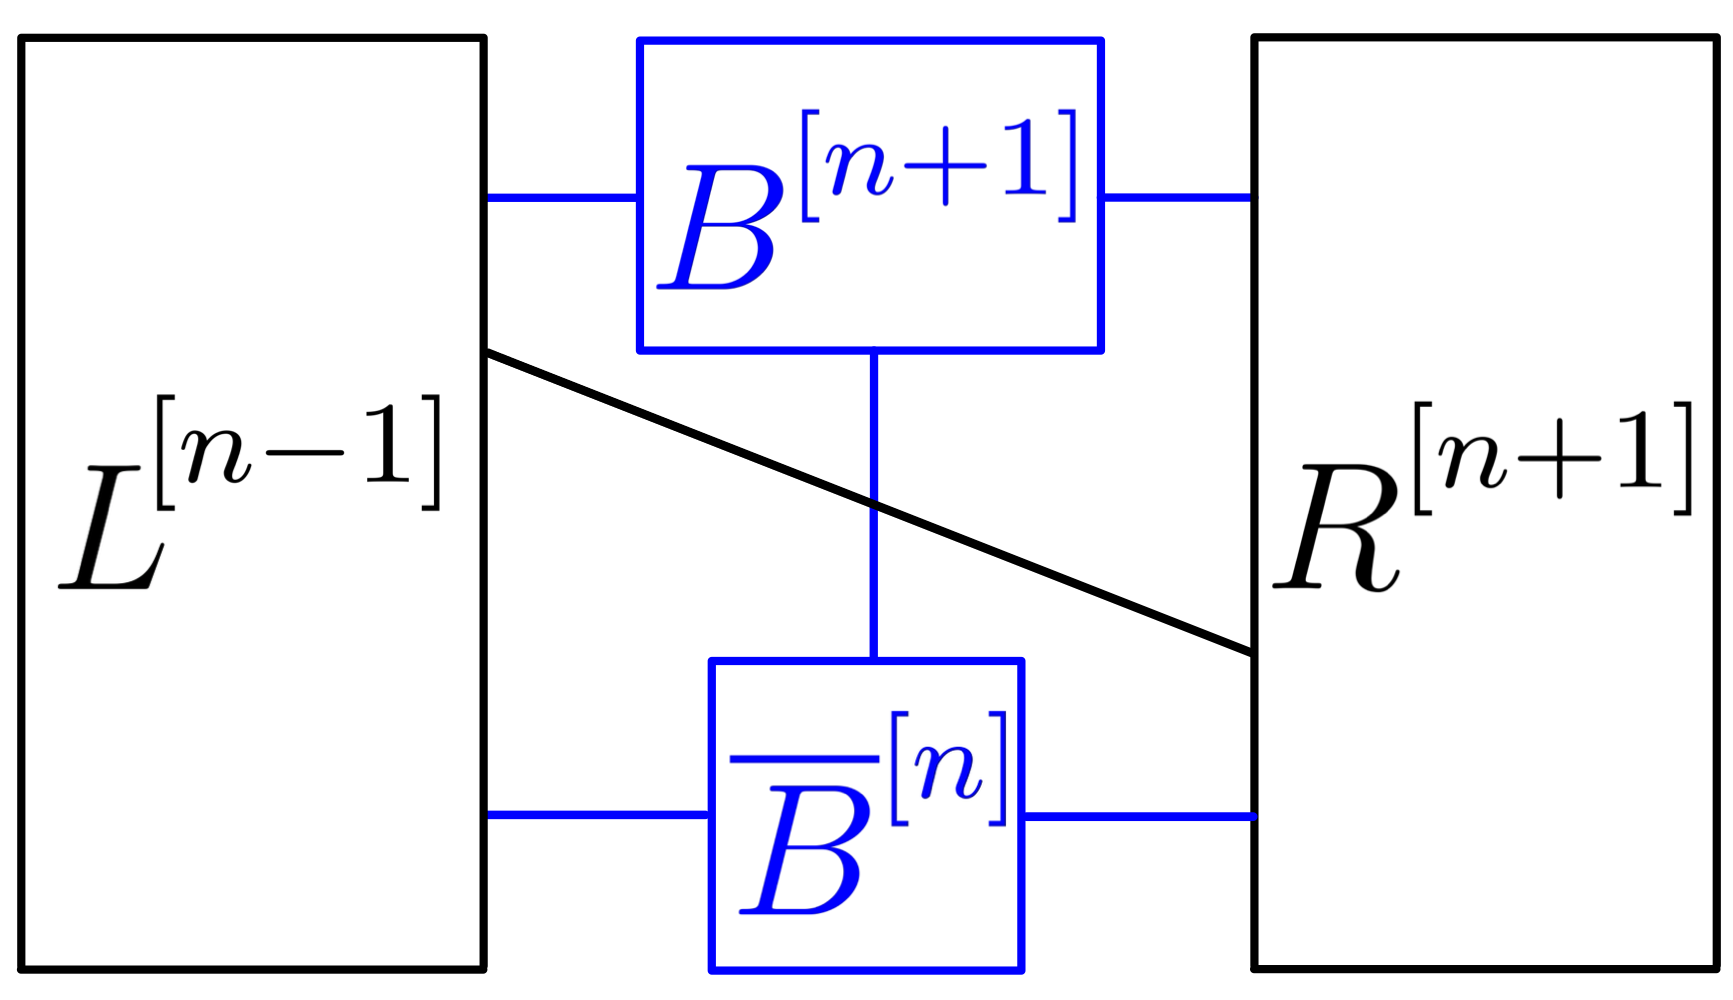
\includegraphics[height=2.cm]{Tdagger2.png}}
	+
	\raisebox{-0.45\height}{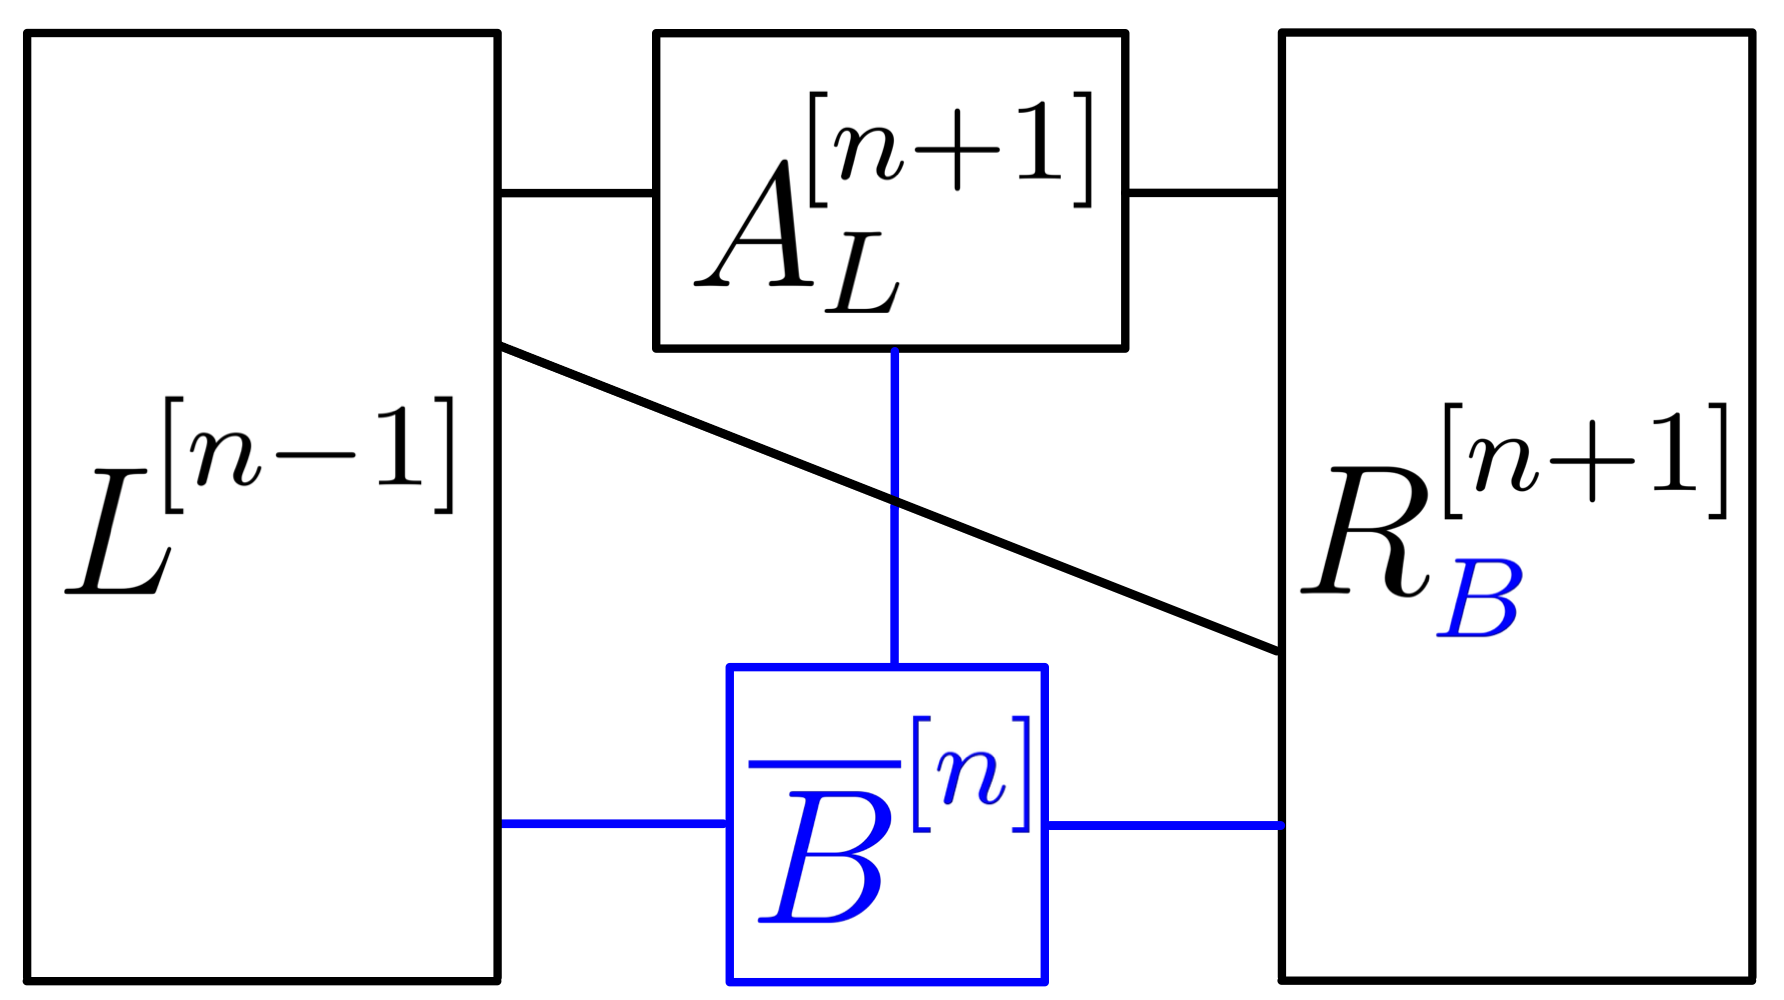
\includegraphics[height=2.cm]{Tdagger3.png}} 
	\right] 
	\:+\:
	\raisebox{-0.45\height}{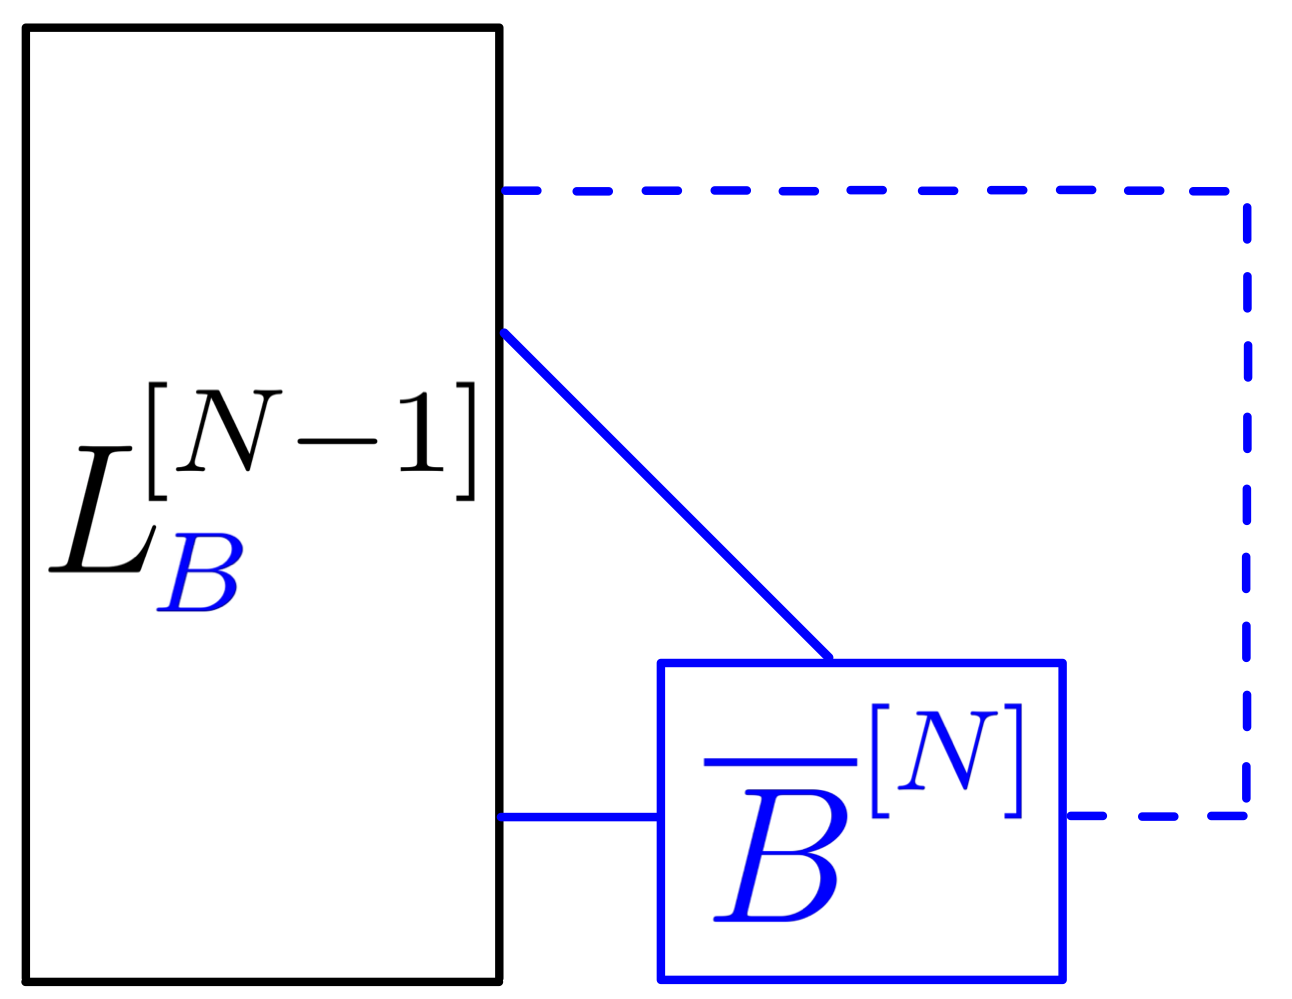
\includegraphics[height=2.cm]{Tdagger4.png}}
\end{equation*}

\vspace*{2em}

\begin{equation*}
\begin{array}{l c l}
	\raisebox{-0.5\height}{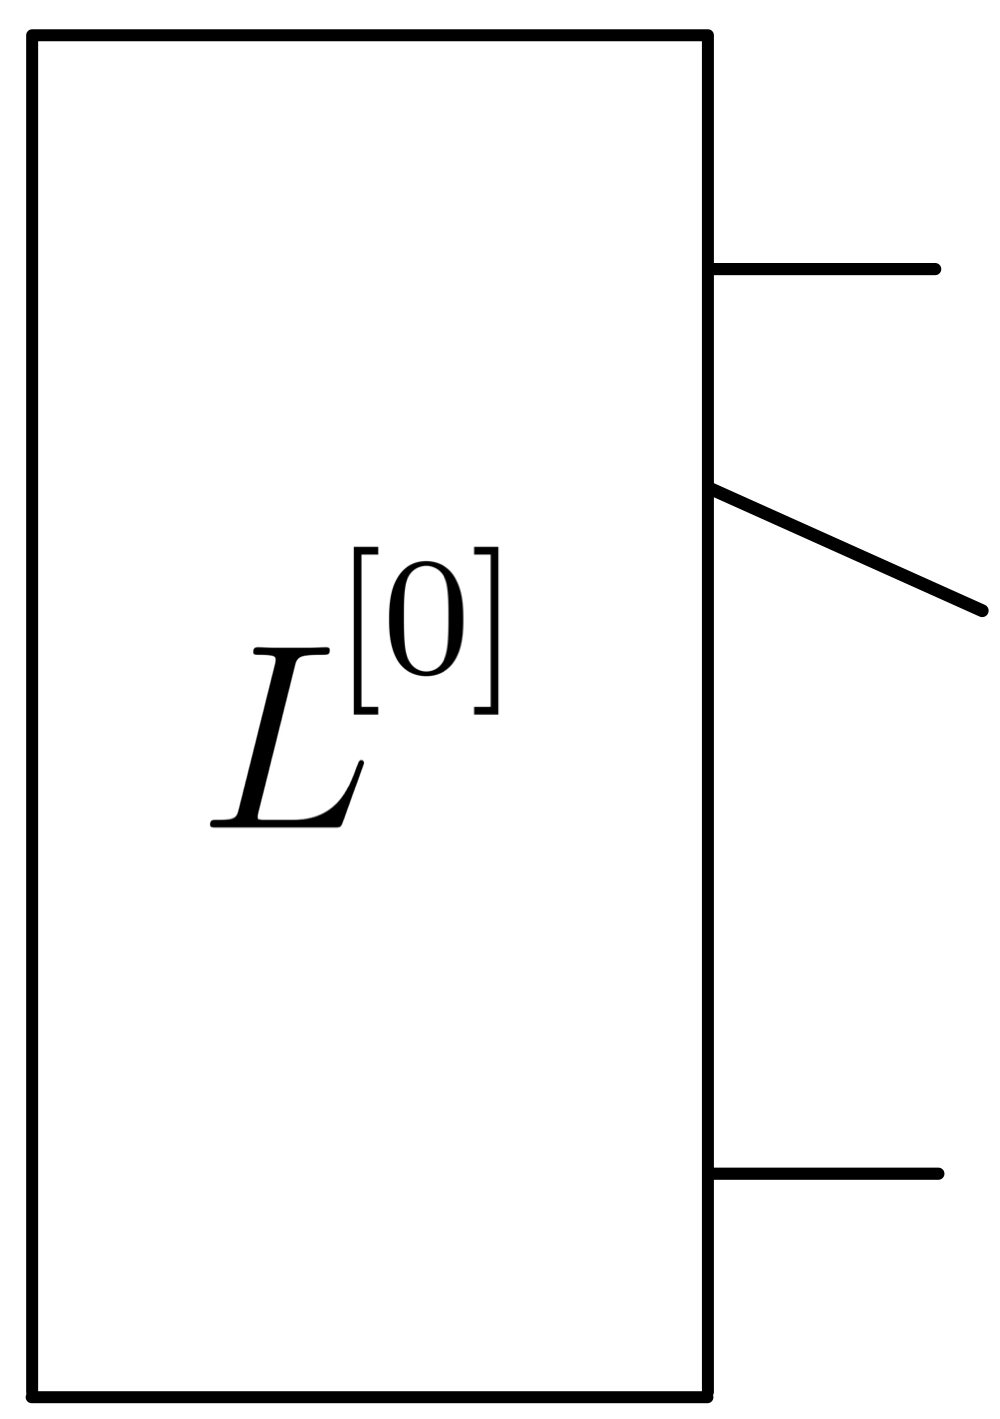
\includegraphics[height=2.cm]{TdaggerL1.png}} 
	\:=\:
	\raisebox{-0.5\height}{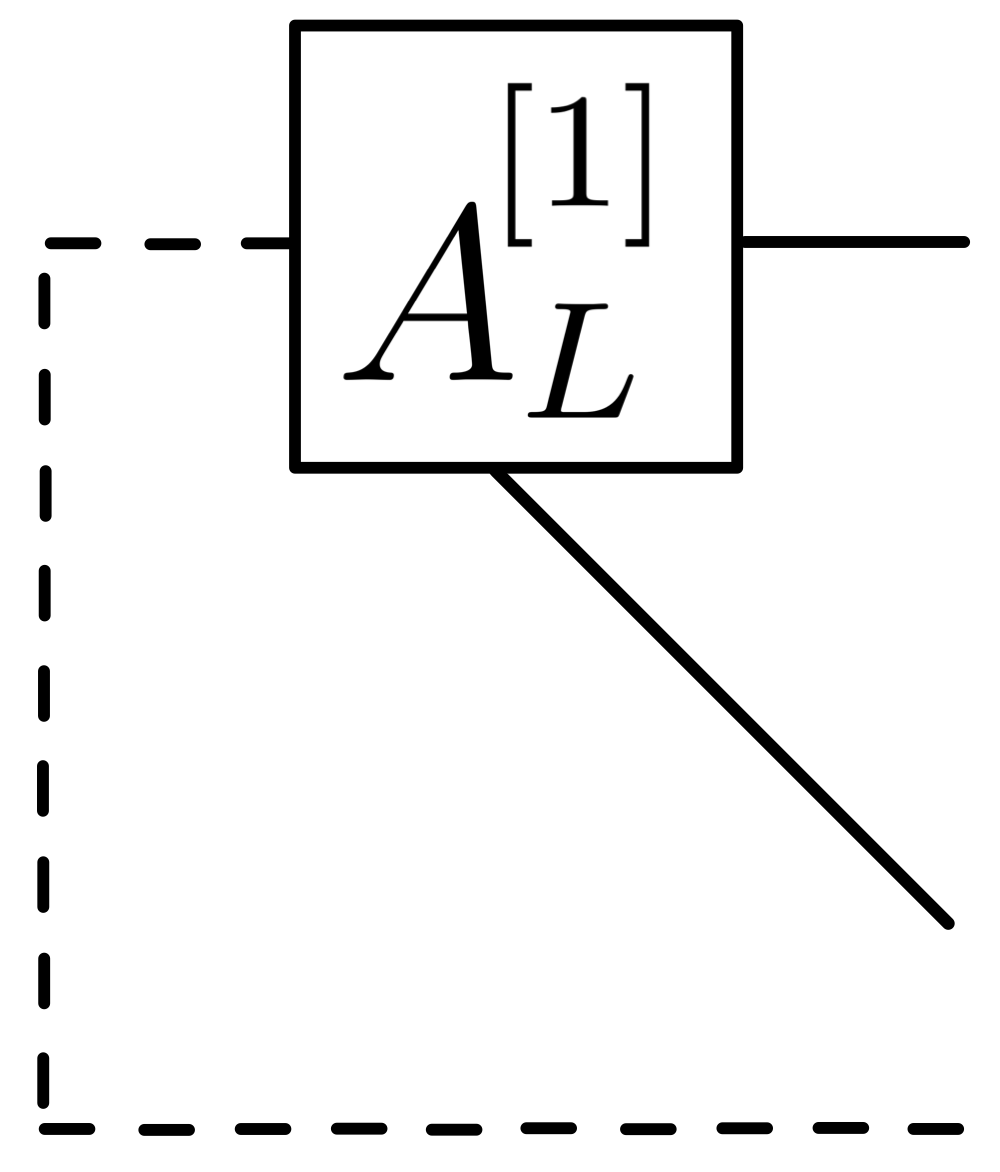
\includegraphics[height=1.6cm]{TdaggerL2.png}} 
\hspace{1em}& ; &
	\raisebox{-0.5\height}{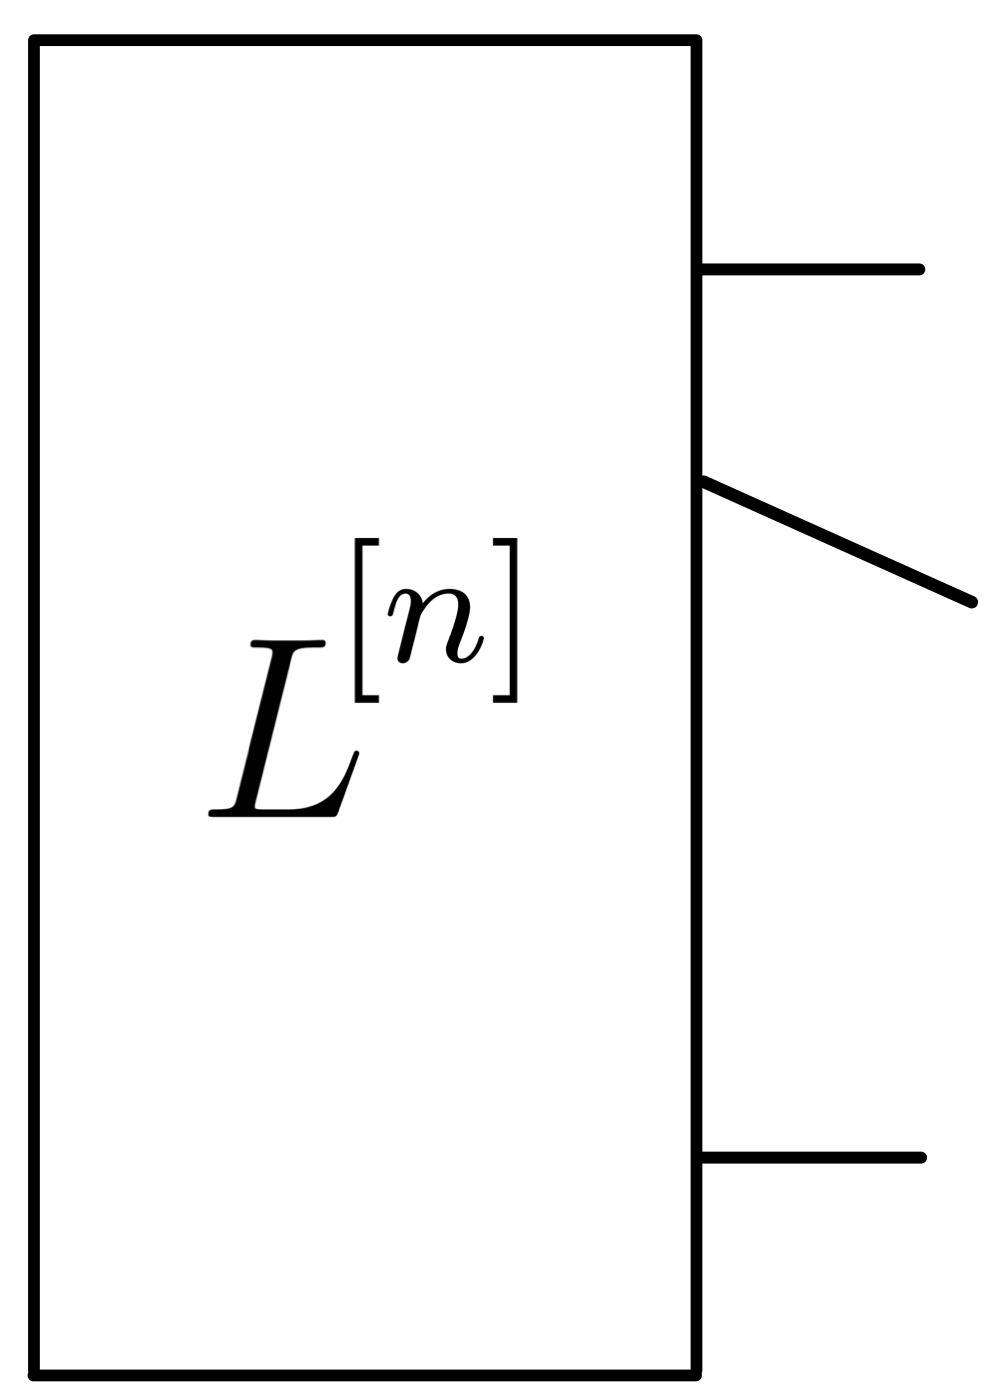
\includegraphics[height=2.cm]{TdaggerL3.png}} 
	\:=\:
	\raisebox{-0.5\height}{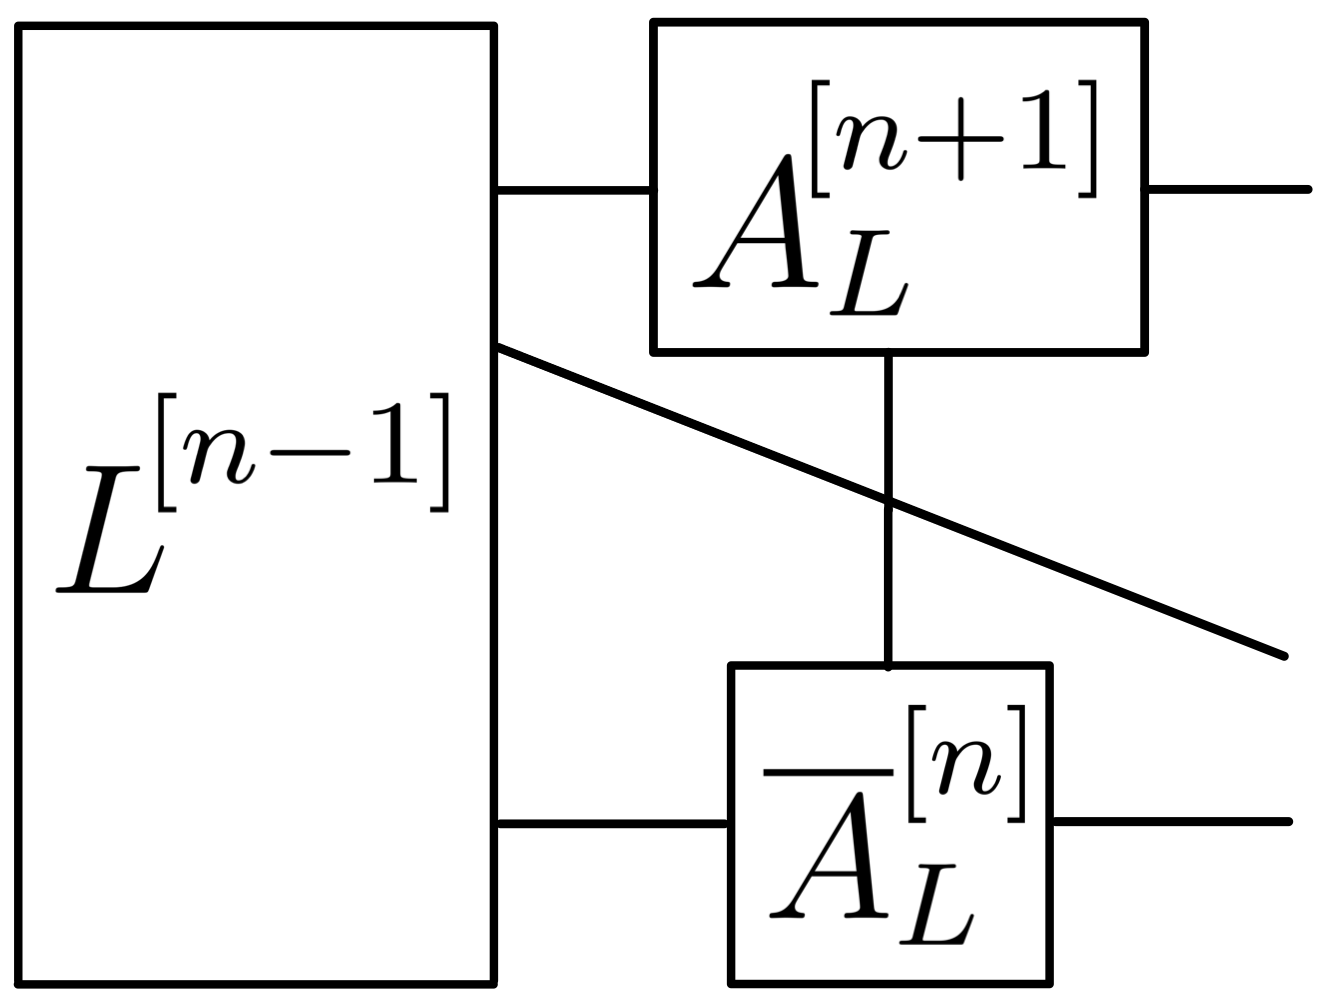
\includegraphics[height=2.cm]{TdaggerL4.png}}
	\hspace{1em} \text{\scriptsize{$(n = 1, \ldots, N-1)$}}
\\[3em]
	\raisebox{-0.5\height}{\includegraphics[height=2.cm]{TdaggerLB1.png}} 
	\:=\: 
	\raisebox{-0.5\height}{\includegraphics[height=1.6cm]{TdaggerLB2.png}} 
& ; &
	\raisebox{-0.5\height}{\includegraphics[height=2.cm]{TdaggerLB3.png}} 
	\:=\: 
	\raisebox{-0.5\height}{\includegraphics[height=2.cm]{TdaggerLB4.png}}
	\:+\:
	\raisebox{-0.5\height}{\includegraphics[height=2.cm]{TdaggerLB5.png}}
	\hspace{1em} \text{\scriptsize{$(n = 1, \ldots, N-1)$}}
\\[3em]
	\raisebox{-0.5\height}{\includegraphics[height=2.cm]{TdaggerR1.png}} 
	\:=\:
	\raisebox{-0.5\height}{\includegraphics[height=1.6cm]{TdaggerR2.png}} 
& ; &
	\raisebox{-0.5\height}{\includegraphics[height=2.cm]{TdaggerR3.png}} 
	\:=\: 
	\raisebox{-0.5\height}{\includegraphics[height=2.cm]{TdaggerR4.png}}
	\hspace{1em} \text{\scriptsize{$(n = N-1, \ldots, 2)$}}
\\[3em]
	\raisebox{-0.5\height}{\includegraphics[height=2.cm]{TdaggerRB1.png}} 
	\:=\: 0
& ; &
	\raisebox{-0.5\height}{\includegraphics[height=2.cm]{TdaggerRB2.png}} 
	\:=\: 
	\raisebox{-0.5\height}{\includegraphics[height=2.cm]{TdaggerRB3.png}}
	\:+\:
	\raisebox{-0.5\height}{\includegraphics[height=2.cm]{TdaggerRB4.png}}
	\hspace{1em} \text{\scriptsize{$(n = N-1, \ldots, 2)$}}
\end{array}
\end{equation*}


% EFFECTIVE HAMILTONIAN FOR ISOPEPS VQPE
\newpage
\section*{Effective Hamiltonian for isoPEPS quasiparticle excitations}
We show all terms that appear when sandwiching the Hamiltonian \eqref{eq:column_mpo} between the ket superposition \eqref{eq:ket_B} and a single bra state of the latter. Since we are ultimately interested in implementing the effective Hamiltonian $\left[ H_{\text{eff}} \vert B ) \right]^{[n_x, y]} = \partial_{\overline{B}^{[n_x, y]}} \langle \psi(\overline{B}^{[n_x]}) \vert H \vert \psi(B) \rangle$ with compressed bMPS, we move the ket excitations and column MPO Hamiltonians relative to the bra column $\overline{B}^{[n_x]}$ (here exemplarily for $n_x = 4$):
\begin{center}
\vspace*{-0.5em}
\includegraphics[height=20cm]{B4_H_B.pdf}
\end{center}

